\documentclass[journal,a4paper,onecolumn]{IEEEtran}

% ===== Encoding & language (Slovak) =====
\usepackage[T1]{fontenc}
\usepackage[utf8]{inputenc}
\usepackage[slovak]{babel}

% *** GRAPHICS RELATED PACKAGES ***
\ifCLASSINFOpdf
   \usepackage[pdftex]{graphicx}
   \graphicspath{{./pdf/}{./jpeg/}{./eps/}{./plots/}}
   \DeclareGraphicsExtensions{.pdf,.jpeg,.png}
\else
   \usepackage[dvips]{graphicx}
   \graphicspath{{./eps/}}
   \DeclareGraphicsExtensions{.eps}
\fi

% ===== Math, lists, tables =====
\usepackage{amsmath}
\usepackage{amssymb}   % \mathbb, \checkmark, \lll
\usepackage{textcomp}  % \texttimes
\usepackage{booktabs}
\let\labelindent\relax
\usepackage{enumitem}

% Slovak quotation marks (\uv) — defined manually because babel 'slovak' option
% is unavailable in this TeX distribution; \quotedblbase / \textquotedblleft
% are provided by T1 fontenc (already loaded).
\newcommand{\uv}[1]{\quotedblbase#1\textquotedblleft}

% ===== Links =====
\usepackage{hyperref}
\hypersetup{colorlinks, linkcolor=black, urlcolor=blue, citecolor=black, filecolor=black, menucolor=black}
\usepackage{url}
\usepackage{lastpage}
\usepackage{array}

% \lll redefined as binary operator (rotation in ChaCha20 formulas)
\let\lllRel\lll
\renewcommand{\lll}{\mathbin{\lllRel}}

% correct bad hyphenation here
\hyphenation{op-tical net-works semi-conduc-tor}

\begin{document}
\addtocounter{page}{1}

\title{~\vskip -5mm Zvýšenie bezpečnosti vybraných šifrovacích algoritmov v prístupových systémoch}

\author{\textit{\begin{Large}\textsuperscript{1}Oleksandr~MYKHAILYSHYN\end{Large}}\\
\bigskip
\textsuperscript{1}Katedra počítačov a informatiky, Fakulta elektrotechniky a informatiky, Technická univerzita v Ko\v{s}iciach, Slovenská republika\\
\bigskip
\textsuperscript{1}oleksandr.mykhailyshyn@student.tuke.sk}

\maketitle

\begin{abstract}
\textbf{\textit{Abstrakt}}~\textendash~\bfseries
Práca sa zaoberá bezpečnostnými mechanizmami, ktoré sú relevantné pre moderné systémy kontroly prístupu využívajúce bezkontaktné identifikátory RFID/NFC. Teoretická časť nevystupuje iba ako všeobecný prehľad, ale priamo nadväzuje na vytvorený prototyp: čítačku založenú na ESP32 a RC522, serverovú aplikáciu v jazyku C++ a lokálne úložisko SQLite s auditnou stopou. Jadrom návrhu je otázka, ako zvýšiť dôveryhodnosť celého toku udalosti od načítania UID až po rozhodnutie o prístupe a neskoršie overenie auditu.

V texte preto rozoberám autentifikáciu hardvérových požiadaviek pomocou HMAC-SHA-256, ochranu proti opakovaniu správ cez monotónne \texttt{hw\_seq}, vnútorný frame chránený mechanizmom AEAD (ChaCha20-Poly1305 a XChaCha20-Poly1305) a auditný log navrhnutý tak, aby bolo možné odhaliť dodatočnú manipuláciu. V experimentálnej časti sa porovnáva šesť konfiguračných profilov, ktoré kombinujú oba šifrovacie algoritmy s tromi stratégiami generovania nonce (náhodný, deterministický HMAC a deterministický s runtime anomálnou detekciou). Súčasne otvorene pomenúvam aj hranice prototypu: UID karty je v tomto riešení identifikátor, nie kryptografický dôkaz identity, databáza je uložená lokálne a prototyp nevyžaduje povinné TLS. Tieto obmedzenia nie sú obchádzané, ale slúžia ako súčasť realistického hodnotenia toho, čo prototyp chráni dobre a kde zostáva priestor na ďalšie rozšírenie.
\end{abstract}

\begin{IEEEkeywords}
\textbf{\textit{Kľúčové slová}}~\textendash~\bfseries
kontrola prístupu, RFID, NFC, kryptografia, AEAD, ChaCha20-Poly1305, XChaCha20-Poly1305, anomálna detekcia, HMAC, HKDF, anti-replay, audit log.
\end{IEEEkeywords}

% =============================================================
%  ABSTRAKT V ANGLICKOM JAZYKU
% =============================================================
\clearpage
\begin{center}
  {\large\textbf{Enhancing Security of Selected Encryption Algorithms\\[0.2em]in Access Control Systems}}\\[0.8em]
  \textit{\textbf{Oleksandr Mykhailyshyn}}\\[0.3em]
  Technical University of Ko\v{s}ice, Faculty of Electrical Engineering and Informatics, Slovakia
\end{center}

\bigskip
\noindent\textbf{Abstract}~\textendash~
The thesis addresses security mechanisms relevant to modern RFID/NFC access control systems.
The theoretical part does not serve merely as a general overview but directly underpins the
implemented prototype: an ESP32 and RC522-based reader, a C++ server application, and a local
SQLite storage with an audit trail. The core design question is how to increase the
trustworthiness of the entire event flow from UID reading to the access decision and subsequent
audit verification.

\medskip
\noindent
The text therefore examines the authentication of hardware requests using HMAC-SHA-256,
protection against message replay via monotonic \texttt{hw\_seq}, an internal frame protected by
AEAD (ChaCha20-Poly1305 and XChaCha20-Poly1305), and an audit log designed to detect post-hoc
manipulation. The experimental section compares six configuration profiles that combine both
encryption algorithms with three nonce generation strategies (random, deterministic HMAC, and
deterministic with runtime anomaly detection). The thesis also explicitly identifies the
prototype's limitations: the card UID is an identifier in this solution, not a cryptographic
proof of identity; the database is stored locally; and TLS is not mandatory. These constraints
are not circumvented but serve as part of a realistic assessment of what the prototype protects
well and where room for further improvement remains.

\bigskip
\noindent\textbf{Keywords}~\textendash~
access control, RFID, NFC, cryptography, AEAD, ChaCha20-Poly1305, XChaCha20-Poly1305,
anomaly detection, HMAC, HKDF, anti-replay, audit log.

% =============================================================
%  ČESTNÉ VYHLÁSENIE
% =============================================================
\clearpage
\vspace*{4cm}
\begin{center}
  {\Large\textbf{ČESTNÉ VYHLÁSENIE}}
\end{center}

\vspace{2.5cm}
\noindent
Vyhlasujem, že som celú diplomovú prácu vypracoval samostatne a uviedol som všetku použitú
literatúru.

\vspace{4cm}
\noindent
\begin{tabular}{@{}p{7cm} p{7cm}@{}}
 & \dotfill \\
 & \centering Oleksandr Mykhailyshyn
\end{tabular}

\vspace{1cm}
\noindent
Košice, \today

% =============================================================
%  POĎAKOVANIE
% =============================================================
\clearpage
\vspace*{4cm}
\begin{center}
  {\Large\textbf{POĎAKOVANIE}}
\end{center}

\vspace{2cm}
\noindent
Ďakujem vedúcemu diplomovej práce za odborné vedenie, cenné rady a trpezlivú podporu počas
celého procesu vypracovania tejto práce.

% =============================================================
%  OBSAH (TABLE OF CONTENTS)
% =============================================================
\clearpage
\tableofcontents

% =============================================================
%  ZOZNAM OBRÁZKOV (LIST OF FIGURES)
% =============================================================
\clearpage
\listoffigures

% =============================================================
%  ZOZNAM SKRATIEK
% =============================================================
\clearpage
\begin{center}
  {\Large\textbf{ZOZNAM SKRATIEK}}
\end{center}

\bigskip\noindent
\begin{tabular}{>{\bfseries}p{2.8cm} p{12.2cm}}
AEAD   & Authenticated Encryption with Associated Data \\[2pt]
ABAC   & Attribute-Based Access Control \\[2pt]
AAA    & Authentication, Authorization, Accounting \\[2pt]
ARX    & Add-Rotate-XOR \\[2pt]
CIA    & Confidentiality, Integrity, Availability \\[2pt]
DAC    & Discretionary Access Control \\[2pt]
DoS    & Denial of Service \\[2pt]
ESP32  & mikrokontrolér Espressif Systems ESP32 \\[2pt]
FEI    & Fakulta elektrotechniky a informatiky \\[2pt]
FIPS   & Federal Information Processing Standard \\[2pt]
GDPR   & General Data Protection Regulation \\[2pt]
HKDF   & HMAC-based Key Derivation Function \\[2pt]
HMAC   & Hash-based Message Authentication Code \\[2pt]
HSM    & Hardware Security Module \\[2pt]
IoT    & Internet of Things \\[2pt]
KPI    & Katedra počítačov a informatiky \\[2pt]
LSan   & LeakSanitizer \\[2pt]
MAC    & Message Authentication Code \\[2pt]
MITM   & Man-in-the-Middle (útok) \\[2pt]
mTLS   & mutual Transport Layer Security \\[2pt]
NFC    & Near Field Communication \\[2pt]
NIST   & National Institute of Standards and Technology \\[2pt]
NVS    & Non-Volatile Storage \\[2pt]
OSDP   & Open Supervised Device Protocol \\[2pt]
OTA    & Over-The-Air (bezdrôtová aktualizácia) \\[2pt]
OWASP  & Open Web Application Security Project \\[2pt]
PKI    & Public Key Infrastructure \\[2pt]
PSK    & Pre-Shared Key \\[2pt]
RBAC   & Role-Based Access Control \\[2pt]
RC522  & čítačka RFID kariet (NXP Semiconductors) \\[2pt]
RFC    & Request for Comments \\[2pt]
RFID   & Radio Frequency Identification \\[2pt]
SIMD   & Single Instruction, Multiple Data \\[2pt]
SQLite & odľahčená relačná databáza (serverless) \\[2pt]
STRIDE & Spoofing, Tampering, Repudiation, Information Disclosure, Denial of Service, Elevation of Privilege \\[2pt]
TLS    & Transport Layer Security \\[2pt]
TUKE   & Technická univerzita v Košiciach \\[2pt]
UBSan  & UndefinedBehaviorSanitizer \\[2pt]
UID    & Unique Identifier \\[2pt]
\end{tabular}

\clearpage

\section{Úvod}

Systémy kontroly prístupu (\emph{Access Control Systems}) sú jedným z tých prvkov infraštruktúry, pri ktorých sa fyzická a informačná bezpečnosť stretávajú priamo v jednom bode. Na prvý pohľad ide iba o rozhodnutie, či sa dvere otvoria alebo nie. V skutočnosti sa za tým skrýva identifikácia používateľa, vyhodnotenie pravidiel, práca s tajomstvami, komunikácia po sieti a napokon aj audit, ktorý má po incidente vysvetliť, čo sa stalo.

Práve pri jednoduchších riešeniach býva rozdiel medzi funkčným a bezpečným systémom najvýraznejší. V praxi nie je problém zostaviť čítačku, ktorá po načítaní UID pošle hodnotu na server a čaká na odpoveď. Takýto návrh je však zraniteľný takmer okamžite: stačí zachytiť požiadavku, zopakovať ju v inom čase, podvrhnúť vlastný identifikátor alebo upraviť dáta v úložisku. Ak systém ukladá surové UID a pritom nemá dôveryhodný audit, po incidente zostáva iba veľmi slabá stopa.

Táto diplomová práca vychádza práve z takéhoto praktického pozorovania. Cieľom nebolo navrhnúť teoreticky maximálne silný systém bez ohľadu na cenu a zložitosť, ale postaviť prototyp, na ktorom sa dá ukázať, ktoré bezpečnostné mechanizmy majú v prístupových systémoch skutočný prínos. Výsledkom je kombinácia hardvéru (ESP32 + RC522), serverovej aplikácie v jazyku C++ a webového rozhrania, v ktorom sa spravujú čítačky, dvere, roly, karty aj auditné záznamy.

Bezpečnosť riešenia stojí na niekoľkých navzájom previazaných vrstvách:

\begin{itemize}[leftmargin=*,itemsep=2pt]
  \item autentifikácia hardvérových požiadaviek pomocou HMAC-SHA-256\cite{FIPS1981},
  \item šifrovanie a integrita interného payloadu pomocou AEAD (ChaCha20-Poly1305\cite{RFC8439} a XChaCha20-Poly1305\cite{XChaChaDraft,LibsodiumXChaChaDoc}),
  \item ochrana proti replay útokom cez monotónne sekvencie a \emph{ReplayWindow},
  \item ochrana súkromia identifikátorov kariet pomocou HMAC hashovania s \emph{pepper},
  \item auditná stopa navrhnutá tak, aby bolo možné odhaliť dodatočnú manipuláciu pomocou HMAC hash chain a anchor bodov\cite{SchneierKelsey1999}.
\end{itemize}

Zjednodušená schéma celého toku udalosti je znázornená na obrázku~\ref{fig:e2e_overview}.

Dôležité je, že jednotlivé vrstvy v prototype neplnia tú istú úlohu. Hardvérová čítačka neposiela na server priamo AEAD šifrovaný payload; odosiela HTTP požiadavku autentifikovanú pomocou HMAC a monotónneho \texttt{hw\_seq}. Až server po overení tejto požiadavky vytvára interný kryptograficky chránený frame, ktorý vstupuje do rozhodovacej logiky. Táto hranica dôvery je v texte pomenovaná zámerne, pretože ovplyvňuje aj interpretáciu výsledkov: niečo iné znamená ochrana proti podvrhnutiu HTTP požiadavky a niečo iné ochrana interného frame alebo auditnej stopy.

Bezpečnostná analýza pokrýva oblasti s priamym dopadom na implementovaný systém: model hrozieb, kryptografické primitíva, autentifikáciu zariadenia, anti-replay mechanizmy, správu kľúčov a auditovateľnosť. Overenie prínosu navrhnutých mechanizmov vychádza z experimentálneho porovnania šiestich konfiguračných profilov, ktoré variujú šifrovací algoritmus, stratégiu generovania nonce a prítomnosť runtime anomálnej detekcie.


\begin{figure}[!ht]
\centering
\fbox{\parbox{0.93\linewidth}{\centering
\textbf{Karta / UID} $\rightarrow$ \textbf{ESP32 + RC522} $\rightarrow$ \textbf{HTTP požiadavka}\\[2mm]
\textbf{HMAC + \texttt{hw\_seq}} $\rightarrow$ \textbf{C++ server} $\rightarrow$ \textbf{interný frame (AEAD)}\\[2mm]
\textbf{DecisionEngine} $\rightarrow$ \textbf{SQLite + audit chain} $\rightarrow$ \textbf{Web UI / live logs}
}}
\caption{Zjednodušená end-to-end schéma prototypu a hraníc dôvery medzi vrstvami.}
\label{fig:e2e_overview}
\end{figure}

% ==============================================================
\section{Motivácia, ciele a prínos práce}

\subsection{Motivácia}

Motivácia tejto práce nie je iba teoretická. Počas návrhu a skladania prototypu sa opakovane ukazovalo, že najjednoduchšia funkčná verzia systému by sa dala postaviť veľmi rýchlo: prečítať UID, poslať ho na server a podľa odpovede otvoriť dvere. Takýto návrh však rieši iba funkcionalitu, nie dôveryhodnosť. Hneď ako sa do úvahy vezme bežná lokálna sieť, databáza s kartami a potreba spätne vysvetliť incident, začnú byť zaujímavé celkom iné otázky.

Reálne prostredie totiž zahŕňa:

\begin{itemize}[leftmargin=*,itemsep=2pt]
  \item nepredvídateľnú sieť (Wi-Fi, zdieľané siete, kompromitované zariadenia),
  \item úložisko v podobe databázy, ktorú je možné kopírovať a analyzovať,
  \item insider scenáre (administrátor, ktorý môže zneužiť oprávnenia alebo zmeniť logy),
  \item vstavané zariadenia s obmedzenými zdrojmi, ktoré často nemajú plnú podporu pre komplexné bezpečnostné protokoly.
\end{itemize}

Ak systém nepoužíva kryptograficky zabezpečené logovanie, útočník môže po incidente vymazať stopy. Ak systém neobsahuje anti-replay, je možné prístup opakovať bez karty. Ak systém ukladá surové UID, únik databázy priamo ohrozuje používateľov.

\subsection{Ciele práce}

Hlavné ciele práce sú:

\begin{enumerate}[leftmargin=*,itemsep=2pt]
  \item Navrhnúť bezpečnostné požiadavky a model hrozieb pre prototyp prístupového systému.
  \item Zaviesť kryptografické mechanizmy na úrovni komunikácie a spracovania:
  \begin{itemize}[leftmargin=*,itemsep=2pt]
    \item AEAD (ChaCha20-Poly1305 a XChaCha20-Poly1305) pre dôvernosť a integritu dát\cite{RFC8439,XChaChaDraft},
    \item HMAC-SHA-256 pre autentifikáciu požiadaviek hardvéru\cite{FIPS1981},
    \item HKDF pre deriváciu kľúčov a oddelenie účelov\cite{RFC5869}.
  \end{itemize}
  \item Implementovať anti-replay mechanizmus založený na monotónnom \texttt{hw\_seq} (perzistentne uloženom na ESP32) a \emph{ReplayWindow} na serveri.
  \item Navrhnúť a implementovať tamper-evident audit log s možnosťou verifikácie a detekcie truncation.
  \item Stanoviť analytické ciele hodnotenia: porovnať šesť konfiguračných profilov (dva AEAD algoritmy $\times$ tri nonce stratégie) v šiestich útokových a výkonnostných scenároch, zbierať metriky (úspešnosť útoku, dôvody zamietnutia, latenciu a priepustnosť) a formulovať závery o príspevku jednotlivých bezpečnostných mechanizmov.
\end{enumerate}

\subsection{Prínos}

Prínos práce je možné čítať v dvoch rovinách. Prvá je technická: vznikol funkčný prototyp, na ktorom sa dá ukázať, že aj pomerne malý prístupový systém môže mať jasne oddelené bezpečnostné vrstvy. Druhá rovina je metodická: práca nevychádza len z tvrdenia, že zvolený mechanizmus je „bezpečnejší“, ale pripravuje priestor na jeho meranie a porovnanie s jednoduchšou verziou riešenia.

Konkrétne ide o:

\begin{itemize}[leftmargin=*,itemsep=2pt]
  \item demonštrácia realistického návrhu bezpečnej komunikácie pre IoT/embedded zariadenia,
  \item dôsledné oddelenie autentifikácie hardvéru od administrátorských oprávnení (HW nepoužíva admin token),
  \item ochrana súkromia používateľov pomocou hashovania identifikátorov kariet,
  \item auditovateľnosť a detekcia manipulácie logov pomocou kryptografických reťazcov,
  \item modulárna architektúra C++ projektu (kryptografia, protokol, rozhodovanie, úložisko, UI).
\end{itemize}

\subsection{Rozsah riešenia a vedomé obmedzenia}

V tejto práci nepovažujem za poctivé tváriť sa, že prototyp rieši všetky problémy produkčného prístupového systému. Niektoré voľby boli urobené zámerne, pretože cieľom bolo overiť konkrétne bezpečnostné mechanizmy a nie simulovať kompletné enterprise nasadenie.

Použitá RFID karta pracuje v jednoduchom režime, takže UID vystupuje ako identifikátor, nie ako kryptografický dôkaz identity. Databázová vrstva je postavená na SQLite, čo je pre prototyp a experimenty praktické, ale neznamená to vysokú dostupnosť, centralizovanú správu tajomstiev ani pohodlné škálovanie. Komunikácia hardvéru so serverom je v základnom režime chránená autentifikáciou a integritou na aplikačnej vrstve (HMAC + \texttt{hw\_seq}), zatiaľ čo dôvernosť transportu cez TLS zostáva rozšírením pre ďalšie nasadenie.

Tieto obmedzenia teda nie sú slabinou textu, ktorú by bolo potrebné zakryť. Naopak, vytvárajú presný rámec pre interpretáciu výsledkov. Ak sa v analytickej časti ukáže zlepšenie odolnosti voči podvrhnutiu, replay alebo manipulácii s auditom, bude zrejmé, že ide o prínos navrhnutých mechanizmov v rámci definovaného prototypu, nie o všeobecné tvrdenie o všetkých prístupových systémoch.


\begin{table}[!ht]
\renewcommand{\arraystretch}{1.3}
\centering
\caption{Vedomé obmedzenia prototypu a ich význam pre interpretáciu výsledkov}
\label{tab:prototype_limits}
\small
\begin{tabular}{p{0.24\linewidth} p{0.30\linewidth} p{0.36\linewidth}}
\toprule
\textbf{Oblasť} & \textbf{Aktuálne riešenie} & \textbf{Dôsledok pre prácu} \\
\midrule
Identita karty & UID slúži ako identifikátor, nie ako kryptografický dôkaz & Práca sa zameriava najmä na bezpečnosť komunikácie, serverovej logiky a auditu, nie na bezpečné smart karty. \\
Úložisko & Lokálna SQLite databáza & Riešenie je vhodné pre prototyp a experimenty; vysoká dostupnosť a centralizovaná správa tajomstiev nie sú predmetom práce. \\
Transport & Povinné TLS nie je v základnom režime nasadené & Dôvernosť prenosu UID nie je hlavnou demonštrovanou vlastnosťou; dôraz je na autentifikáciu zariadenia, anti-replay a auditovateľnosť. \\
Správa tajomstiev & Tajomstvá sú spravované pragmaticky pre potreby prototypu & Výsledky treba interpretovať ako experimentálny návrh, nie ako plnohodnotné produkčné nasadenie. \\
\bottomrule
\end{tabular}
\normalsize
\end{table}

\subsection{Metodika hodnotenia a analytické ciele}

Pri podobných prototypoch sa často končí pri ukážke, že systém „funguje“. To však pre tému zameranú na bezpečnosť nestačí. Preto je hodnotenie od začiatku postavené tak, aby bolo možné overiť, či navrhnuté mechanizmy skutočne menia správanie systému pri útoku alebo chybe.

V praktickej časti sa preto nebude sledovať iba to, či server vráti \texttt{allow} alebo \texttt{deny}. Dôležité bude aj to, prečo k rozhodnutiu došlo, aká je úspešnosť jednotlivých útokov, akú latenciu zavádzajú ochranné mechanizmy a ako sa riešenie správa pri opakovaných alebo chybných požiadavkách. Porovnanie základného a zabezpečeného variantu je zvolené práve preto, aby analytická časť prirodzene vyrástla z cieľov definovaných v teórii a nepôsobila ako neskôr doplnený experimentálny dodatok.


\begin{table}[!ht]
\renewcommand{\arraystretch}{1.3}
\centering
\caption{Prepojenie analytických cieľov s meranými ukazovateľmi}
\label{tab:analytics_goals}
\small
\begin{tabular}{p{0.27\linewidth} p{0.29\linewidth} p{0.30\linewidth}}
\toprule
\textbf{Scenár} & \textbf{Mechanizmus} & \textbf{Pozorovaný ukazovateľ} \\
\midrule
Podvrhnutie HW požiadavky & HMAC-SHA-256 & Miera zamietnutia, dôvod \texttt{bad\_signature}. \\
Replay zachytenej požiadavky & \texttt{hw\_seq} + ReplayWindow & Miera zamietnutia, dôvod \texttt{replay} alebo \texttt{too\_old}. \\
Manipulácia interného frame & AEAD + AAD & Neúspešné overenie integrity a zamietnutie správy. \\
Zásah do auditnej stopy & HMAC hash chain + anchor & Úspešnosť detekcie pri verifikácii auditu. \\
Prevádzková záťaž & Validácia vstupu + rozhodovanie & Latencia spracovania a správanie systému pri opakovaných požiadavkách. \\
\bottomrule
\end{tabular}
\normalsize
\end{table}

% ==============================================================
\section{Všeobecné bezpečnostné pojmy a terminológia}

Táto kapitola predstavuje základné pojmy, ktoré sa používajú v ďalších častiach práce.

\subsection{CIA triáda a rozšírené bezpečnostné ciele}

CIA triáda (dôvernosť, integrita, dostupnosť) je základný rámec, od ktorého sa pri bezpečnostnom návrhu zvyčajne začína. V prístupovom systéme však sama osebe nestačí. Pri praktickej implementácii sa veľmi rýchlo ukáže, že rovnako podstatné je vedieť, kto správu vytvoril, či ju nemožno znovu použiť a či sa dá po incidente spätne overiť história udalostí. Preto je vhodné k CIA doplniť ešte niekoľko cieľov:

\begin{itemize}[leftmargin=*,itemsep=2pt]
  \item autentickosť (\emph{authenticity}) -- schopnosť overiť pôvod správy alebo akcie,
  \item auditovateľnosť (\emph{auditability}) -- schopnosť spätne preukázať rozhodnutia a udalosti,
  \item odolnosť voči replay (\emph{replay resistance}) -- schopnosť odmietnuť opakovanie starej správy.
\end{itemize}

V prototype sa tieto ciele prejavujú veľmi konkrétne:

\begin{itemize}[leftmargin=*,itemsep=2pt]
  \item Dôvernosť: útočník nemá získať citlivé údaje (napr. identifikátory, tokeny, kľúče).
  \item Integrita: útočník nemá zmeniť požiadavku alebo audit záznam bez detekcie.
  \item Dostupnosť: systém musí zvládnuť prevádzku bez výpadkov; zároveň sa musí brániť proti DoS v rámci možností prototypu.
\end{itemize}


\begin{table}[!ht]
\renewcommand{\arraystretch}{1.3}
\centering
\caption{Mapovanie bezpečnostných cieľov na mechanizmy použité v prototype}
\label{tab:security_mapping}
\small
\begin{tabular}{p{0.22\linewidth} p{0.33\linewidth} p{0.29\linewidth}}
\toprule
\textbf{Cieľ} & \textbf{Mechanizmus v prototype} & \textbf{Príklad narušenia} \\
\midrule
Dôvernosť & AEAD frame, neukladanie surového UID & Čítanie citlivých údajov z payloadu alebo databázy. \\
Integrita & HMAC požiadavky, AEAD tag, hash chain auditu & Zmena \texttt{uid}, \texttt{door\_id} alebo auditnej udalosti bez detekcie. \\
Dostupnosť & Limity vstupu, fail-closed, validácia & Pád parsera alebo vyčerpanie zdrojov pri chybných vstupoch. \\
Autentickosť & HMAC-SHA-256 pre hardvér & Vydávanie sa za legitímnu čítačku. \\
Odolnosť voči replay & \texttt{hw\_seq} + ReplayWindow & Opakované použitie starej platnej požiadavky. \\
Auditovateľnosť & Tamper-evident audit log + verify nástroj & Dodatočné popretie udalosti alebo tichá úprava histórie. \\
\bottomrule
\end{tabular}
\normalsize
\end{table}

\subsection{AAA model: Authentication, Authorization, Accounting}

Model AAA je v literatúre známy a pomerne stručný, no v kontexte tejto práce je užitočný práve preto, že sa dá priamo premietnuť do implementácie. Namiesto abstraktného delenia sa dá pri prototype ukázať, kde sa ktorá časť naozaj nachádza:

\begin{itemize}[leftmargin=*,itemsep=2pt]
  \item Authentication (autentifikácia) -- overenie identity alebo pôvodu.
  \item Authorization (autorizácia) -- rozhodnutie, či identita môže vykonať akciu.
  \item Accounting (účtovanie/audit) -- záznam akcií a ich výsledkov.
\end{itemize}

V tomto prototype je autentifikácia rozdelená na dve vrstvy. Karta slúži predovšetkým ako identifikátor používateľa, zatiaľ čo samotné zariadenie sa voči serveru preukazuje podpisom HMAC. Autorizácia prebieha v \emph{DecisionEngine} na základe rolí a väzieb medzi čítačkou a dverami. Posledná časť modelu, teda accounting, nie je iba pomocný log pre administrátora; je to auditná stopa, z ktorej má byť možné spätne overiť, čo sa stalo a či s históriou nebolo manipulované. V tomto bode sa teoretický model AAA prirodzene prepája s odporúčaniami pre digitálnu identitu a správu logov.\cite{NIST80063B4,NIST80092}

\subsection{Riziko, hrozba, zraniteľnosť}

V ďalších kapitolách sa opakovane pracuje s pojmami hrozba, zraniteľnosť a riziko, preto má zmysel ich hneď na začiatku oddeliť. Bez tohto rozlíšenia by bolo ťažké vysvetliť, prečo sa niektoré mechanizmy zavádzajú priamo do protokolu a iné iba ako odporúčanie pre budúce nasadenie.

Bezpečnostná analýza preto rozlišuje:

\begin{itemize}[leftmargin=*,itemsep=2pt]
  \item hrozbu (threat) -- potenciálnu príčinu incidentu (napr. útočník schopný zachytiť sieťovú komunikáciu),
  \item zraniteľnosť (vulnerability) -- slabinu systému (napr. absencia anti-replay),
  \item riziko (risk) -- kombináciu pravdepodobnosti a dopadu.
\end{itemize}

V tejto práci nie je cieľom vytvoriť úplný korporátny register rizík. Dôležitejšie je ukázať, ktoré hrozby sú pre zvolený prototyp realistické a ktoré mechanizmy ich vedia znížiť na prijateľnú mieru.

\subsection{Modelovanie hrozieb}

Pri návrhu prototypu sa ukázalo, že hrozby sa dajú najlepšie udržať pod kontrolou vtedy, keď sú pomenované ešte pred implementáciou. Ako orientačný rámec je preto vhodný model STRIDE\cite{STRIDE} (Spoofing, Tampering, Repudiation, Information disclosure, Denial of service, Elevation of privilege). Nie všetky jeho časti sú v tejto práci rovnako dôležité; najviac sa týkajú tých vrstiev, ktoré prototyp naozaj obsahuje:

\begin{itemize}[leftmargin=*,itemsep=2pt]
  \item Spoofing: podvrhnutie požiadavky (riešené HMAC),
  \item Tampering: zmena dát alebo logov (riešené AEAD, audit hash chain),
  \item Repudiation: popieranie udalostí (riešené auditom),
  \item Information disclosure: únik identifikátorov (riešené hashovaním UID v DB a odporúčaním TLS),
  \item DoS: zahltenie endpointu (čiastočne riešené limitmi a validáciou).
\end{itemize}



\subsection{Autentifikačné faktory a pojem identity}

V prístupových systémoch sa často hovorí o tom, že používateľ sa \uv{identifikuje kartou}. Je dôležité rozlišovať dva pojmy: identifikácia (tvrdenie \uv{kto som}) a autentifikácia (dôkaz, že tvrdenie je pravdivé). V praxi sa autentifikácia realizuje pomocou \emph{faktorov}:

\begin{itemize}[leftmargin=*,itemsep=2pt]
  \item niečo, čo mám (karta, token, zariadenie),
  \item niečo, čo viem (PIN, heslo),
  \item niečo, čím som (biometria).
\end{itemize}

RFID/NFC karta v jednoduchom režime (iba UID) je teda skôr identifikátor než plnohodnotný autentifikátor. V produkčných systémoch sa tento problém zvykne riešiť ďalším faktorom, napríklad PIN-om, alebo kartou s vlastným kryptografickým protokolom. V tejto práci sa tento rozdiel neskrýva; naopak, je súčasťou interpretácie výsledkov. Riziko sa kompenzuje inde -- najmä autentifikáciou zariadenia voči serveru, anti-replay mechanizmami a auditovateľnosťou. Z pohľadu odporúčaní pre digitálnu identitu ide teda o prototyp s jednoduchším poverením používateľa, ale so silnejšou ochranou komunikačnej a serverovej vrstvy.\cite{NIST80063B4,FIPS2013}

\subsection{Zodpovednosť, nepopierateľnosť a forenzná pripravenosť}

V praxi nestačí iba rozhodnúť \emph{ALLOW/DENY}. Organizácia potrebuje vedieť \emph{kedy}, \emph{kde} a \emph{prečo} k rozhodnutiu došlo. Tento aspekt sa často označuje ako accountability (zodpovednosť) a je úzko spojený s auditovateľnosťou.

Pojem \emph{nepopierateľnosť} (non-repudiation) sa v kryptografii spája najmä s digitálnymi podpismi, ale v kontexte prístupových systémov má aj praktický význam: systém by mal vedieť preukázať konzistentný reťaz udalostí a minimalizovať možnosti spätnej manipulácie. To je motivácia pre tamper-evident logovanie a pre dôsledné zaznamenávanie kontextu (identifikátor čítačky, dverí, čas, výsledok, dôvod zamietnutia).

\subsection{Bezpečnostné požiadavky ako merateľné tvrdenia}

Pri návrhu bezpečnostného riešenia je užitočné formulovať požiadavky ako overiteľné tvrdenia. Napríklad:

\begin{itemize}[leftmargin=*,itemsep=2pt]
  \item \emph{Systém odmietne opakovanie tej istej požiadavky aj v prípade, že bola zachytená na sieti.}
  \item \emph{Únik databázy nesmie priamo odhaliť surové identifikátory kariet.}
  \item \emph{Po manipulácii s auditným záznamom je možné určiť prvé miesto nekonzistencie.}
\end{itemize}

Takto formulované požiadavky sa dajú priamo mapovať na mechanizmy (HMAC, anti-replay, HMAC hashovanie UID, hash chain) a v ďalších častiach práce poskytujú jasné kritériá, čo sa považuje za \uv{zvýšenie bezpečnosti}.
% ==============================================================
\section{Systémy kontroly prístupu a prístupové modely}

Táto kapitola opisuje základné modely riadenia prístupu a požiadavky, na ktoré sa opiera implementácia prototypu. Pohľad na prístupové systémy z rôznych uhlov --- fyzické vs. logické, centralizované vs. distribuované, rôzne modely autorizácie --- poskytuje kontext potrebný pre pochopenie návrhových rozhodnutí v prototypovej implementácii.

\subsection{Fyzická vs. logická kontrola prístupu}

Fyzická kontrola prístupu rieši vstupy do budov a zón. Logická kontrola prístupu rieši prístup k dátam a službám. V oboch prípadoch sa používa rovnaký princíp: subjekt (používateľ) vykoná akciu, systém overí identitu a rozhodne podľa politiky.\cite{NISTRBACModel}

\subsection{Modely kontroly prístupu}

Z teórie sú známe rôzne modely:

\begin{itemize}[leftmargin=*,itemsep=2pt]
  \item DAC (Discretionary Access Control) -- vlastník objektu určuje prístup.
  \item MAC (Mandatory Access Control) -- prístup riadi centrálna politika (napr. bezpečnostné úrovne).
  \item RBAC (Role-Based Access Control) -- oprávnenia sú priradené rolám, používatelia majú roly.
  \item ABAC (Attribute-Based Access Control) -- rozhodovanie podľa atribútov subjektu, objektu a kontextu.
\end{itemize}

V prototypovej implementácii je použitý RBAC prístup: karty majú roly (napr. \emph{admin}), dvere majú povolené roly a existuje väzba medzi \texttt{reader\_id} a \texttt{door\_id}. Tento model je dostatočne jednoduchý pre demo, ale zároveň realistický a dobre nadväzuje na klasické RBAC modely popísané v literatúre.\cite{NISTRBACModel,SandhuRBAC1996}

\subsection{Bezpečnostné požiadavky na API a server}

Keďže prototyp obsahuje webové API (administrátorské aj hardvérové), je vhodné reflektovať typické API riziká, napríklad podľa OWASP API Security Top 10 a širšieho rámca OWASP ASVS.\cite{OWASPAPI2023,OWASPASVS} V kontexte prístupového systému sú kritické najmä:

\begin{itemize}[leftmargin=*,itemsep=2pt]
  \item Broken Authentication: slabé overenie identity klienta,
  \item Broken Object Level Authorization: nedostatočné overenie oprávnení pri práci s objektmi (dvere, čítačky, karty),
  \item Security Misconfiguration: debug endpointy alebo slabé nastavenia.
\end{itemize}

Praktická implementácia preto oddeľuje admin token (iba pre UI) od HW autentifikácie (HMAC).

\subsection{Zóny, kontext a väzby medzi komponentmi}

Vo fyzickej kontrole prístupu sa často pracuje so zónami (napr. verejná zóna, kancelárska zóna, technická zóna). Politika prístupu potom vyjadruje, ktoré roly alebo skupiny používateľov môžu vstupovať do konkrétnych zón a v akom čase. Aj keď prototyp používa zjednodušený model \emph{dvere $\rightarrow$ povolené roly}, ide o rovnaký princíp: dvere reprezentujú hranicu zóny.

Dôležitým bezpečnostným prvkom je väzba (binding) medzi čítačkou a dverami. Ak by útočník vedel poslať na server udalosť s ľubovoľným \texttt{door\_id}, mohol by zneužiť legitímnu čítačku na otvorenie iných dverí. Preto sa v prístupových systémoch používa:

\begin{itemize}[leftmargin=*,itemsep=2pt]
  \item fyzické opatrenie (umiestnenie čítačky pri konkrétnych dverách),
  \item konfiguračná väzba (server pozná, ku ktorým dverám čítačka patrí),
  \item a v ideálnom prípade aj kryptografická identita zariadenia.
\end{itemize}

V prototypovej architektúre sa väzba realizuje databázovým pravidlom \texttt{reader\_id $\leftrightarrow$ door\_id}. Všeobecne ide o ukážku toho, ako sa \emph{kontext} stáva súčasťou autorizácie.

\subsection{Princíp najmenej oprávnení a oddelenie právomocí}

Princíp \emph{least privilege}\cite{SaltzerSchroeder1975} hovorí, že každá komponenta má mať len také oprávnenia, ktoré nevyhnutne potrebuje. V prístupovom systéme to znamená, že:

\begin{itemize}[leftmargin=*,itemsep=2pt]
  \item hardvérové zariadenie nemá mať administrátorské oprávnenia,
  \item administrátorské rozhranie a jeho tokeny majú byť oddelené od mechanizmov zariadenia,
  \item a databázové operácie majú byť obmedzené na minimum potrebné pre rozhodovanie a audit.
\end{itemize}

Oddelenie právomocí znižuje dopad kompromitácie jednej časti systému. Ak by napríklad útočník získal kontrolu nad čítačkou, stále by nemal automaticky získať možnosť meniť prístupové pravidlá alebo exportovať databázu.


% ==============================================================

% ==============================================================
\section{Bezpečnostné hrozby a špecifiká RFID/NFC technológií}

RFID a NFC pôsobia na prvý pohľad jednoducho: karta sa priloží, čítačka prečíta identifikátor a systém rozhodne. Práve táto jednoduchosť však zvádza k podceneniu hrozieb. V praxi nebýva problémom iba samotná karta, ale celý reťazec od rádiovej komunikácie až po serverové spracovanie. NIST SP 800-98 preto nepozerá na RFID ako na izolovaný prvok, ale ako na súčasť väčšieho bezpečnostného systému\cite{NIST80098}.

Pre túto prácu je dôležité jedno rozlíšenie. Prototyp nepoužíva kryptograficky silnú kartu s mutual authentication; pracuje s UID ako s identifikátorom, nad ktorým sa až následne uplatnia serverové bezpečnostné mechanizmy. To je vedomé rozhodnutie a treba ho vnímať už pri čítaní celej kapitoly.

\subsection{Typické útoky na RFID/NFC}

Pri RFID/NFC sa často spomínajú tie isté triedy útokov, ale nie všetky majú v každom projekte rovnakú váhu. V našom prototype sú najdôležitejšie najmä tie, ktoré priamo súvisia s tým, že karta neposkytuje kryptografický dôkaz identity.

\begin{itemize}[leftmargin=*,itemsep=2pt]
  \item \textbf{Skimming a eavesdropping}: útočník sa snaží zachytiť komunikáciu medzi čítačkou a kartou. Krátky dosah NFC pomáha, ale s lepšou anténou alebo v rušnom prostredí sa nedá rátať s tým, že odpočúvanie je \uv{prakticky nemožné}.
  \item \textbf{Cloning a emulácia}: ak systém stojí iba na UID, z klonovania sa stáva veľmi realistický problém. Útočník nepotrebuje poznať prístupovú politiku; stačí mu vedieť napodobniť identifikátor.
  \item \textbf{Relay útoky}: tu nejde o kopírovanie karty, ale o predĺženie jej dosahu. Čítačka tak komunikuje s legitímnou kartou, ktorá je fyzicky inde.
  \item \textbf{Manipulácia čítačky}: ak útočník nahradí čítačku vlastným zariadením alebo sa pripojí na jej výstup, problém sa presúva z rádiovej vrstvy na aplikačnú a sieťovú vrstvu.
\end{itemize}


\subsection{Mitigácie a odporúčané protiopatrenia}

Nie je realistické tvrdiť, že jeden mechanizmus vyrieši celý problém RFID/NFC. Obrana sa preto skladá z viacerých vrstiev:

\begin{itemize}[leftmargin=*,itemsep=2pt]
  \item \textbf{Kryptografická karta}: ak karta vie preukázať znalosť tajomstva, znižuje sa význam samotného UID.
  \item \textbf{Druhý faktor}: PIN alebo biometria dávajú zmysel najmä tam, kde by jediné zneužitie karty malo vysoký dopad.
  \item \textbf{Obrana proti relay}: distance bounding a prísnejšie časové limity sú technicky zaujímavé, ale v jednoduchom prototype by zbytočne zvyšovali zložitosť.
  \item \textbf{Organizačné opatrenia}: fyzická kontrola vstupov, kamera alebo revízia oprávnení sú menej elegantné než kryptografia, no v reálnej prevádzke bývajú veľmi účinné.
\end{itemize}

V tejto práci sa preto nehrá na to, že samotná karta je \uv{silný autentifikátor}. Posilňuje sa až vyššia vrstva: čítačka sa musí serveru preukázať pomocou HMAC, požiadavka má monotónne \texttt{hw\_seq} a výsledok spracovania sa zapisuje do auditu tak, aby ho bolo možné dodatočne overiť.


\begin{table}[!ht]
\renewcommand{\arraystretch}{1.3}
\centering
\caption{Vybrané hrozby a ich väzba na protiopatrenia v prototype}
\label{tab:threats_countermeasures}
\small
\begin{tabular}{p{0.25\linewidth} p{0.31\linewidth} p{0.28\linewidth}}
\toprule
\textbf{Hrozba} & \textbf{Protiopatrenie} & \textbf{Poznámka} \\
\midrule
Spoofing čítačky & HMAC podpis požiadavky & Chráni pôvod a integritu HTTP požiadavky. \\
Replay požiadavky & Monotónne \texttt{hw\_seq} + ReplayWindow & Účinné aj po reštarte zariadenia pri zachovaní perzistentného stavu. \\
Manipulácia interných dát & AEAD (ChaCha20/XChaCha20-Poly1305) + AAD & Chráni payload a viaže hlavičku na šifrované dáta. \\
Únik databázy & HMAC(card\_id) s pepper & Obmedzuje priamu použiteľnosť uniknutých identifikátorov. \\
Mazanie alebo úprava logov & HMAC hash chain + anchor & Umožňuje neskoršiu detekciu nekonzistencie auditu. \\
\bottomrule
\end{tabular}
\normalsize
\end{table}

\subsection{Príklad známych slabín: MIFARE Classic}

Historicky boli široko nasadené karty typu MIFARE Classic\cite{ISO14443}, ktoré používajú proprietárny algoritmus CRYPTO1. Výskum Garcia \emph{et~al.}\cite{GarciaMIFARE2008} ukázal vážne slabiny v tomto mechanizme a umožnil praktické útoky vedúce k získaniu kľúčov a klonovaniu kariet. Následné práce\cite{VerdultMIFARE2015} rozšírili tieto útoky na ďalšie systémy používajúce podobné proprietárne šifry. Z toho vyplýva dôležitá poučka: spoliehanie sa na utajenie algoritmu alebo na UID ako jediný faktor je nedostatočné. Aj keď konkrétny prototyp v práci nepoužíva autentifikáciu na úrovni karty, návrh kompenzuje riziká na úrovni servera a protokolu (HMAC, anti-replay, audit).

\subsection{Bezpečnostné dôsledky pre návrh prototypu}

Z predchádzajúcich bodov pre prototyp vyplývajú štyri jednoduché pravidlá. Po prvé, UID sa používa len ako identifikátor vstupu do politiky. Po druhé, dôveru prenášame z karty na čítačku a serverové spracovanie. Po tretie, každá požiadavka musí niesť stopu čerstvosti, inak by ju bolo možné opakovať. A napokon, ani databáza nesmie obsahovať viac údajov, než je skutočne potrebné. Tento rámec sa potom priamo odráža v praktickej implementácii.


\subsection{Hrozby na komunikačnej vrstve a v sieťovej infraštruktúre}

Aj keď je fyzická technológia (RFID/NFC) často v centre pozornosti, v moderných riešeniach je rovnako kritická sieťová komunikácia medzi čítačkou a serverom. Medzi typické hrozby patria:

\begin{itemize}[leftmargin=*,itemsep=2pt]
  \item Man-in-the-Middle (MITM): útočník zmení alebo presmeruje komunikáciu (napr. kompromitovaný prístupový bod Wi-Fi).
  \item Replay útoky: zachytená platná požiadavka sa opakuje s cieľom dosiahnuť rovnaký výsledok.
  \item Podvrhnutie klienta: útočník sa vydáva za čítačku a posiela vlastné požiadavky.
  \item Injekcia a deserializácia: nevalidovaný vstup môže viesť k pádom, obchádzaniu logiky alebo k zneužitiu parsera.
\end{itemize}

Práve tieto hrozby sú motiváciou pre použitie HMAC na autentifikáciu zariadenia a pre dôsledné limity a validáciu vstupov na serveri.

\subsection{Hrozby na serverovej strane a v API}

Server spracúva rozhodnutia a drží konfiguráciu (dvere, roly, väzby). To z neho robí najcennejší cieľ. Okrem klasických sieťových útokov (DoS) sú relevantné najmä:

\begin{itemize}[leftmargin=*,itemsep=2pt]
  \item nesprávna autorizácia: chyby v kontrole oprávnení pri operáciách typu \emph{CRUD},
  \item únik tajomstiev: logovanie kľúčov, nesprávne nastavené prístupové práva, nechcené debug endpointy,
  \item privilege escalation: získanie administrátorských práv cez slabú autentifikáciu alebo zraniteľnosť v UI,
  \item kompromitácia závislostí: použitie knižníc s bezpečnostnými chybami.
\end{itemize}

Z teoretického hľadiska je dôležité uplatniť \emph{defense-in-depth}: aj keď jedna vrstva zlyhá, ďalšie vrstvy majú minimalizovať dopad.

\subsection{Útoky po incidente: manipulácia auditnej stopy}

Po úspešnom preniknutí do systému sa útočník často snaží znížiť šancu na odhalenie. Najčastejšie to znamená upraviť logy alebo ich čiastočne odstrániť. Preto je auditovateľnosť a integrita logov dôležitou súčasťou bezpečnostného návrhu, nie iba \uv{doplnkom}. Mechanizmy ako hash chain a anchor umožňujú neskoršie overenie, či auditná stopa bola zachovaná v konzistentnom stave.

\section{Kryptografické základy relevantné pre prístupové systémy}

V tejto časti nejde o \uv{prehľad všetkej kryptografie}. Potrebné je skôr pochopiť, čo z použitých mechanizmov v prototype skutočne robí a čo od nich naopak očakávať nemožno. Práve zámena týchto rolí býva častým zdrojom chýb: hash sa zamieňa za autentifikáciu, TLS za autorizáciu a šifrovanie za celkovú bezpečnosť systému.

\subsection{Hashovacie funkcie a integrita}

Hashovacia funkcia je v bezpečnostnom návrhu užitočná, ale jej možnosti sú obmedzené. Vie vytvoriť pevne dlhý odtlačok vstupu a dobre odhalí náhodnú alebo úmyselnú zmenu dát. Nevyrieši však otázku pôvodu správy. Ak útočník zmení obsah, nič mu nebráni prepočítať aj nový hash. Preto samotný hash nestačí všade tam, kde chceme vedieť nielen to, že sa správa zmenila, ale aj to, kto ju vytvoril.

\subsection{MAC a HMAC}

MAC je mechanizmus, ktorý s využitím tajného kľúča zabezpečuje integritu a autentickosť správy. HMAC je konkrétna konštrukcia MAC nad hashovacou funkciou a je štandardizovaná vo FIPS 198-1; pôvodná všeobecná konštrukcia HMAC je popísaná aj v RFC 2104.\cite{FIPS1981,RFC2104} HMAC sa používa v prototypovej implementácii pre autentifikáciu požiadaviek hardvéru.

Dôležité implementačné poznámky:

\begin{itemize}[leftmargin=*,itemsep=2pt]
  \item Kanonizácia vstupu: HMAC sa musí počítať nad jednoznačnou reprezentáciou správy. Ako príklad jednoznačnej kanonizácie sa môže použiť reťazec \texttt{"POST /api/hw/uid\textbackslash n" + raw JSON body}. Táto voľba zabezpečuje, že aj zmena whitespace alebo poradia polí (ak by JSON serializácia nebola stabilná) môže ovplyvniť podpis. Prakticky preto zariadenie posiela \emph{raw} telo a server podpisuje rovnaký reťazec.
  \item Konštantnočasové porovnanie: výsledný HMAC sa musí porovnávať konštantným časom, aby sa minimalizovalo riziko timing útokov.
  \item Oddelenie kľúčov: kľúč pre HW autentifikáciu nesmie byť zdieľaný s inými účelmi (napr. audit). HKDF umožňuje oddeliť podkľúče\cite{RFC5869}.
\end{itemize}


\subsection{Výber parametrov a bezpečnostná úroveň}

Pri použití kryptografických primitív je vhodné uvažovať o bezpečnostnej úrovni (napr. 128-bitová bezpečnosť) a o tom, aké parametre to implikuje. V praxi to znamená:

\begin{itemize}[leftmargin=*,itemsep=2pt]
  \item používať dostatočne dlhé kľúče (typicky 256 bitov pre symetrické primitíva),
  \item nepoužívať zastarané hashovacie funkcie (napr. MD5, SHA-1) pre bezpečnostné účely,
  \item a vyhnúť sa „zvláštnym“ vlastným formátom, ktoré môžu skryť chyby v spracovaní.
\end{itemize}

V prístupových systémoch je často kľúčová dlhodobá udržateľnosť: zariadenia môžu byť nasadené roky. Preto je vhodné mať v protokole priestor pre kryptografickú agilitu (verzovanie kľúčov, možnosť rotácie) a vyhnúť sa algoritmom, ktoré sú viazané na špecifický hardvér.

\subsection{Bezpečná práca s pamäťou a citlivými údajmi}

Kryptografické kľúče a medzi-výsledky (napr. HMAC tag, plaintext pred šifrovaním) predstavujú citlivé údaje aj v pamäti procesu. Z teoretického hľadiska sa odporúča:

\begin{itemize}[leftmargin=*,itemsep=2pt]
  \item minimalizovať dobu, počas ktorej sú citlivé údaje v pamäti,
  \item prepisovať buffre po použití, ak knižnica poskytuje bezpečné API,
  \item a vyhýbať sa kopírovaniu citlivých údajov do logov alebo výnimiek.
\end{itemize}

Tieto zásady sú obzvlášť relevantné na serverovej strane, kde proces môže bežať dlhodobo a kde sa môžu objaviť \emph{core dumpy} alebo diagnostické výpisy.

\subsection{Symetrické šifrovanie a AEAD}

Symetrické šifrovanie je vhodné pre embedded zariadenia aj servery kvôli výkonu. Samotné šifrovanie však nerieši integritu. V praxi sa preto používa AEAD, ktoré spája dôvernosť a integritu do jednej operácie.

\subsubsection{ChaCha20 a Poly1305}

ChaCha20 je prúdová šifra z rodiny Salsa20, navrhnutá D.~J.~Bernsteinom s cieľom dosiahnuť vysoký výkon v softvéri bez závislosti na hardvérovej akcelerácii\cite{Bernstein2012}. Poly1305 je jednorázový MAC. Ich kombinácia je štandardizovaná v RFC~8439 a zapadá do modelu AEAD rozhrania podľa RFC~5116\cite{RFC8439,RFC5116}.

\paragraph{Interná štruktúra ChaCha20.}
Stav ChaCha20 je matica $4\times4$ 32-bitových slov (512~bitov celkovo), zložená zo štyroch konštantných slov, ôsmich slov 256-bitového kľúča, jedného slova počítadla a troch slov nonce (pri RFC~8439; XChaCha20 používa dve slová nonce po HChaCha20 kroku).

Základnou operáciou je \emph{quarter round} QR$(a, b, c, d)$ --- ARX konštrukcia (Add-Rotate-XOR):
\begin{align}
a &\mathrel{+}= b;\quad d \mathrel{\oplus}= a;\quad d \lll 16 \nonumber \\
c &\mathrel{+}= d;\quad b \mathrel{\oplus}= c;\quad b \lll 12 \nonumber \\
a &\mathrel{+}= b;\quad d \mathrel{\oplus}= a;\quad d \lll 8  \nonumber \\
c &\mathrel{+}= d;\quad b \mathrel{\oplus}= c;\quad b \lll 7  \nonumber
\end{align}

Dvadsať kôl (10 stĺpcových + 10 diagonálnych) transformuje počiatočný stav na výstupný keystream blok (512~bitov). Ten sa XOR-uje s plaintext-om\cite{RFC8439}. Kľúčová bezpečnostná vlastnosť ARX konštrukcie: všetky operácie sú identicky časované naprieč hodnotami vstupu --- žiadne podmienené vetvenie ani tabuľkové vyhľadávania. To zaručuje \emph{konštantný čas} výpočtu, čím sa eliminuje trieda \emph{timing side-channel} útokov, ktorá je reálnym rizikom softvérových implementácií AES bez hardvérovej podpory\cite{Bernstein2012}.

\paragraph{Poly1305 MAC.}
Poly1305 je jednorázový autentifikátor postavený na polynomiálnom výpočte v konečnom poli $\mathbb{F}_{2^{130}-5}$. Správa sa rozdelí na 16-bajtové bloky $m_1, m_2, \ldots, m_n$ (s prídavným bitom), vyhodnotí sa polynóm s tajomným kľúčom $r$ a výsledok sa maskuje hodnotou $s$:
\begin{equation}
\text{tag} = \bigl((m_1 r^n + m_2 r^{n-1} + \cdots + m_n r) \bmod (2^{130}-5) + s\bigr) \bmod 2^{128}
\end{equation}
Hodnoty $r$ a $s$ (32~B spolu) sú odvodené z prvého keystream bloku ChaCha20 (counter~$= 0$). Každý kľúč $(r, s)$ sa musí použiť iba raz --- pri opakovanom použití $r$ pod rovnakou správou by útočník mohol extrahovať $r$ a kovať MAC\cite{RFC8439}.

\paragraph{RFC~8439 kompozícia.}
ChaCha20-Poly1305 AEAD podľa RFC~8439 funguje takto: ChaCha20 s counter~$= 0$ vygeneruje 64-bajtový blok; prvých 32~B tvorí Poly1305 kľúč $(r, s)$. Šifrovanie prebieha s counter~$\geq 1$. Poly1305 autentifikuje konkatenáciu AAD (s výplňou na 16~B), šifrovaného textu (s výplňou) a dĺžkových polí (8~B + 8~B). Výsledný 16-bajtový tag pokrýva kontext aj obsah súčasne\cite{RFC8439,RFC5116}. Postup šifrovania a dešifrovania je zobrazený na obrázku~\ref{fig:aead_flow}.

\begin{figure*}[htbp]
\centering
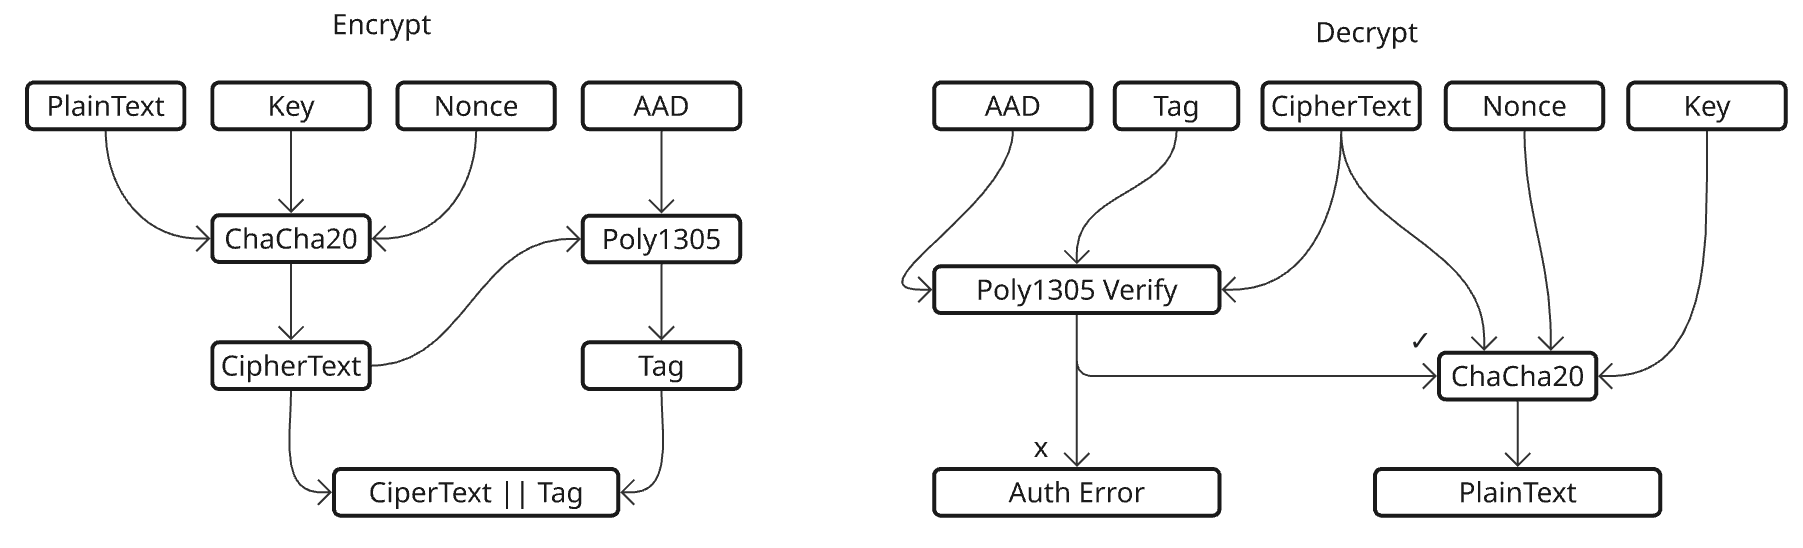
\includegraphics[width=0.82\textwidth]{plots/fig_aead_flow.png}
\caption{ChaCha20-Poly1305 AEAD: tok šifrovania (vľavo) a dešifrovania (vpravo).
Poly1305 autentifikuje AAD aj CipherText spoločne.
Pri dešifrovaní sa overenie tagu vykoná \emph{pred} dešifrovaním.}
\label{fig:aead_flow}
\end{figure*}

\subsubsection{ChaCha20-Poly1305, XChaCha20-Poly1305 a nonce manažment}

AEAD konštrukcie sú \uv{krehké} voči zneužitiu nonce: opakovanie nonce pod rovnakým kľúčom môže viesť k vážnym únikom informácií. XChaCha20-Poly1305 rozširuje nonce na 192 bitov, čo umožňuje bezpečnejšie používanie náhodných nonce pre dlhodobo žijúce kľúče\cite{XChaChaDraft,LibsodiumXChaChaDoc}. ChaCha20-Poly1305 IETF (RFC 8439) používa 96-bitový nonce s nižším bezpečným limitom pri náhodnom generovaní (${\sim}2^{48}$ správ)\cite{RFC8439}. V prototypovej implementácii sú podporené obe varianty, pričom nonce môže byť generovaný náhodne alebo deterministicky cez HMAC --- porovnanie oboch prístupov je predmetom experimentov.

\subsubsection{Associated Data (AAD)}

AEAD podporuje \emph{Associated Authenticated Data} (AAD): dáta, ktoré sa nešifrujú, ale ich integrita je kryptograficky chránená. V prístupovom protokole je AAD použité pre hlavičku frame. Tým sa zabezpečí, že zmena \texttt{reader\_id}, \texttt{door\_id} alebo \texttt{seq} spôsobí zlyhanie overenia tagu.

\subsubsection{Porovnanie s AES-GCM}

AES-GCM (Galois/Counter Mode) je dominantnou AEAD konštrukciou v TLS~1.3 a podnikových systémoch\cite{RFC8446}. Pre kontext tejto práce je relevantné porozumieť, prečo bol zvolený ChaCha20-Poly1305 namiesto AES-GCM.

\begin{table}[htbp]
\renewcommand{\arraystretch}{1.3}
\centering
\caption{Porovnanie ChaCha20-Poly1305 a AES-GCM}
\label{tab:chacha-vs-aesgcm}
\small
\begin{tabular}{p{3.2cm} p{4.5cm} p{4.5cm}}
\toprule
\textbf{Vlastnosť} & \textbf{ChaCha20-Poly1305} & \textbf{AES-GCM} \\
\midrule
Veľkosť nonce & 96~b (IETF) / 192~b (XChaCha20) & 96~b \\
Nonce reuse & Únik XOR plaintextov (two-time pad) & Kritické: extrahovateľný GHASH kľúč\cite{RFC5116} \\
Softvér bez HW & Konštantný čas (ARX)\cite{Bernstein2012} & Timing side-channel bez AES-NI \\
HW akcelerácia & AVX2/SSSE3 (SIMD) & AES-NI (Intel/ARM) \\
Vhodnosť pre IoT & Vysoká & Iba s HW akcelerátorom \\
Štandardizácia & RFC~8439, TLS~1.3 & RFC~5116, TLS~1.3 \\
\bottomrule
\end{tabular}
\end{table}

Kľúčovým rozdielom pre softvérové nasadenie je bezpečnosť implementácie bez hardvérovej podpory. AES pracuje so S-boxom, ktorého tabuľkové implementácie vykazujú závislosti na vstupe v čase prístupu do cache --- tzv.\ \emph{cache timing} útok\cite{Bernstein2012}. ChaCha20 je čistá ARX konštrukcia bez tabuľkových vyhľadávaní, kde sú všetky operácie identicky časované.

Rozdiel pri zneužití nonce je obzvlášť dôležitý: pri AES-GCM vedie opakovaný nonce k tzv.\ \emph{forbidden attack}, kde zo dvoch šifrovaných textov pod rovnakým nonce a kľúčom možno analyticky extrahovať hodnotu použitú v GHASH a kovať MAC tagy pre ľubovoľné správy\cite{RFC5116}. Pri ChaCha20-Poly1305 vedie nonce reuse k úniku XOR plaintextov, čo je vážne, ale Poly1305 kľúč $r$ zostáva neodhalený --- degradácia bezpečnosti je teda iného charakteru.

Pre prototyp nasadzovaný na ESP32 (bez AES-NI) je ChaCha20-Poly1305 konzistentne bezpečná voľba bez platformovej závislosti.

\subsection{Náhodnosť, nonce a praktické generovanie}

Mnohé bezpečnostné protokoly stoja na predpoklade, že niektoré hodnoty sú nepredvídateľné (napr. nonce, kľúče). V embedded prostredí však môže byť generovanie kvalitnej náhodnosti problematické: zariadenie nemusí mať dostatok entropie a môže sa spoliehať na deterministické zdroje. Existujú tri základné stratégie generovania nonce:

\begin{itemize}[leftmargin=*,itemsep=2pt]
  \item \textbf{Náhodný nonce} --- jednoduchý, ale závisí na kvalite RNG a pri krátkom nonce (96 bitov u ChaCha20) hrozí kolízia pri vysokom počte správ.
  \item \textbf{Deterministický nonce (HMAC)} --- nonce sa odvodí ako $\text{HMAC}(K_{\text{nonce}}, \text{context})$, kde kontext zahŕňa hlavičku správy. Eliminuje závislosť na RNG, ale vyžaduje zdieľanie nonce kľúča medzi odosielateľom a overovateľom.
  \item \textbf{Deterministický nonce s runtime verifikáciou} --- rovnaký HMAC nonce, ale server navyše overuje, že prijatý nonce zodpovedá očakávanej hodnote. Ak nezodpovedá, zariadenie sa zakaranténuje.
\end{itemize}

Rozšírený nonce pri XChaCha20-Poly1305 znižuje riziko kolízie aj pri náhodných noncoch\cite{LibsodiumXChaChaDoc}, čo je výhodné v systémoch s dlhšou životnosťou kľúčov. Deterministický HMAC nonce túto výhodu posúva ešte ďalej: pri správnej konštrukcii sa nonce neopakuje ani pri chybnom RNG.

\subsection{Domain separation a kontext v derivácii kľúčov}

Aj keď je HKDF formálne jednoduchý, v praxi je kľúčové správne nastaviť \emph{context/label} (parameter \texttt{info}). Domain separation znamená, že z rovnakého master secret sa odvodia rôzne podkľúče tak, aby sa nedali zameniť. Typickým prístupom je použiť popis účelu, napríklad \texttt{"hw-auth"}, \texttt{"aead-frame"} alebo \texttt{"audit-chain"}. Takéto označovanie je jednoduché, ale výrazne znižuje riziko, že sa jeden kľúč \uv{nechtiac} použije inde.

\subsection{Kryptografia vs. bezpečnosť implementácie}

Bezpečnosť algoritmov môže byť oslabená implementáciou. Typické chyby sú porovnávanie MAC ne-konštantným časom, únik citlivých údajov do logov, neobmedzené spracovanie veľkých vstupov (vyčerpanie zdrojov) a nedostatočné ošetrenie chýb. Preto sa v bezpečnom návrhu uplatňuje zásada: primitíva sú nutné, ale nestačia. Rovnako dôležité je robustné spracovanie vstupov, limity a jednotné chybové správanie.

\subsection{Bezpečnostné modely AEAD a nonce-misuse resistance}

Porozumenie formálnym bezpečnostným modelom pomáha presne formulovať, čo zaručujú kryptografické protokoly a kde sú hranice ich bezpečnosti.

\paragraph{Štandardný model (nAE).}
AEAD bezpečnosť sa formálne definuje dvoma vlastnosťami\cite{RFC5116}:
\begin{itemize}[leftmargin=*,itemsep=2pt]
  \item \textbf{IND-CPA} (Indistinguishability under Chosen-Plaintext Attack): šifrovaný text je nerozoznateľný od náhodných dát aj keď útočník môže vybrať plaintexty.
  \item \textbf{INT-CTXT} (Integrity of Ciphertext): útočník nedokáže skovať platný šifrovaný text s platným tagom, ani pri adaptívnych dotazoch na šifrovaní.
\end{itemize}
Kombinácia IND-CPA + INT-CTXT tvorí \emph{AE} bezpečnosť --- presne to, čo poskytujú ChaCha20-Poly1305 a XChaCha20-Poly1305 pri unikátnych nonce\cite{RFC8439}. Štandardný model (\emph{nonce-based AE}, nAE) predpokladá, že nonce sa neopakuje. Porušenie tohto predpokladu degraduje bezpečnostné záruky spôsobom závislým od konkrétnej konštrukcie.

\paragraph{Nonce-misuse resistance.}
Rogaway a Shrimpton\cite{RogawayNonceMisuse2004} formalizovali silnejší model, kde šifra zachováva \emph{dôvernosť} aj pri opakovanom nonce --- za cenu, že útočník rozpozná zhodné plaintexty pri rovnakom nonce. Konštrukcie dosahujúce tento cieľ (napr.\ SIV alebo DAE)\cite{BellareNonceMisuse2006} vyžadujú spravidla dva priechody správou.

Táto práca nepoužíva nonce-misuse resistant primitívum, ale namiesto toho kompenzuje na protokolovej úrovni: profily R1/R2 používajú deterministický HMAC nonce odvodený z kontextu vrátane unikátneho \texttt{seq} --- nonce sa neopakuje, kým sa neopakuje celý kontext. Profil R2 navyše aktívne detekuje nonce mismatch na serveri a zakaranténuje zariadenie. Ide o praktický kompromis: zachováva nAE primitívum (bez overhead SIV), ale znižuje riziko zneužitia nonce prostredníctvom deterministickej konštrukcie a serverovej verifikácie\cite{RogawayNonceMisuse2004,BellareNonceMisuse2006}.


% ==============================================================

% ==============================================================
\section{Zásady návrhu bezpečných protokolov}

Pri čítaní bezpečnostnej literatúry je ľahké nadobudnúť dojem, že rozhoduje najmä výber algoritmu. Pri praktickom protokole to tak nebýva. O výsledku často rozhodne obyčajná vec: nejednoznačný formát, nevhodná chybová hláška alebo príliš dôverčivý parser. Preto má táto kapitola možno menej \uv{kryptografický} charakter, ale pre výslednú bezpečnosť je rovnako dôležitá.

\subsection{Fail-closed správanie}

Pri prístupovom systéme býva prirodzené pýtať sa, ako zabezpečiť, aby sa dvere otvorili vždy, keď majú. Bezpečnostný návrh si však musí rovnako tvrdo položiť opačnú otázku: čo sa stane, keď si systém nie je istý? V tejto práci je odpoveď jednoznačná. Ak zlyhá HMAC, validácia vstupu, anti-replay alebo interná konzistencia dát, výsledkom nie je \uv{skúsme to ešte nejako zachrániť}, ale zamietnutie. Takýto prístup je menej pohodlný pri ladení, no bezpečnejší v prevádzke.

\subsection{Jednoznačná serializácia a kanonizácia}

Pri podpisovaní alebo šifrovaní je kritické, aby všetky strany pracovali s rovnakou reprezentáciou dát. Ak by napríklad hardvér podpisoval JSON s iným poradím polí než server, mohlo by dôjsť k chybnému odmietnutiu. Naopak, ak by server akceptoval viacero reprezentácií, útočník môže hľadať \emph{gadgety} na bypass podpisu. Preto prototyp podpisuje \emph{raw body} a server používa rovnaký presný vstup do HMAC.

\subsection{Verzovanie formátu a algoritmov}

Bezpečné systémy musia počítať s evolúciou: zmeny formátu, rotácia kľúčov, prípadne migrácia algoritmov. Preto protokol obsahuje polia ako \texttt{key\_version} a interné limity (maximálne dĺžky polí, verzovanie), čo znižuje riziko \uv{tichých} nekompatibilít.


\subsection{Bezpečné spracovanie chýb a jednotné odpovede}

Chybové správy sú často podceňovaný komunikačný kanál. Ak systém vracia detailné dôvody zlyhania (napr. \uv{nesprávny podpis}, \uv{neznáma čítačka}, \uv{príliš staré seq}), útočník môže tieto informácie využiť na \emph{enumeráciu} a postupné zlepšovanie útoku. Zároveň však prevádzka potrebuje vedieť, čo sa deje. Rozumný kompromis je: jednotná odpoveď smerom k nedôveryhodnému klientovi a detailný dôvod iba v internom logu a administrácii.

\subsection{Ochrana proti DoS a vyčerpaniu zdrojov}

DoS (Denial of Service) je relevantný aj pre prístupové scenáre, pretože môže spôsobiť výpadok vstupov alebo núdzový režim. Na úrovni protokolu a servera je vhodné uplatniť limity veľkosti požiadaviek, rýchlu validáciu pred náročnými operáciami (napr. pred dešifrovaním), a jednoduché ochrany proti floodu (rate limiting). Takéto opatrenia nezrušia DoS úplne, ale zvyšujú odolnosť.

\subsection{Bezpečnosť knižníc a závislostí}

Kryptografické primitíva je vhodné realizovať cez overené knižnice. Z teoretického hľadiska to znamená minimalizovať \uv{vlastnú kryptografiu}, sledovať aktualizácie a mať testy, ktoré zachytia regresie. V prototypovej implementácii je kryptografická vrstva postavená na knižnici libsodium.\cite{LibsodiumXChaChaDoc}

\subsection{Mapovanie bezpečnostných cieľov na mechanizmy}

Tabuľka \ref{tab:security-mapping} sumarizuje, ktorý mechanizmus v prototypovom systéme poskytuje akú bezpečnostnú vlastnosť.

\begin{table}[h]
\renewcommand{\arraystretch}{1.3}
\centering
\begin{tabular}{@{}ll@{}}
\toprule
Bezpečnostná vlastnosť & Mechanizmus v prototypu \\
\midrule
Autentickosť požiadavky od HW & HMAC-SHA-256 nad HTTP požiadavkou \\
Integrita metadát (reader/door/seq) & AEAD AAD väzba hlavičky frame \\
Dôvernosť interného payloadu & AEAD ChaCha20/XChaCha20-Poly1305 \\
Ochrana proti replay & hw\_seq + ReplayWindow (sliding window) \\
Súkromie identifikátora v DB & HMAC(card\_id) s pepper \\
Detekcia manipulácie auditu & HMAC hash chain + audit anchor \\
\bottomrule
\end{tabular}
\caption{Mapovanie bezpečnostných cieľov na mechanizmy v prototypovom systéme}
\label{tab:security-mapping}
\end{table}

\section{Správa kryptografických kľúčov}

V prototypoch sa o kľúčoch často píše iba jednou vetou: \uv{uložia sa do konfigurácie}. To síce môže byť pravda, ale z bezpečnostného pohľadu to nič nevysvetľuje. Aj jednoduchý systém potrebuje vedieť, odkiaľ sa kľúče berú, na čo presne slúžia, kedy sa menia a čo sa stane po incidente. NIST SP 800-57 tento problém opisuje ako životný cyklus kľúča\cite{NIST80057}; v praxi je to skôr séria nepríjemných, ale nevyhnutných prevádzkových otázok.

\subsection{Oddelenie kľúčov podľa účelu}

Dobrá prax je používať odlišné kľúče pre odlišné účely:

\begin{itemize}[leftmargin=*,itemsep=2pt]
  \item kľúč pre HW autentifikáciu (HMAC podpis HTTP),
  \item kľúč pre AEAD šifrovanie payloadu,
  \item kľúč pre audit hash chain,
  \item \emph{pepper} pre hashovanie identifikátorov kariet.
\end{itemize}

Použitie jedného kľúča pre viac účelov môže viesť k \emph{cross-protocol} útokom alebo k nejasnostiam pri rotácii. Preto je vhodné odvodiť podkľúče z hlavného tajomstva pomocou HKDF\cite{RFC5869}.

\subsection{Verzovanie a rotácia kľúčov}

V prototypovej implementácii má čítačka priradenú \texttt{key\_version}. Pri rotácii sa v databáze nastaví nová verzia a server môže dočasne akceptovať aj predchádzajúcu verziu (\emph{allow-previous}), aby sa minimalizoval výpadok pri prechode.

\subsection{Ukladanie kľúčov a bezpečnosť servera}

Kľúče sú v prototypovej verzii uložené v konfiguračnom súbore servera (ako hex reťazce) a načítané pri štarte. Ide o pragmatické riešenie vhodné pre experimentálny prototyp, no z pohľadu produkčnej bezpečnosti predstavuje vedomý kompromis. V produkčnom nasadení by bolo vhodné použiť dedikované úložisko tajomstiev (napr. HSM, Vault), obmedziť prístupové práva procesu a oddeliť správu tajomstiev od aplikačného servera.

\subsection{Provisioning a registrácia zariadení}

V produkčnom systéme je dôležitá fáza provisioningu: ako sa čítačka prvýkrát dostane do systému a ako sa jej priradia tajomstvá. Teoreticky existujú dva prístupy: predzdieľané tajomstvo (PSK) vložené pri výrobe/inštalácii alebo bootstrap protokol (napr. na báze certifikátov). PSK je jednoduchšie, ale horšie škáluje a vyžaduje disciplinované nakladanie s tajomstvom počas celej životnosti zariadenia.

\subsection{Kompromitácia kľúča a postup obnovy}

Aj pri dobrej implementácii treba počítať s kompromitáciou zariadenia alebo únikom kľúča. Incident plán by mal riešiť, ako rýchlo vieme zablokovať kompromitované zariadenie, ako prebehne rotácia kľúčov a ako identifikujeme udalosti, ktoré mohli byť ovplyvnené kompromitáciou.

\subsection{Evidencia verzií a migračné stratégie}

Migrácia bezpečnostných mechanizmov je citlivá, pretože výpadok znamená praktický problém v prevádzke. Z teoretického hľadiska sa často používa fázovaný rollout, krátke obdobie dual-acceptance (prijíma sa stará aj nová verzia) a následná revokácia starších verzií.


Pre digitálne identity a autentifikátory sú relevantné aj odporúčania NIST SP 800-63-4, ktoré zdôrazňujú riadenie autentifikátorov, životný cyklus a procesy obnovy.

% ==============================================================
\section{Návrh bezpečného komunikačného protokolu}

Bezpečnostné princípy z predchádzajúcich kapitol sa musia premietnuť do konkrétneho protokolu, ktorý bude fungovať v reálnych podmienkach. Táto kapitola popisuje tok spracovania udalosti, formát správ a kľúčové dizajnové rozhodnutia, ktoré sú základom pre implementovaný prototyp.

\subsection{End-to-end tok udalosti}

V tejto práci sa z bezpečnostného hľadiska oplatí sledovať udalosť od úplného začiatku. Čítačka prečíta UID, zariadenie zvýši \texttt{hw\_seq}, vytvorí krátku HTTP požiadavku a podpíše ju. Server po prijatí ešte stále \uv{nepovoľuje vstup}; najskôr overí pôvod a základnú konzistenciu správy. Až potom sa z požiadavky vytvorí interný secure frame, ktorý vstupuje do rozhodovacej logiky.

Prakticky teda tok vyzerá takto:
\begin{enumerate}[leftmargin=*,itemsep=2pt]
  \item RC522 načíta UID karty.
  \item ESP32 inkrementuje perzistentné \texttt{hw\_seq}.
  \item Do \texttt{/api/hw/uid} sa odošle JSON s \texttt{uid}, \texttt{reader\_id}, \texttt{door\_id} a \texttt{hw\_seq}.
  \item Hlavička \texttt{X-HW-Signature} nesie HMAC nad presným telom požiadavky.
  \item Server overí podpis a validuje vstup.
  \item Zo správy vytvorí interný frame, kde sa \texttt{hw\_seq} použije ako \texttt{seq}.
  \item \emph{DecisionEngine} vyhodnotí pravidlá a výsledok sa uloží do auditu.
  \item EventBus sprístupní runtime udalosti pre administráciu.
\end{enumerate}

Takéto rozdelenie vrstiev je dôležité aj pri interpretácii výsledkov. HMAC medzi zariadením a serverom rieši autenticitu a integritu požiadavky. AEAD frame na serverovej strane potom rieši vnútorné spracovanie, väzbu metadát a auditovateľnosť ďalších krokov.

\subsection{Formát správ, validácia vstupu a obrana pred parser útokmi}

V prístupovom systéme predstavuje vstupná správa (napr. JSON požiadavka) hranicu medzi nedôveryhodným svetom a internou logikou servera. Aj keď je správa podpísaná, server musí počítať s tým, že útočník sa môže pokúsiť o:

\begin{itemize}[leftmargin=*,itemsep=2pt]
  \item poslať extrémne veľké alebo špeciálne formátované vstupy (vyčerpanie pamäte),
  \item využiť rozdiely v parsovaní (napr. rozdiel medzi \uv{číslo} a \uv{reťazec}),
  \item obísť kontrolu pomocou duplicitných polí alebo neštandardných kódovaní.
\end{itemize}

Z teoretického hľadiska sa odporúča spracovať vstup v dvoch krokoch:

\begin{enumerate}[leftmargin=*,itemsep=2pt]
  \item syntaktická validácia (správny JSON, maximálna veľkosť, povolené znaky),
  \item semantická validácia (povinné polia, rozsahy hodnôt, typy, konzistentnosť).
\end{enumerate}

Až po úspešnej validácii má zmysel vykonávať ďalšie operácie (napr. dešifrovanie, databázové dotazy). Tento postup znižuje riziko DoS a zlepšuje robustnosť.

\subsection{Hranice dôvery a spracovanie metadát}

Nie všetky polia v správe majú rovnaký význam. Napríklad \texttt{uid} je identifikátor karty, no nie je dôkazom autenticity. Naopak \texttt{reader\_id} a \texttt{door\_id} sú metadáta, ktoré určujú kontext autorizácie a musia byť chránené proti manipulácii. V návrhu je dôležité definovať, ktoré polia sa:

\begin{itemize}[leftmargin=*,itemsep=2pt]
  \item považujú za nedôveryhodné a slúžia iba ako vstup do politiky,
  \item musia byť kryptograficky viazané (napr. cez HMAC alebo AEAD AAD),
  \item musia byť odvodené na serveri (napr. časová pečiatka).
\end{itemize}

Takéto rozdelenie znižuje riziko, že server začne dôverovať údajom, ktoré útočník vie ovplyvniť.

\subsection{Škálovanie anti-replay pri viacerých zariadeniach}

Anti-replay mechanizmus musí byť v praxi navrhnutý tak, aby fungoval pre viac zariadení súčasne. To znamená, že \texttt{ReplayWindow} sa typicky udržiava per identitu zariadenia (napr. per \texttt{reader\_id}). Pri návrhu je potrebné rozhodnúť:

\begin{itemize}[leftmargin=*,itemsep=2pt]
  \item aká je veľkosť okna (koľko hodnôt tolerujeme),
  \item či tolerujeme out-of-order doručenie (napr. pri výpadkoch siete),
  \item a ako riešime reštart zariadenia alebo stratu stavu.
\end{itemize}

Z teoretického hľadiska je vhodné, aby server odmietol nečakaný pokles sekvencie, ale zároveň poskytol administrátorovi diagnostiku (napr. zariadenie bolo resetované). Vtedy je možné zvoliť bezpečný proces obnovy (napr. re-provisioning alebo manuálne potvrdenie resetu).

\subsection{Časové okná, oneskorenie a \uv{freshness}}

Ak sa používa časová pečiatka, treba počítať s oneskorením siete a s tým, že klient nemusí mať presný čas. Praktický prístup je, že server generuje čas pre interné správy a pri príjme požiadavky používa čas iba pre audit a pre detekciu anomálií (napr. nezvyčajne dlhé oneskorenie). Ak sa predsa používa klientsky čas, musí existovať tolerancia (maximálny \emph{skew}) a fail-closed správanie mimo tolerancie.

\subsection{Autentifikácia hardvéru cez HMAC}

HMAC podpis požiadavky zabezpečuje, že iba zariadenie s tajným kľúčom vie vytvoriť platnú požiadavku. To bráni podvrhnutiu (spoofing). V prototypovej architektúre je dôležité, že zariadenie nepoužíva administrátorský token (ten je určený iba pre UI), čo znižuje riziko zneužitia v prípade kompromitácie zariadenia.

\subsection{Anti-replay: sekvencie a \emph{ReplayWindow}}

\subsubsection{Prečo je replay útok nebezpečný}

Replay útok je praktický najmä tam, kde je výsledok udalosti deterministický (napr. \emph{ALLOW}) a útočník vie zachytiť komunikáciu. Bez anti-replay by stačilo raz zachytiť platnú požiadavku a opakovať ju.

\subsubsection{Monotónne \texttt{hw\_seq}}

Zariadenie používa monotónne sekvenčné číslo \texttt{hw\_seq}, ktoré sa inkrementuje pri každom skene a perzistentne ukladá do NVS. V prípade reštartu zariadenia sa hodnota obnoví. Monotónnosť je dôležitá: ak by sa \texttt{hw\_seq} resetoval, útočník by mohol znovu použiť staré hodnoty.

\subsubsection{Sliding window na serveri}

Server používa mechanizmus \emph{sliding window} (ReplayWindow). Udržiava:\
(1) \texttt{maxSeen} a\
(2) bitset použitia hodnôt v rozsahu \texttt{[maxSeen - window, maxSeen]}.

Ak príde \texttt{seq} príliš staré, server ho odmietne ako \emph{too old}. Ak spadá do okna, ale už bolo použité, odmietne ho ako \emph{replay}. Tento model je bežný v protokoloch, ktoré musia tolerovať out-of-order doručenie, ale zároveň odmietnuť duplicitné správy.

\subsection{Freshness a časová pečiatka}

V embedded zariadení nie je zaručená presnosť času. Preto server generuje \texttt{ts\_unix\_ms} a používa ho v hlavičke frame. Čas slúži pre audit, pre detekciu anomálií a pre \emph{freshness} logiky (napr. maximálne povolené oneskorenie správy).

\subsection{Poznámka k dôvernosti komunikácie}

V prototypovej implementácii je HW požiadavka autentifikovaná (integrita a pôvod), ale dôvernosť prenosu UID na úrovni HTTP nie je v základnom režime kryptograficky chránená. V praxi je vhodné použiť TLS (HTTPS) alebo posielať už šifrovaný payload z hardvéru. V tejto práci sa dôvernosť posilňuje najmä na úrovni úložiska (neukladanie surového UID) a na úrovni interného protokolu (AEAD frame), pričom absencia povinného TLS je vedomé zjednodušenie prototypu a nie deklarovaná bezpečnostná vlastnosť.


% ==============================================================
\section{Bezpečnosť vstavaného zariadenia a spracovanie tajomstiev}

Čítačka je z hľadiska bezpečnosti nepohodlný prvok. Nie je pod takou kontrolou ako server, býva fyzicky dostupná a zároveň nemá veľa výkonu ani priestoru na zložitejšie protiopatrenia. Pri návrhu preto nepomáha tváriť sa, že ide o plnohodnotne dôveryhodný uzol. Užitočnejšie je počítať s tým, že zariadenie môže byť slabším článkom a že server musí jeho správy vždy znovu overiť.

Model hrozieb preto zahŕňa situácie, v ktorých útočník získa:

\begin{itemize}[leftmargin=*,itemsep=2pt]
  \item krátkodobý fyzický prístup (napr. otvorenie krytu, pripojenie k rozhraniam),
  \item možnosť resetovať napájanie alebo opakovane reštartovať zariadenie,
  \item možnosť odoberať firmware z pamäte (v závislosti od ochrany),
  \item možnosť ovplyvniť prostredie (Wi-Fi, rušenie, pokusy o MITM).
\end{itemize}

V praxi to znamená, že zariadenie sa nemá považovať za \uv{dôveryhodné} v rovnakom zmysle ako server. Zariadenie je skôr klient, ktorého správy sa musia overiť a limitovať.

\subsection{Ukladanie tajomstiev na zariadení}

Najväčším problémom pri jednoduchých schémach je dlhodobo uložené tajomstvo (napr. PSK pre HMAC). Ak útočník tajomstvo získa, vie zariadenie plnohodnotne emulovať. Preto sa v teórii odporúča:

\begin{itemize}[leftmargin=*,itemsep=2pt]
  \item používať per-device tajomstvá (každé zariadenie má vlastný kľúč),
  \item oddeliť tajomstvá podľa účelu (autentifikácia, šifrovanie, audit),
  \item a uvažovať o hardvérových mechanizmoch (secure element, flash encryption).
\end{itemize}

V prostredí ESP32 existujú mechanizmy ako \emph{Secure Boot} a \emph{Flash Encryption}, ktoré dokážu sťažiť extrakciu firmware a tajomstiev. Pre prototyp nie je cieľom implementovať kompletný hardening, ale v teoretickej rovine je dôležité tieto možnosti poznať a zvážiť ich v produkčnom návrhu.

\subsection{Monotónne počítadlá a trvácnosť stavu}

Anti-replay mechanizmy často pracujú so sekvenčným číslom alebo časom. Aby mali význam, musia byť trvácne aj po reštarte. Z toho vyplývajú dve praktické otázky:

\begin{itemize}[leftmargin=*,itemsep=2pt]
  \item Ako ukladať stav tak, aby sa pri výpadku napájania nestratil?
  \item Ako zabrániť rollbacku stavu (útočník obnoví starú hodnotu)?
\end{itemize}

Jednoduché perzistentné ukladanie (napr. NVS) rieši prvú otázku. Druhá otázka je zložitejšia a v produkcii sa rieši napríklad cez secure storage, monotónne čítače v hardvéri alebo serverové pravidlá, ktoré odmietnu nečakaný pokles sekvencie.

\subsection{Bezpečnosť firmware a aktualizácie}

Pri mikrokontroléri býva firmware zároveň funkciou aj bezpečnostnou hranicou. Keď sa v ňom objaví chyba, nestačí povedať, že ju \uv{niekedy opravíme}; bez rozumného mechanizmu aktualizácie zostane slabé miesto v zariadení prakticky po celý jeho životný cyklus. Na druhej strane, ak sa aktualizácie navrhnú zle, stanú sa najkratšou cestou k prevzatiu zariadenia.

Preto sa v odbornej literatúre opakuje niekoľko rovnakých zásad: nový firmware má byť podpísaný, zariadenie má vedieť odmietnuť staršiu zraniteľnú verziu a vývojové rozhrania nemajú zostať otvorené v nasadení. V tejto práci nie je implementovaný plnohodnotný secure boot ani OTA aktualizácia; bolo by nepresné tvrdiť opak. Z pohľadu témy je však dôležité pomenovať, že práve firmware rozhoduje o tom, či sa zachová správne počítadlo \texttt{hw\_seq}, či sa tajomstvo použije iba na podpis a či zariadenie neposiela na sieť viac údajov, než má.

\subsection{Fyzické útoky a praktický hardening}

Keď je čítačka pri dverách fyzicky dostupná, model hrozieb sa mení. Útočník už nemusí útočiť cez sieť; môže skúšať debug port, napájanie, vnútornú zbernicu alebo jednoducho vymeniť modul za vlastný. V laboratórnom prototype sa proti takémuto súperovi nedá dosiahnuť rovnaká odolnosť ako v komerčnom kontroléri so secure elementom a chráneným krytom. Dáva preto zmysel hovoriť o primeranom hardeningu, nie o úplnej fyzickej odolnosti.

Prakticky to znamená aspoň tri veci. Po prvé, vypnúť alebo obmedziť rozhrania, ktoré boli užitočné pri vývoji, ale v prevádzke by iba rozširovali útočnú plochu. Po druhé, premýšľať nad tým, čo sa stane po kompromitácii jednej čítačky; v dobre navrhnutom systéme to nesmie automaticky znamenať kompromitáciu celej serverovej časti. A po tretie, pri interpretácii výsledkov práce otvorene priznať, že fyzická ochrana zariadenia tu nie je hlavným predmetom riešenia.

\subsection{Bezpečnosť Wi-Fi konfigurácie a lokálnej siete}

Wi-Fi býva v prototypoch často najpraktickejšia voľba, ale zároveň prináša typický problém: zariadenie sa ocitne v sieti, kde nie je samo. Vedľa neho môžu byť telefóny, notebooky aj iné IoT prvky, ktoré nemusia byť dôveryhodné. Práve preto nestačí pozerať sa iba na obsah správy; dôležité je aj to, z akej siete zariadenie komunikuje a s kým vôbec smie hovoriť.

Pre tento typ riešenia je rozumné oddeliť zariadenia aspoň do samostatnej siete alebo VLAN, zúžiť komunikáciu na nevyhnutné endpointy a nenechať otvorené všeobecné služby, ktoré prototyp nepotrebuje. Silné Wi-Fi zabezpečenie a monitorovanie neúspešných spojení sú už skôr prevádzkové disciplíny, ale v praxi často rozhodnú o tom, či incident zostane lokálny, alebo sa rozšíri ďalej. Sieťová segmentácia sama osebe kryptografiu nenahrádza; iba kupuje čas a znižuje dosah problému.

\subsection{Bezpečnosť logovania na zariadení}

Pri embedded zariadení je lákavé logovať všetko, najmä počas ladenia. Presne tu však vzniká bežná chyba: do konzoly sa dostanú informácie, ktoré tam po nasadení nemajú čo robiť. V tomto prototype majú logy slúžiť hlavne na diagnostiku čítačky a komunikácie, nie na prenos citlivých údajov. Záznamy preto nemajú obsahovať tajomstvá, celé podpisy ani zbytočne detailné vnútorné stavy.

Rovnako dôležité je, aby sa zo servisného logovania nestal trvalý režim prevádzky. To, čo pomáha pri vývoji, môže po nasadení fungovať ako jednoduchý únikový kanál. Aj pri tak malej súčasti systému sa teda ukazuje rovnaký princíp ako inde: diagnostika je potrebná, ale musí byť podriadená bezpečnostnému cieľu, nie naopak.


% ==============================================================
\section{Bezpečnosť transportnej vrstvy a použitie TLS}

Pri komunikácii medzi čítačkou a serverom sa ľahko zmiešajú dve odlišné vrstvy ochrany. Jedna otázka znie, či je dôveryhodná samotná požiadavka --- teda či server vie, kto ju vytvoril a či ju nikto po ceste neupravil. Druhá otázka sa týka celého prenosu po sieti: či niekto nevie čítať alebo meniť komunikáciu na transportnej vrstve. HMAC a AEAD riešia prvý problém na úrovni správy; TLS rieši druhý na úrovni spojenia. Obe vrstvy sú užitočné, ale ich úloha nie je zameniteľná.\cite{RFC8446,RFC9325}

\subsection{Prečo nestačí iba TLS}

Samotné TLS neodpovie na všetko. Ak je zariadenie kompromitované, vie stále vytvárať úplne korektné HTTPS požiadavky. Ak je chyba v serverovej autorizácii, TLS ju nezakryje. A ak je v architektúre prítomná proxy alebo reverzný front-end, transportná ochrana sa môže ukončiť ešte pred aplikáciou, ktorá rozhoduje o prístupe.

Preto dáva zmysel ponechať si aj aplikačnú autentifikáciu. V tomto prototype túto úlohu plní HMAC nad telom požiadavky a väzba na \texttt{hw\_seq}. Aj keby sa transportná vrstva neskôr zmenila, server stále vie overiť, že prijatá udalosť zodpovedá tomu, čo odoslalo konkrétne zariadenie.

\subsection{mTLS vs. symetrické tajomstvá}

Pri autentifikácii zariadení sa v praxi stretávajú dve cesty. Prvá je postavená na symetrickom tajomstve, z ktorého sa počíta HMAC; druhá používa certifikáty a mutual TLS. mTLS sa lepšie hodí do väčších infraštruktúr, kde treba riešiť životný cyklus identity zariadenia, revokáciu a správu certifikátov. Má však aj cenu: PKI, distribúcia dôvery a komplikovanejšie nasadenie na strane klienta.

Pre tento prototyp bol zvolený jednoduchší model so zdieľaným tajomstvom. Nie preto, že by mTLS nebolo bezpečné, ale preto, že cieľom práce nebolo stavať certifikačnú infraštruktúru. HMAC stačí na demonštráciu autenticity zariadenia, integrity požiadavky a ochrany proti replay na aplikačnej vrstve.

\subsection{Validácia certifikátu a \emph{certificate pinning}}

Ak sa TLS použije, najslabším miestom býva paradoxne klient. V embedded praxi sa stále objavujú implementácie, ktoré certifikát servera neoverujú dôsledne, alebo validáciu vypnú úplne, lebo je \uv{jednoduchšie rozbehať spojenie}. V takom prípade ostane z TLS iba šifrovaný tunel bez skutočnej identity servera.

Pre stabilné prostredia prichádza do úvahy aj \emph{certificate pinning}, teda uloženie očakávaného verejného kľúča alebo fingerprintu. Tým sa znižuje závislosť od všeobecného trust store, ale zároveň sa komplikuje rotácia certifikátu. Je to typický príklad mechanizmu, ktorý vyzerá čisto bezpečnostne, no v praxi sa rýchlo zmení na prevádzkový problém, ak sa zle naplánuje.\cite{RFC9325}

\subsection{Praktické nasadenie TLS v IoT}

V teórii sa TLS často spomína ako samozrejmá voľba. V malom IoT zariadení však za tým nasledujú konkrétne otázky: kde bude uložený CA certifikát, ako sa vyrieši jeho obmena, čo sa stane po expirácii a kto zabezpečí aktualizáciu zariadenia bez výpadku. Práve tu sa ukazuje rozdiel medzi \uv{bezpečným mechanizmom} a \uv{udržateľným nasadením}.

Z tohto dôvodu ostáva v prototype základná komunikácia hardvéru riešená ako HTTP + HMAC. Neznamená to, že TLS nie je dôležité; znamená to iba to, že ťažisko práce je inde. Produkčné riešenie by malo pridať TLS alebo mTLS aj kvôli dôvernosti prenášaného identifikátora.

\subsection{Kombinácia vrstiev: kedy dáva zmysel HMAC aj pri TLS}

Otázka \uv{prečo HMAC, keď už mám TLS?} sa objavuje prirodzene. Odpoveď závisí od toho, čo presne chceme overiť. TLS chráni spojenie medzi dvoma bodmi. HMAC v tomto návrhu viaže konkrétnu požiadavku na zariadenie a na jej obsah. To je užitočné napríklad vtedy, keď sa transportná vrstva v budúcnosti presunie na proxy, load balancer alebo iný medzičlánok.

Inými slovami: TLS by vylepšilo dôvernosť a transportnú integritu, no HMAC zostáva nositeľom aplikačnej identity zariadenia. Tieto vrstvy sa preto nevylučujú; každá rieši inú časť problému.


% ==============================================================
\section{Bezpečnosť úložiska, exportov a životný cyklus dát}

Úložisko prístupového systému má dve hlavné úlohy: udržiava konfiguráciu (karty, roly, väzby) a uchováva audit udalostí. Z toho vyplýva, že únik alebo manipulácia s úložiskom má vysoký dopad.

\subsection{Minimizácia dát a pseudonymizácia}

Princíp minimalizácie hovorí, že systém má ukladať iba to, čo potrebuje. Ukladanie HMAC(card\_id) namiesto surového UID je príkladom pseudonymizácie: záznamy nie sú priamo čitateľné bez tajomstva (pepper). To znižuje dopad úniku databázy a zároveň umožňuje systém používať (vyhľadávanie karty podľa UID prebehne tak, že sa UID prepočíta na hash).

\subsection{Export/import a integritné kontroly}

Pri administrácii sa často objaví potreba exportovať databázu alebo migrovať konfiguráciu. Export/import je však rizikový: môže obísť bežné API kontroly a v prípade neovereného importu viesť k injekcii neplatných pravidiel. Z teoretického hľadiska je preto vhodné:

\begin{itemize}[leftmargin=*,itemsep=2pt]
  \item vykonať integrity check databázy po importe,
  \item verifikovať auditnú reťaz, ak je súčasťou exportu,
  \item a auditovať samotné administrátorské operácie export/import.
\end{itemize}

\subsection{Prístupové práva k databáze a zálohovanie}

Databáza je často obyčajný súbor (pri SQLite). Z bezpečnostného hľadiska to znamená, že prístupové práva na úrovni operačného systému sú kritické: proces servera má mať práva iba na čítanie/zápis, ktoré potrebuje, a administrátorské exporty majú byť auditované. Pri zálohovaní treba myslieť na to, že záloha obsahuje rovnaké citlivé dáta ako primárna databáza.

V produkcii je vhodné uvažovať aj o šifrovaní úložiska alebo o databáze s podporou šifrovania. Šifrovanie v pokoji (at-rest) však nenahrádza auditnú integritu: útočník s právami procesu môže stále dáta meniť, preto je tamper-evident logovanie doplnkovým mechanizmom.


\subsection{Retencia a ochrana súkromia v audite}

Audit záznamy sú z pohľadu bezpečnosti užitočné, ale môžu obsahovať citlivé informácie o pohybe používateľov. V produkcii je preto potrebné definovať:

\begin{itemize}[leftmargin=*,itemsep=2pt]
  \item obdobie uchovávania (retenciu),
  \item prístupové práva k auditu,
  \item a prípadné anonymizačné alebo agregované reporty.
\end{itemize}

Tieto aspekty sú najmä procesné, ale priamo súvisia s dôveryhodnosťou systému a s právnymi požiadavkami.

% ==============================================================
\section{Ochrana súkromia identifikátorov a bezpečnosť úložiska}

Ochrana identifikátorov kariet a integrity databázy sú kľúčové aspekty, ktoré priamo ovplyvňujú dôveryhodnosť systému aj pri úniku dát. Táto kapitola analyzuje riziká spojené s ukladaním surových identifikátorov a opisuje mechanizmy pseudonymizácie implementované v prototype.

\subsection{Prečo neukladať surový UID}

UID je identifikátor, ktorý môže byť v čase stabilný a unikátny. Pri úniku databázy by bolo možné:

\begin{itemize}[leftmargin=*,itemsep=2pt]
  \item získať zoznam platných identifikátorov,
  \item korelovať pohyb používateľov podľa auditných záznamov,
  \item v niektorých prípadoch použiť UID na emuláciu/klonovanie.
\end{itemize}

Preto prototyp ukladá iba odvodenú hodnotu (HMAC hash).

\subsection{HMAC(card\_id) s \emph{pepper}}

Systém ukladá do databázy hodnotu:

\begin{equation}
\texttt{card\_hash} = \mathrm{HMAC}(\texttt{pepper}, \texttt{card\_id})
\end{equation}

kde \texttt{pepper} je tajomstvo uložené mimo databázy. Ak útočník získa SQLite súbor, bez pepper nevie efektívne zistiť pôvodné \texttt{card\_id}. Tento prístup je analogický s odporúčaním \uv{oddeliť tajomstvo od databázy}.

\subsection{Pepper vs. salt a odolnosť voči slovníkovým útokom}

Pri ochrane identifikátorov sa často spomína \emph{salt}. Salt je náhodná hodnota, ktorá sa ukladá spolu s hashom a bráni tomu, aby rovnaký vstup mal rovnaký hash. V prístupových systémoch však často chceme, aby systém vedel vyhľadávať kartu podľa UID (t. j. aby rovnaký UID viedol na rovnaký \texttt{card\_hash}). Preto sa v tejto práci používa pepper — tajomstvo, ktoré sa do databázy neukladá.

Pepper chráni proti tomu, aby útočník po úniku databázy spustil efektívny slovníkový útok nad priestorom UID. Pri niektorých typoch kariet môže byť priestor UID relatívne malý alebo štruktúrovaný; práve preto je dôležité, aby útočník nemal prístup k tajomstvu, ktoré hashovanie \uv{posilňuje}. Tento prístup je analogický k bezpečnému ukladaniu hesiel, s tým rozdielom, že tu nejde o heslo používateľa, ale o identifikátor.

\subsection{Minimalizácia údajov v audite a súkromnostné riziká}

Aj keď sa surové UID do databázy neukladá, audit môže stále obsahovať informácie, ktoré umožňujú \emph{korelovať} správanie používateľov (čas, miesto, frekvencia prístupov). Z toho vyplýva, že prístup k auditu má byť obmedzený a v produkcii je vhodné zaviesť role-based prístup k auditným záznamom, pravidlá retencie a v reportoch preferovať agregované údaje pred detailnými trasami.

\subsection{Poznámka k právnym aspektom (GDPR)}

V európskom prostredí sa pri spracovaní identifikátorov a auditných záznamov často uplatňuje GDPR. Aj keď prototyp nie je produkčný systém, teoreticky je dôležité, aby návrh rešpektoval princípy minimalizácie, účelového viazania a primeranej doby uchovávania. Hashovanie UID s pepper znižuje riziko pri úniku databázy, ale auditné záznamy stále môžu predstavovať osobné údaje v závislosti od kontextu organizácie. Preto je vhodné v praxi doplniť interné pravidlá, kto má prístup k auditu a na aký účel.


\subsection{Integrita databázy a hranice SQLite}

SQLite\cite{SQLiteSec} poskytuje transakcie, obmedzenia a \emph{integrity check}, ale nepodpisuje obsah databázy a sama osebe nerieši ani distribuovanú dostupnosť či správu prístupov vo väčšej infraštruktúre. Preto pri lokálnej manipulácii súboru nie je možné zaručiť integritu bez dodatočných mechanizmov. V prototype je táto slabina čiastočne kompenzovaná tamper-evident audit logom, pričom v práci sa otvorene uvádza, že ide o lokálne úložisko vhodné pre experimentálnu a validačnú fázu.

% ==============================================================
\section{Tamper-evident audit log}

Audit v prístupovom systéme nemá slúžiť iba na to, aby si administrátor vedel spätne pozrieť, kto prišiel ku dverám. Má byť aj zdrojom dôkazu po incidente. To mení požiadavky na jeho návrh. Nestačí, že sa udalosti zapisujú; dôležité je, aby sa dalo neskôr rozpoznať, či niekto históriu nemenil alebo neorezal. Výskum v oblasti bezpečného logovania preto zdôrazňuje detekciu manipulácie a, pri silnejších schémach, aj \emph{forward integrity}\cite{SchneierKelsey1999,NIST80092}.

\subsection{Základné typy útokov na logy}

\begin{itemize}[leftmargin=*,itemsep=2pt]
  \item Modifikácia záznamu: zmena výsledku ALLOW/DENY alebo času.
  \item Vloženie záznamu: pridanie falošnej udalosti.
  \item Vymazanie (truncation): odstránenie časti logu, typicky konca.
  \item Reorder: zmena poradia udalostí.
\end{itemize}

\subsection{Hash chain s HMAC}

Prototyp používa jednoduchú, ale účinnú konštrukciu: každý záznam obsahuje HMAC hash predošlého záznamu. Zjednodušene:

\begin{equation}
H_i = \mathrm{HMAC}(K_{audit}, \mathrm{encode}(record_i) \parallel H_{i-1})
\end{equation}

kde \(K_{audit}\) je tajný auditný kľúč. Vďaka tomu zmena ktoréhokoľvek záznamu spôsobí nekonzistenciu v následných hodnotách.

\subsection{Audit anchor a ochrana proti truncation}

Hash chain sama o sebe nezabráni útoku, pri ktorom útočník odstráni posledných \(n\) záznamov a ponechá konzistentný prefix. Preto prototyp používa audit anchor: periodicky sa ukladá hodnota \(H_i\) a index \(i\) do samostatnej štruktúry. Pri verifikácii sa kontroluje, že audit log obsahuje všetky záznamy minimálne po posledný anchor.

\subsection{Forward integrity a správa auditného kľúča}

Výskum bezpečného logovania používa pojem \emph{forward integrity}: aj keď útočník v čase $t$ získa aktuálny kľúč, nemal by byť schopný spätne upraviť staršie záznamy bez detekcie. Jednoduchý hash chain s fixným kľúčom poskytuje detekciu modifikácie, ale pri kompromitácii kľúča útočník môže vytvoriť alternatívnu históriu od miesta kompromitácie. Silnejšie konštrukcie preto používajú evolúciu kľúča (kľúč sa po každom zázname alebo po epochách aktualizuje jednosmerným spôsobom).\cite{SchneierKelsey1999}

V prototypovej práci je cieľom demonštrovať tamper-evident vlastnosti a detekciu manipulačných útokov. Pre produkčný systém by bolo vhodné zvážiť aj forward-integrity varianty a pravidlá rotácie auditného kľúča.

\subsection{Uloženie anchorov a dôveryhodný referenčný bod}

Anchor zvyšuje odolnosť proti truncation, ale vytvára otázku: \emph{kde anchor uložiť tak, aby ho útočník nevedel jednoducho prepisovať?} Teoreticky existujú možnosti: uložiť anchor mimo hlavnej databázy, replikovať anchor do externého systému alebo periodicky exportovať anchor ako \uv{checkpoint} mimo dosahu bežného procesu.

\subsection{Limity a alternatívy: Merkle stromy a verifikovateľné výňatky}

Hash chain je jednoduchý a efektívny, ale verifikácia typicky vyžaduje prejsť celý log (alebo aspoň od anchoru). Pre veľké objemy dát sa používajú aj Merkle stromy, ktoré umožňujú verifikovať vybrané výňatky bez nutnosti spracovať celé dáta. Tieto prístupy sú zložitejšie na implementáciu, ale môžu byť vhodné, ak audit rastie do veľkých rozmerov alebo ak sa vyžaduje časté overovanie.


\subsection{Verifikácia a nástroj \texttt{audit\_verify}}

Verifikácia prebieha offline alebo cez admin panel:

\begin{itemize}[leftmargin=*,itemsep=2pt]
  \item načítanie záznamov a rekonštrukcia reťaze,
  \item kontrola konzistencie \(H_i\),
  \item kontrola anchor proti truncation,
  \item reportovanie prvého indexu, kde reťaz zlyhá.
\end{itemize}

% ==============================================================





% ==============================================================
\section{Odporúčania a štandardy relevantné pre návrh}

Pri návrhu bezpečnostných mechanizmov je dôležité opierať sa o etablované odporúčania a štandardy. Táto kapitola sumarizuje hlavné zdroje odporúčaní relevantné pre tento prototyp a popisuje, ako sú zohľadnené v návrhu.

\subsection{Kryptografické a protokolárne štandardy}

Kryptografická vrstva prototypu stojí na štandardizovaných primitívach. HMAC-SHA-256 je špecifikovaný vo FIPS 198-1\cite{FIPS1981} a RFC 2104\cite{RFC2104}; HKDF je definovaný v RFC 5869\cite{RFC5869}; ChaCha20-Poly1305 a XChaCha20-Poly1305 vychádzajú z RFC 8439\cite{RFC8439} a Internet-Draftu XChaCha\cite{XChaChaDraft}. Voľba štandardizovaných algoritmov namiesto vlastných konštrukcií je základnou bezpečnostnou zásadou: implementácie štandardizovaných primitív sú externe auditované, výskumná komunita ich aktívne preveruje a aktualizácie sa riadia jasným štandardizačným procesom.

Pre komunikačný protokol je kľúčovým referenčným dokumentom RFC 5116\cite{RFC5116}, ktorý definuje všeobecné rozhranie pre AEAD konštrukcie vrátane ich sémantiky bezpečnosti. Použité konštrukcie sú s týmto rozhraním kompatibilné, čo umožňuje migráciu na iný algoritmus bez zmeny protokolárnej logiky. TLS 1.3 (RFC 8446)\cite{RFC8446} a odporúčania pre jeho bezpečné nasadenie (RFC 9325)\cite{RFC9325} sú referenčnými dokumentmi pre transportnú vrstvu; hoci prototyp nepoužíva TLS v základnom režime, návrh je pripravený na jeho doplnenie.

\subsection{Bezpečnostné odporúčania pre systémy}

NIST SP 800-57\cite{NIST80057} definuje odporúčaný životný cyklus kryptografických kľúčov vrátane oddelenia kľúčov podľa účelu, verziovania a plánovanej rotácie. V prototype je tento princíp realizovaný cez HKDF deriváciu s domain separation: pre AEAD šifrovanie, nonce generovanie, pepper identifikátorov a audit HMAC existujú nezávislé podkľúče s explicitnými \texttt{info} reťazcami.

NIST SP 800-98\cite{NIST80098} sa priamo venuje bezpečnosti RFID systémov a odporúča kombináciu vrstiev ochrany: autentifikáciu zariadení, ochranu komunikácie na aplikačnej vrstve a auditovateľnosť udalostí. Tieto tri aspekty sú jadrom navrhnutého prototypu --- HMAC autentifikácia zariadenia, AEAD frame ochrana a tamper-evident audit zodpovedajú odporúčanej stratégii vrstvenia.

NIST SP 800-63B-4\cite{NIST80063B4} pokrýva digitálnu identitu a autentifikáciu. Pre prototyp je relevantný najmä princíp oddelenia autentifikácie zariadenia (HMAC) od autorizácie prístupu (RBAC). NIST SP 800-92\cite{NIST80092} definuje odporúčania pre správu bezpečnostných logov vrátane integrity záznamu a ochrany pred modifikáciou --- priama motivácia pre tamper-evident audit log v prototype.

\subsection{Súlad prototypu s odporúčaniami}

Cieľom nie je odcitovať štandardy, ale použiť ich ako rámec pre overenie návrhových rozhodnutí. Všetky kľúčové mechanizmy prototypu --- oddelenie kľúčov podľa účelu, rotácia, dôsledná validácia vstupov, fail-closed správanie a minimalizácia dôvery v klienta --- vychádzajú z princípov etablovaných v uvedených štandardoch. Oblasti, kde prototyp závedome nepokrýva plnú produkčnú úroveň odporúčaní (absencia TLS, lokálna SQLite databáza, experimentálna správa tajomstiev), sú v práci explicitne pomenované ako vedomé obmedzenia s cieľom zachovať experimentálnu reprodukovateľnosť.

% ==============================================================
\section{Riadenie rizika a návrh protiopatrení}

Pri hodnotení navrhnutého systému nie je užitočné tváriť sa, že všetky hrozby majú rovnakú váhu. V malej laboratórnej zostave je realistickejšie riešiť replay, podvrhnutie požiadavky alebo úpravu auditu než napríklad veľmi sofistikované fyzické útoky na kartu. Táto kapitola preto neponúka univerzálny katalóg rizík, ale skôr vysvetľuje, prečo boli vybrané práve tie protiopatrenia, ktoré dávajú zmysel pre tento prototyp.

\subsection{Pravdepodobnosť a dopad}

Pri hodnotení rizika sa používa matica pravdepodobnosť$\times$dopad. Napríklad replay útok je často pravdepodobný (stačí odpočúvanie siete) a jeho dopad môže byť vysoký (neoprávnený vstup). Naopak, niektoré fyzické útoky na RFID môžu mať nižšiu pravdepodobnosť v kontrolovanom prostredí, ale stále sa oplatí ich zvážiť.

\subsection{Vrstvené zabezpečenie (defense-in-depth)}

Vrstvené zabezpečenie znamená, že systém nestojí na jednom mechanizme. V návrhu sa to prejavuje tak, že HMAC chráni pôvod požiadavky,\cite{FIPS1981} anti-replay chráni pred opakovaním, AEAD chráni interné správy a integritu metadát\cite{RFC8439,LibsodiumXChaChaDoc} a tamper-evident audit log chráni dôveryhodnosť histórie.\cite{SchneierKelsey1999}

\subsection{Bezpečnosť ako proces}

Bezpečnosť nie je jednorazová vlastnosť, ale proces: zahŕňa aktualizácie, rotáciu kľúčov, revíziu pravidiel, monitoring a reakciu na incidenty. Teoretická časť preto zdôrazňuje aj prevádzkové aspekty, nielen kryptografické primitíva.

\subsection{Predpoklady a zvyškové riziko}

Každý návrh implicitne stojí na predpokladoch. V tejto práci sa typicky predpokladá, že server je lepšie chránený než čítačka a že administrátorské rozhranie je prístupné iba autorizovaným osobám. Aj pri splnení predpokladov však ostáva zvyškové riziko (residual risk), napríklad kompromitácia jednej čítačky alebo dlhodobý DoS. Dôležité je, aby systém v takom prípade zlyhal bezpečne (fail-closed) a poskytol auditné stopy pre analýzu.

\subsection{Komunikačné kompromisy a použiteľnosť}

Prístupové systémy musia byť použiteľné: rýchla odozva, nízky počet falošných zamietnutí a jednoduchá správa oprávnení. To vytvára kompromisy. Napríklad príliš úzka anti-replay \emph{window} môže spôsobovať zamietnutia pri nestabilnej sieti; príliš široká window zas znižuje bezpečnosť. Teoreticky je vhodné tieto parametre odvíjať od prostredia a mať možnosť ich meniť bez zásahu do protokolu (konfigurácia na serveri).

% ==============================================================
\section{Bezpečnosť administrátorského rozhrania a prevádzkové aspekty}

Okrem samotného protokolu je v prístupových systémoch kritické aj administrátorské rozhranie a prevádzkové procesy. Administrácia spravuje roly, väzby, karty a často umožňuje export alebo diagnostiku. Z toho vyplýva, že musí byť chránená silnejšie než bežné klienty.

\subsection{Typické webové hrozby: XSS, CSRF a spracovanie vstupu}

Administrátorské rozhranie je webová aplikácia a dedí typické webové hrozby. Aj keď ide o interné UI, zraniteľnosti ako \emph{XSS} (Cross-Site Scripting) alebo \emph{CSRF} (Cross-Site Request Forgery) môžu viesť k tomu, že útočník vykoná administrátorské operácie bez vedomia používateľa. Z teoretického hľadiska je preto vhodné:

\begin{itemize}[leftmargin=*,itemsep=2pt]
  \item sanitizovať a escapovať výstupy v UI,
  \item používať CSRF tokeny pri stavových operáciách,
  \item validovať vstupy aj v administrátorských endpointoch (nie iba na HW endpointoch).
\end{itemize}

Pri vývoji je bežné zobrazovať logy a audit v reálnom čase. Práve tu sa často objavia XSS riziká, ak sa zobrazujú nesanitizované reťazce pochádzajúce z vonkajších vstupov.


\subsection{Autentifikácia administrátora a správa relácií}

Administrátorské rozhranie by malo používať silnú autentifikáciu (ideálne viacfaktorovú), obmedzenú platnosť tokenov a bezpečné ukladanie relácií. Pri citlivých operáciách je vhodné vyžadovať opätovné overenie alebo rotáciu relácie.

\subsection{Autorizácia operácií a audit administrácie}

Operácie typu \emph{pridať kartu}, \emph{zmeniť rolu} alebo \emph{zmeniť väzbu čítačka$\rightarrow$dvere} majú priamy dopad na bezpečnosť. Preto je vhodné mať oddelené administrátorské roly a logovať administrátorské zmeny do auditnej stopy.

\subsection{Bezpečnostná konfigurácia a minimalizácia \uv{debug} rozhraní}

Debug endpointy a vývojové nastavenia sú častým zdrojom incidentov. Z teoretického hľadiska platí, že musia byť v produkcii vypnuté alebo striktne obmedzené. OWASP API Security Top 10 upozorňuje najmä na \emph{Security Misconfiguration}.\cite{OWASPAPI2023}

\subsection{Monitoring a detekcia anomálií}

Monitorovanie je doplnkom ku kryptografii: nárast \emph{HMAC fail}, \emph{replay} udalostí alebo zlyhaní verifikácie auditu môže indikovať útok alebo chybu konfigurácie. Dobre navrhnutý systém umožní nielen odmietnuť podozrivú požiadavku, ale aj poskytnúť podklady pre analýzu a zlepšenie politiky.


% ==============================================================
\section{Súvisiace prístupy a typické architektúry systémov kontroly prístupu}

Nie všetky prístupové systémy vyzerajú rovnako a nebolo by správne predstavovať navrhnutý prototyp ako jediný rozumný model. Táto kapitola preto slúži skôr na zasadenie riešenia do kontextu. Ukazuje, kde sa náš prototyp podobá bežným architektúram a kde je naopak zjednodušený práve preto, že ide o akademický a experimentálny systém.

\subsection{Centralizované vs. distribuované rozhodovanie}

Pri porovnávaní architektúr je najpraktickejšie položiť si jednoduchú otázku: kde sa prijíma rozhodnutie o otvorení dverí? V centralizovanom modeli sa udalosť pošle na server, ktorý pozná pravidlá, stav systému aj auditný kontext. To zjednodušuje správu oprávnení a revokácií, ale systém sa stáva citlivejší na výpadok siete alebo servera.

Distribuované riešenie posúva časť logiky bližšie k dverám. Výhodou je vyššia autonómia pri výpadku konektivity. Cena za to je menej pohodlná správa politiky, viac lokálnych tajomstiev a väčšia dôležitosť fyzickej bezpečnosti edge zariadenia. V praxi preto mnohé systémy skončia niekde medzi týmito pólmi: rozhodovanie je čiastočne lokálne, ale audit, konfigurácia a správa identít zostávajú centralizované.

\subsection{Online vs. offline režim a bezpečnostné kompromisy}

Offline režim pôsobí na prvý pohľad lákavo, pretože dvere \uv{fungujú aj bez siete}. Lenže práve vtedy sa ukáže, čo všetko musí vedieť samotné zariadenie: uchovávať lokálne kópie oprávnení, riešiť ich zastaranie a po obnovení spojenia korektne zlúčiť audit. To nie je detail, ale zásadný bezpečnostný a prevádzkový problém.

Online model je prísnejší na dostupnosť infraštruktúry, no zjednodušuje zmeny oprávnení a robí audit okamžitejší a konzistentnejší. Preto je v tejto práci zvolená práve online, centralizovaná cesta. Neznamená to, že offline režim je nesprávny; iba posúva ťažisko problému zo servera na zariadenie a na lokálnu správu dôvery.

\subsection{Integrácia s identitnými systémami}

V reálnych organizáciách býva prístupový systém iba jednou časťou širšieho identity ekosystému. Oprávnenia často nevznikajú priamo v ňom, ale prichádzajú z HR alebo z centrálneho IAM riešenia. Z bezpečnostného pohľadu je potom rozhodujúce určiť, ktorý systém je \uv{zdroj pravdy}, ako rýchlo sa prenášajú zmeny a kto nesie zodpovednosť za revokáciu práv.

Pre prototyp takáto integrácia nie je kľúčová, ale je dobré ju pomenovať už v teórii. Bez tohto kontextu by sa mohlo zdať, že správa kariet a rolí je izolovaný problém, hoci v praxi je úzko previazaná s personálnymi a prevádzkovými procesmi.

\subsection{Audit a forenzná pripravenosť v bežných riešeniach}

Audit býva v marketingových materiáloch takmer samozrejmosťou. Keď sa však objaví incident, ukáže sa rozdiel medzi bežným logovaním a auditom, ktorému sa dá veriť. Na to nestačí, aby systém iba \uv{niečo zapisoval}. Záznamy musia mať jasný pôvod, časový kontext, konzistentný formát a ochranu proti neskoršej úprave.

Práve preto má v tomto prototype význam tamper-evident prístup. Nie je to náhrada kompletnej forenznej platformy, ale je to praktický krok od obyčajného logovania k auditu, ktorý sa dá dodatočne verifikovať. V akademickom prototype je to primeraná hranica: zvyšuje dôveryhodnosť výsledkov bez toho, aby bolo potrebné budovať veľkú SIEM infraštruktúru.

\subsection{Komunikačné protokoly medzi čítačkou a kontrolérom}

Nie každá čítačka komunikuje priamo po IP. V mnohých nasadeniach je medzi ňou a serverom ešte kontrolér pri dverách a samotná čítačka používa jednoduchý lokálny protokol. Historicky boli takéto rozhrania navrhnuté najmä na prenos identifikátora, nie na kryptografickú ochranu. Dobrým príkladom je Wiegand, kde problém nevzniká až na úrovni backendu, ale už na samotnom vedení medzi zariadeniami.

Modernejšie protokoly, napríklad OSDP Secure Channel, ukazujú ten istý princíp v bezpečnejšej forme: aj na krátkej lokálnej trase má zmysel riešiť autenticitu, integritu a ochranu proti replay. V tomto zmysle sa komunikácia \uv{čítačka $\rightarrow$ kontrolér} veľmi nelíši od komunikácie \uv{zariadenie $\rightarrow$ server}; mení sa skôr médium a prevádzkový kontext než samotná bezpečnostná logika.

\subsection{Topológie: inteligentná čítačka vs. kontrolér pri dverách}

Rozdiel medzi inteligentnou čítačkou a jednoduchou čítačkou s externým kontrolérom je dôležitý hlavne z pohľadu miesta, kde sa nachádzajú citlivé rozhodnutia a tajomstvá. Inteligentná čítačka je architektonicky čistejšia na kabeláž a často aj jednoduchšia na prototypovanie. Zároveň však znamená, že väčšia časť dôvery sa presúva do fyzicky dostupného zariadenia.

Model s kontrolérom pri dverách presúva rozhodovanie do chránenejšej zóny, ale zase vytvára potrebu zabezpečiť ďalší komunikačný úsek. Ani jedna z možností nie je automaticky \uv{správna}; vhodnosť závisí od prostredia, ceny a od toho, aký silný fyzický útok považujeme za realistický.

\subsection{Cloud vs. on-premise a dôvera v infraštruktúru}

Aj pri prístupových systémoch sa dnes stretávajú dva prevádzkové svety. Cloud zjednodušuje centralizovanú správu a dostupnosť z viacerých lokalít, no zároveň presúva časť dôvery mimo organizáciu. On-premise dáva väčšiu kontrolu nad auditom a databázou, ale vyžaduje disciplinovanú správu infraštruktúry, záloh a aktualizácií.

Z pohľadu tejto práce je podstatné skôr niečo iné: aby bezpečnostné mechanizmy neboli úplne závislé od konkrétneho umiestnenia servera. Message-level HMAC, vnútorný AEAD frame a tamper-evident audit majú zmysel v oboch modeloch. Rozdiel je hlavne v tom, komu a do akej miery organizácia dôveruje na úrovni prevádzky.
\subsection{Postavenie prototypu v tomto kontexte}

Navrhnutý prototyp je najbližší centralizovanému online systému. Čítačka posiela udalosť na server, server rozhoduje a zároveň vytvára auditnú stopu. Pre potreby diplomovej práce je to výhodné, lebo bezpečnostné mechanizmy zostávajú dobre pozorovateľné: dá sa ukázať podpis požiadavky, anti-replay logika, interné spracovanie frame aj verifikácia auditu.

Ak by sa riešenie posúvalo ďalej, prirodzenými smermi by boli napríklad mTLS, opatrne navrhnutý offline režim alebo silnejšia ochrana fyzického zariadenia. Základná idea by sa však nemenila: oddeliť identitu zariadenia, rozhodovanie o prístupe a dôveryhodný záznam o udalosti.


% ==============================================================
\section{Kontrolný zoznam bezpečného návrhu prístupového systému}

Na konci teoretickej časti sa oplatí zhrnúť pravidlá do praktickejšej podoby. Nie ako normu, ktorú treba slepo odškrtávať, ale ako stručný filter pre návrh. Ak by sa mal podobný systém robiť znovu alebo rozširovať do produkcie, práve tieto body by bolo rozumné skontrolovať ako prvé.

\subsection{Autentifikácia a autorizácia}

\begin{itemize}[leftmargin=*,itemsep=2pt]
  \item Klient (čítačka) musí byť autentifikovaný kryptograficky; identifikátor zariadenia nesmie byť iba \uv{číslo v požiadavke}.
  \item Politika prístupu má byť oddelená od mechanizmov autentifikácie (nepliesť si \uv{kto poslal správu} s \uv{či má vstúpiť}).
  \item Pre administráciu platia prísnejšie pravidlá: silná autentifikácia, oddelené roly, audit zmien.
\end{itemize}

\subsection{Validácia vstupu a robustnosť}

\begin{itemize}[leftmargin=*,itemsep=2pt]
  \item Vstupy validovať syntakticky aj semanticky; mať pevné limity veľkosti.
  \item Uprednostniť fail-closed správanie a jednotné chybové odpovede smerom k nedôveryhodným klientom.
  \item Minimalizovať riziká DoS: rýchla validácia pred náročnými operáciami, rate limiting.
\end{itemize}

\subsection{Kryptografia a manažment kľúčov}

\begin{itemize}[leftmargin=*,itemsep=2pt]
  \item Používať overené primitíva (HMAC, AEAD, HKDF) a vyhnúť sa vlastným konštrukciám.
  \item Oddeliť kľúče podľa účelu a mať plán rotácie a revokácie.
  \item Správne pracovať s noncomi a zabrániť ich opakovaniu pod rovnakým kľúčom.
\end{itemize}

\subsection{Anti-replay a časové údaje}

\begin{itemize}[leftmargin=*,itemsep=2pt]
  \item Anti-replay riešiť explicitne: monotónne sekvencie a serverové okno.
  \item Minimalizovať dôveru v klientsky čas; časové údaje generovať alebo verifikovať na serveri.
\end{itemize}

\subsection{Úložisko, súkromie a audit}

\begin{itemize}[leftmargin=*,itemsep=2pt]
  \item Neukladať surové identifikátory, ak to nie je nutné; preferovať pseudonymizáciu (HMAC s pepper).
  \item Audit považovať za dôkazný artefakt: chrániť ho proti manipulácii (hash chain, anchor).
  \item Definovať retenciu a prístupové práva k auditným záznamom.
\end{itemize}

\subsection{Prevádzka a monitoring}

\begin{itemize}[leftmargin=*,itemsep=2pt]
  \item Monitorovať anomálie (HMAC fail, replay, zmeny konfigurácie, zlyhanie verifikácie auditu).
  \item Mať procesy pre incident: blokovanie zariadenia, rotácia kľúčov, analýza auditu.
\end{itemize}

Takýto kontrolný zoznam pomáha previesť teóriu do konzistentného návrhu. V praxi sa jednotlivé body prispôsobujú prostrediu a dostupným zdrojom, no princíp vrstveného zabezpečenia ostáva rovnaký.

\section{Zhrnutie teoretických východísk}

Teoretická časť mala pripraviť pôdu pre praktický prototyp, nie vytvoriť dojem \uv{učebnicovo ideálneho} systému. Preto boli popísané nielen ciele a odporúčané mechanizmy, ale aj hranice zvoleného riešenia. Táto záverečná sekcia sumarizuje kľúčové závery a ich prepojenie s implementáciou.

\subsection{Kľúčové bezpečnostné princípy a ich realizácia}

V centre pozornosti stoja tie hrozby, ktoré majú pre prototyp reálny význam: podvrhnutie požiadavky zariadenia, replay, manipulácia s internými metadátami a zásahy do auditnej stopy. Odpoveďou na ne sú HMAC, monotónne sekvencie, AEAD spracovanie interného frame a tamper-evident audit. Každý z týchto mechanizmov rieši konkrétnu bezpečnostnú hrozbu identifikovanú v analýze.

Dôležité je, že tieto mechanizmy sa navzájom dopĺňajú, nie nahrádzajú. HMAC autentifikácia je zbytočná bez anti-replay; anti-replay bez HMAC umožňuje útočníkovi generovať nové požiadavky; AEAD bez AAD nezabezpečuje integritu metadát; a audit bez hash chain nemá dôkazovú hodnotu po incidente. Systém je teda naozaj bezpečný len ako celok.

\subsection{Identifikované medzery a odporúčania pre produkčné nasadenie}

Teoretická analýza tiež odhalila niekoľko oblastí, kde prototyp zámerne zjednodušuje produkčnú realitu. Karta vystupuje iba ako identifikátor, nie ako kryptografický dôkaz identity --- toto riziko je kompenzované serverovou vrstvou, no v produkčnom systéme by ho mal riešiť silnejší autentifikátor (napr. MIFARE DESFire\cite{GarciaMIFARE2008}). Absencia povinného TLS znamená, že dôvernosť UID pri prenose nie je zaručená; odporúčaná cesta je doplniť mTLS\cite{RFC8446,RFC9325}. Lokálna správa tajomstiev (hex súbor) je vhodná pre experimenty, no produkčné nasadenie by malo využiť HSM alebo vault\cite{NIST80057}.

Tieto obmedzenia nie sú náhodné; vyplývajú z rozhodnutia uprednostniť pozorovateľnosť a reprodukovateľnosť experimentov pred produkčnou úplnosťou. Vďaka tomu môže analytická časť precízne merať prínos konkrétnych mechanizmov bez závislostí na externej infraštruktúre.

\subsection{Prepojenie teórie s experimentálnou analýzou}

Bezpečnosť prístupového systému nevzniká jedným rozhodnutím alebo jedným algoritmom. Je výsledkom viacerých menších, ale navzájom previazaných volieb: čo sa považuje za dôveryhodné, ktoré údaje sa generujú na serveri, ako sa spravujú kľúče, čo sa zapisuje do databázy a ako sa neskôr overuje história udalostí.

Práve táto previazanosť je ústrednou témou experimentálnej analýzy. Matica šiestich profilov (A1/A2 $\times$ R0/R1/R2) variuje iba niekoľko premenných (algoritmus, nonce stratégia, detektor), pričom ostatné vrstvy zostávajú konštantné. Tým je možné presne kvantifikovať, ktoré vrstvy sú zodpovedné za ochranu voči ktorým triedam útokov --- a kde nestačí ani tá najdôkladnejšia implementácia bez aktívnej runtime verifikácie.

Nasledujúca tabuľka ukazuje priame prepojenie medzi teoretickými konceptmi a konkrétnymi experimentálnymi dimenziami:

\begin{table}[htbp]
\renewcommand{\arraystretch}{1.3}
\centering
\caption{Z akého teoretického konceptu vychádza ktorý experiment}
\label{tab:theory-to-exp}
\small
\begin{tabular}{p{3.8cm} p{2.4cm} p{5.6cm}}
\toprule
\textbf{Teoretický koncept} & \textbf{Experimentálna dimenzia} & \textbf{Čo experiment meria} \\
\midrule
Symetrické AEAD šifrovanie (ChaCha20-Poly1305 vs.\ XChaCha20-Poly1305) & Profily A1 / A2 & Ekvivalencia bezpečnostných metrík; rozdiel v priepustnosti a réžii. \\
\midrule
Stratégia generovania nonce (náhodný, deterministický, s verifikáciou) & R0 / R1 / R2 & Detekčná schopnosť pri zneužití nonce; overhead detektora. \\
\midrule
Anti-replay a čerstvosť správy (replay window, monotónne sekvencie) & S1, S4 & Účinnosť replay window (S1) a sekvenčného detektora pri rollbacku (S4). \\
\midrule
Associated Data (AAD) binding — viazanie kontextu na ciphertext & S2 & Odolnosť voči podvrhnutiu AAD (zmena čítačky/dverí pri zachovanom ciphertexte). \\
\midrule
Nonce enforcement --- R0/R1 vs.\ R2 & S3a & R2 ako jediný vynucuje nonce politiku; poistka pre distribuovanú architektúru. \\
\midrule
HKDF per-reader kryptografická izolácia kľúčov & S3b & Cross-reader validácia: frame z kontextu inej čítačky je odmietnutý všetkými profilmi. \\
\midrule
Forgery resistance, protokolová anomálna detekcia, karanténa & S5, R2 & Odolnosť AEAD voči úmyselne poškodenému ciphertextu; rýchlosť karantény. \\
\bottomrule
\end{tabular}
\end{table}




\section{Praktická implementácia navrhnutého systému}

Táto kapitola vychádza z konkrétnej implementácie projektu \texttt{access-security}. Kódová báza je rozdelená do samostatných modulov, ktoré riešia kryptografiu, formát správ, rozhodovaciu logiku, úložisko, audit a administrátorské rozhranie. Pre správnu interpretáciu neskorších experimentov a analytického vyhodnotenia je potrebné najprv presne popísať, čo je v prototype skutočne implementované, kde prebieha rozhodovanie a ktoré časti systému nesú bezpečnostnú zodpovednosť.

Opis implementácie sa člení na dve vrstvy. Prvá vrstva opisuje samotnú implementáciu, teda štruktúru projektu, tok spracovania udalosti a hlavné mechanizmy použité v kóde. Druhá vrstva má analytický charakter: venuje sa testom, meraniam a vyhodnoteniu toho, či implementované opatrenia naozaj zvyšujú odolnosť systému voči zvoleným hrozbám.

Tabuľka~\ref{tab:theory-practice} sumarizuje, kde v kóde sa realizuje každý z teoreticky opísaných mechanizmov. Táto väzba je zámerná --- každé implementačné rozhodnutie vychádza z bezpečnostného princípu diskutovaného v teoretickej časti.

\begin{table}[htbp]
\renewcommand{\arraystretch}{1.3}
\centering
\caption{Prepojenie teoretických mechanizmov s praktickou implementáciou}
\label{tab:theory-practice}
\small
\begin{tabular}{p{4.0cm} p{3.2cm} p{4.0cm}}
\toprule
\textbf{Teoretický princíp} & \textbf{Sekcia teórie} & \textbf{Implementácia (modul)} \\
\midrule
HMAC autentifikácia zariadenia & §\,Krypt. základy, MAC & \texttt{hw\_layer}, \texttt{access\_admin} \\
AEAD dôvernosť a integrita & §\,Symetrické šifrovanie & \texttt{crypto\_lib}, \texttt{access\_core} \\
AAD väzba kontextu & §\,Associated Data & \texttt{crypto\_lib}, frame hlavička \\
HKDF derivácia kľúčov & §\,Domain separation & \texttt{key\_manager} \\
Anti-replay sliding window & §\,Anti-replay: ReplayWindow & \texttt{protocol\_lib} \\
Deterministický nonce & §\,Náhodnosť a nonce & \texttt{crypto\_lib::HmacNonceGenerator} \\
Anomálna detekcia + karanténa & §\,Monitoring, defense-in-depth & \texttt{access\_core::ProtocolAnomalyDetector} \\
Pseudonymizácia UID (pepper) & §\,Ochrana súkromia & \texttt{access\_storage}, \texttt{key\_manager} \\
Tamper-evident audit (hash chain) & §\,Audit log & \texttt{access\_storage} \\
RBAC autorizácia & §\,Modely kontroly prístupu & \texttt{access\_decision::DecisionEngine} \\
\bottomrule
\end{tabular}
\end{table}

\subsection{Architektúra implementácie}

Implementácia je koncipovaná ako modulárny serverovo-riadený prototyp. Na strane zariadenia sa nachádza čítačka postavená na platforme ESP32\cite{Espressif2024} s modulom RC522, komunikujúca podľa ISO~14443\cite{ISO14443}. Jej úloha je úmyselne obmedzená: načíta UID karty, pripojí identifikátor čítačky a dverí, doplní monotónne počítadlo \texttt{hw\_seq} a takto vytvorenú požiadavku autentifikuje pomocou HMAC-SHA256. Samotné rozhodovanie o prístupe neprebieha na zariadení, ale na serveri.

Serverová časť je implementovaná v jazyku C++ a pozostáva z HTTP rozhrania, rozhodovacej logiky, perzistentného úložiska a auditnej vrstvy. Dôležité je, že hardvérová požiadavka sa po prijatí na serveri nespracuje \uv{skratkou}. Najprv sa overí jej HMAC podpis, potom sa z nej vytvorí interný bezpečný frame a až ten vstupuje do rovnakého validačného a rozhodovacieho reťazca, aký používa jadro systému. Vďaka tomu nie je hardvérový vstup samostatnou výnimkou, ale súčasťou jednotnej spracovateľskej cesty.

\begin{table}[h]
\renewcommand{\arraystretch}{1.3}
\centering
\caption{Hlavné vrstvy implementácie a ich úloha v prototype}
\begin{tabular}{|p{3.0cm}|p{9.0cm}|}
\hline
\textbf{Vrstva} & \textbf{Úloha} \\
\hline
Hardvérová vrstva & ESP32 + RC522 načíta UID karty, vytvorí JSON požiadavku, zvýši lokálne počítadlo \texttt{hw\_seq} a vypočíta HMAC podpis zasielaný v hlavičke \texttt{X-HW-Signature}. \\
\hline
HTTP a aplikačná vrstva & Modul \texttt{access\_admin} poskytuje endpoint \texttt{/api/hw/uid}, administračné API a webové rozhranie. Vstupy z HTTP vrstvy sú pred ďalším spracovaním validované a mapované na interné služby. \\
\hline
Rozhodovacie jadro & Moduly \texttt{access\_core} a \texttt{access\_decision} zabezpečujú parsovanie frame, kontrolu replay, verziu kľúča, dešifrovanie payloadu a finálne rozhodnutie \uv{allow/deny}. \\
\hline
Úložisko a audit & Modul \texttt{access\_storage} uchováva konfiguráciu čítačiek, rolí a kariet v SQLite a súčasne vedie tamper-evident auditný log s HMAC reťazením a anchor bodom. \\
\hline
Pozorovanie systému & Modul \texttt{runtime\_events} zbiera prevádzkové udalosti, ktoré sú zobrazované v administrátorskom rozhraní ako live log. \\
\hline
\end{tabular}
\end{table}

Z hľadiska implementácie je praktické, že server nepracuje iba s jednotlivými triedami izolovane. V module \texttt{access\_admin} je vytvorený objekt \texttt{AppState}, ktorý drží konfiguračný stav, inštanciu \texttt{KeyManager}, prístup do SQLite, auditný log, rozhodovací engine a kruhový buffer udalostí. Toto rozhodnutie zjednodušuje väzby medzi route handlermi, službami a rozhodovacím jadrom, pretože všetky potrebné komponenty sú zviazané na jednom mieste.

\subsection{Modulárne členenie projektu}

Pri čítaní kódu sa ukazuje, že projekt nie je organizovaný podľa typu súborov, ale podľa zodpovedností. Toto členenie je dôležité aj pre text práce, pretože neskoršia analytická časť bude testovať nie \uv{celý program naraz}, ale konkrétne mechanizmy, ktoré sú viazané na jednotlivé moduly.

\begin{table}[h]
\renewcommand{\arraystretch}{1.3}
\centering
\caption{Moduly projektu \texttt{access-security} a ich hlavná zodpovednosť}
\begin{tabular}{|p{3.2cm}|p{8.8cm}|}
\hline
\textbf{Modul} & \textbf{Zodpovednosť v implementácii} \\
\hline
\texttt{crypto\_lib} & Implementácia kryptografických primitív: AEAD šifrovanie (ChaCha20-Poly1305 aj XChaCha20-Poly1305), HKDF derivácia, generátory nonce (\texttt{RandomNonceGenerator}, \texttt{HmacNonceGenerator}) a pomocné kryptografické funkcie. \\
\hline
\texttt{key\_manager} & Načítanie master kľúča a deterministická derivácia podkľúčov pre AEAD, pepper identifikátorov kariet a auditný HMAC. \\
\hline
\texttt{protocol\_lib} & Definícia hlavičky a frame formátu, serializácia a parsovanie správ, plus implementácia \texttt{ReplayWindow}. \\
\hline
\texttt{access\_core} & Nízkoúrovňové spracovanie frame: validácia čítačky, väzby reader--door, kontroly replay, verzie kľúča, dešifrovanie a časová kontrola. \\
\hline
\texttt{access\_decision} & Rozhodovacia logika po úspešnom dešifrovaní: interpretácia payloadu, hľadanie karty, kontrola role a vytvorenie rozhodnutia. \\
\hline
\texttt{access\_storage} & SQLite perzistencia a auditný log s HMAC reťazou; zahŕňa aj nástroj na verifikáciu integrity auditu. \\
\hline
\texttt{runtime\_events} & Jednoduchý interný event bus pre live log v administrátorskom rozhraní. \\
\hline
\texttt{access\_admin} & HTTP server, REST API, import/export databázy, obsluha hardvérového endpointu a webové rozhranie. \\
\hline
\texttt{hw\_layer} & Firmware pre ESP32/RC522, Wi-Fi komunikácia so serverom, HMAC podpis požiadavky a lokálne akustické/svetelné signalizovanie výsledku. \\
\hline
\end{tabular}
\end{table}

Takéto rozdelenie má pre prácu dve výhody. Po prvé, pri opise implementácie sa dá presne ukázať, v ktorom module sa realizuje konkrétny mechanizmus. Po druhé, v analytickej časti sa dajú testy naviazať na konkrétnu vrstvu: napríklad replay na \texttt{protocol\_lib} a \texttt{access\_core}, HMAC autentifikácia na \texttt{hw\_layer} a \texttt{access\_admin}, auditná integrita na \texttt{access\_storage}.

Závislosťová hierarchia modulov (obrázok~\ref{fig:module_deps}) reflektuje princíp jednosmerného toku závislostí: každý modul závisí iba na moduloch nižšej úrovne a nevytvára spätné závislosti:

\begin{figure*}[htbp]
\centering
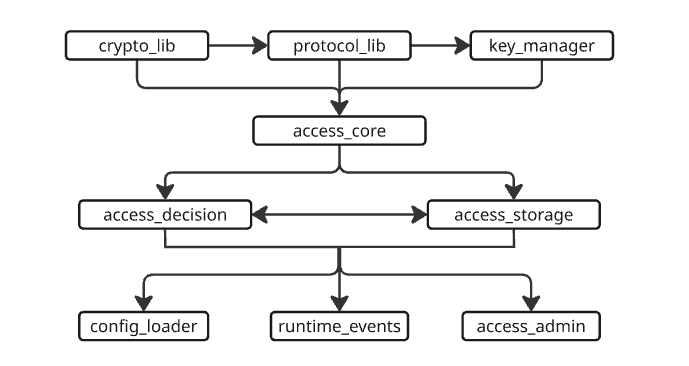
\includegraphics[width=0.72\textwidth]{plots/module_dependency.png}
\caption{Závislosťová hierarchia modulov projektu \texttt{access-security}
($A \rightarrow B$: modul $A$ závisí na $B$).}
\label{fig:module_deps}
\end{figure*}

\subsection{Externé závislosti}
\label{sec:third_party}

Prototyp využíva päť externých knižníc, ktoré sú zahrnuté v adresári \texttt{third\_party/} ako zdrojový kód kompilovaný spoločne s projektom. Takýto prístup (vendoring) zaručuje reprodukovateľnosť zostavenia --- projekt nie je závislý na systémových balíkoch, ktorých verzia a konfigurácia sa môže líšiť medzi prostrediami. Tabuľka~\ref{tab:third_party} uvádza zoznam závislostí s verziou a účelom.

\begin{table}[htbp]
\renewcommand{\arraystretch}{1.3}
\centering
\caption{Externé závislosti projektu}
\label{tab:third_party}
\small
\begin{tabular}{l l p{8.0cm}}
\toprule
\textbf{Knižnica} & \textbf{Verzia} & \textbf{Účel v projekte} \\
\midrule
libsodium\cite{LibsodiumDoc} & 1.0.20 & Kryptografické operácie: AEAD šifrovanie (ChaCha20-Poly1305, XChaCha20-Poly1305), HMAC-SHA-256, HKDF derivácia kľúčov, generovanie náhodných čísel, konštantné porovnávanie. \\
cpp-httplib\cite{CppHttplib} & 0.30.1 & Jednoduchý HTTP server a klient (header-only). Slúži ako základ REST API a administrátorského webového rozhrania. \\
nlohmann/json\cite{NlohmannJson} & 3.11.3 & Parsovanie a serializácia JSON správ medzi čítačkou, serverom a webovým rozhraním. \\
yaml-cpp\cite{YamlCpp} & 0.9.0 & Načítanie konfiguračného súboru \texttt{access\_security.yaml} s nastaveniami profilov, portov a databázy. \\
Google Test\cite{GoogleTest} & 1.14.0 & Unit a integračné testy. Používa sa pri verifikácii kvality kódu (44 testovacích prípadov). \\
\bottomrule
\end{tabular}
\end{table}

\noindent Z bezpečnostného hľadiska je najkritickejšou závislosťou knižnica \textbf{libsodium}, pretože na nej stojí celá kryptografická vrstva systému --- a teda aj všetky experimentálne výsledky tejto práce. Nasledujúca sekcia preto podrobne zdôvodňuje, prečo je analýza postavená na tejto knižnici validná.

\subsection{Zdôvodnenie použitia knižnice libsodium}
\label{sec:libsodium_justification}

Všetky kryptografické operácie v prototypovom systéme --- AEAD šifrovanie, HMAC autentifikácia, derivácia kľúčov, generovanie nonce, porovnávanie tagov --- sa vykonávajú prostredníctvom knižnice libsodium\cite{LibsodiumDoc}. Keďže experimentálna analýza v kapitole~\ref{sec:experiments} meria vlastnosti týchto operácií (odolnosť voči manipulácii, replay, cross-reader izoláciu, výkonnosť), je potrebné zdôvodniť, prečo sú výsledky získané cez libsodium relevantné nielen pre konkrétnu implementáciu, ale aj pre hodnotenie podkladových kryptografických konštrukcií.

\subsubsection{Súlad so štandardmi}

Libsodium implementuje algoritmy presne podľa príslušných štandardov:

\begin{itemize}[leftmargin=*,itemsep=2pt]
  \item \textbf{ChaCha20-Poly1305} (funkcia \texttt{crypto\_aead\_chacha20poly1305\_ietf}): implementácia podľa RFC~8439\cite{RFC8439}, vrátane IETF variantu s 96-bitovým nonce a 32-bitovým počítadlom blokov.
  \item \textbf{XChaCha20-Poly1305} (funkcia \texttt{crypto\_aead\_xchacha20poly1305}): konštrukcia podľa Internet-Draft\cite{XChaChaDraft}, kde sa 192-bitový nonce redukuje cez medzikrok HChaCha20\cite{Bernstein2012} na 96-bitový vstup pre ChaCha20.
  \item \textbf{HMAC-SHA-256} (funkcia \texttt{crypto\_auth\_hmacsha256}): podľa RFC~2104\cite{RFC2104} a FIPS~198-1\cite{FIPS1981}.
  \item \textbf{HKDF} (funkcie \texttt{crypto\_kdf\_hkdf\_sha256\_extract/expand}): podľa RFC~5869\cite{RFC5869}, dvojfázová derivácia (extract + expand) s SHA-256 ako podkladovou hash funkciou.
\end{itemize}

\noindent Súlad so štandardmi znamená, že vlastnosti analyzované v akademickej literatúre (napríklad odolnosť AEAD konštrukcie voči nonce misuse za predpokladu unikátnych nonce\cite{RogawayNonceMisuse2004}, alebo bezpečnosť HKDF pri dostatočnej entropii vstupného materiálu\cite{RFC5869}) sa prenášajú na našu implementáciu za predpokladu, že samotná knižnica neobsahuje chyby.

\subsubsection{Bezpečnostné audity a nasadenie}

Libsodium bola podrobená nezávislému bezpečnostnému auditu (Private Internet Access / NCC~Group, 2017\cite{LibsodiumAudit}), ktorý nezistil kritické zraniteľnosti v kryptografických primitívach. Knižnica je súčasťou produkčných systémov s vysokými bezpečnostnými požiadavkami:

\begin{itemize}[leftmargin=*,itemsep=2pt]
  \item \textbf{WireGuard}\cite{WireGuard} --- VPN protokol integrovaný do jadra Linux od verzie 5.6, používa ChaCha20-Poly1305 ako primárny šifrovací algoritmus.
  \item \textbf{Signal Protocol} --- end-to-end šifrovanie v aplikáciách Signal, WhatsApp a iných; využíva Curve25519 a ChaCha20-Poly1305 z libsodium/NaCl.
  \item \textbf{Minisign, age, Keybase} --- nástroje na podpisovanie a šifrovanie s milónmi používateľov.
\end{itemize}

\noindent Široké nasadenie v bezpečnostne kritických aplikáciách poskytuje empirickú evidenciu, že implementácia je robustná a neobsahuje systematické chyby, ktoré by znehodnocovali výsledky postavené na nej.

\subsubsection{Ochrana proti bočným kanálom}

Pre experimentálnu analýzu je dôležité, že libsodium implementuje \emph{konštantné} (constant-time) operácie pre všetky kryptografické primitíva. Porovnávanie tagov prebieha cez \texttt{sodium\_memcmp()}, ktorý je garantovane nezávislý od obsahu vstupov. AEAD operácie neobsahujú dátovo závislé vetvenia ani prístupy do pamäte závislé od tajných kľúčov\cite{LibsodiumDoc}. To znamená, že namerané časy v scenári S6 (throughput) odrážajú skutočnú výpočtovú náročnosť algoritmov, nie artefakty timing leakov.

\subsubsection{Kompilácia zo zdrojového kódu}

V projekte sa libsodium 1.0.20 kompiluje priamo zo zdrojového kódu pomocou CMake, nie ako predkompilovaný binárny balík. Tým je zaručené:

\begin{enumerate}[leftmargin=*,itemsep=2pt]
  \item \textbf{Známa a fixovaná verzia} --- experimenty sú reprodukovateľné s identickým kódom knižnice.
  \item \textbf{Rovnaké optimalizácie pre oba algoritmy} --- kompilátor (GCC/Clang) aplikuje rovnaké optimalizačné flagy (\texttt{-O2}) na zdrojové súbory oboch AEAD variantov. Zdrojový kód libsodium navyše obsahuje runtime detekciu SIMD inštrukčných sád (AVX2, SSSE3) a automaticky vyberá najrýchlejšiu implementáciu pre danú platformu\cite{LibsodiumDoc}.
  \item \textbf{Absencia externých patchov} --- zdrojový kód je identický s oficiálnym vydaním, čo vylučuje možnosť, že namerané výsledky sú ovplyvnené modifikáciou knižnice.
\end{enumerate}

\subsubsection{Záver k validite analýzy}

Na základe vyššie uvedených argumentov možno konštatovať, že výsledky experimentov v tejto práci:
\begin{itemize}[leftmargin=*,itemsep=2pt]
  \item sú \textbf{relevantné pre hodnotenie kryptografických konštrukcií} (ChaCha20-Poly1305, XChaCha20-Poly1305, HMAC-SHA-256, HKDF), pretože libsodium ich implementuje v súlade so štandardmi a bez známych odchýlok,
  \item sú \textbf{relevantné pre hodnotenie architektonických mechanizmov} (anti-replay, anomálna detekcia, karanténa, AAD binding), pretože tieto mechanizmy sú implementované v projektovom kóde a libsodium v nich pôsobí len ako korektná čierna skrinka,
  \item \textbf{nie sú automaticky prenositeľné} na iné implementácie tých istých algoritmov --- konkrétne namerané priepustnosti a latencie sú vlastnosťou libsodium 1.0.20 na danej platforme, nie abstraktnou vlastnosťou algoritmov (túto otázku podrobnejšie rozoberáme v kapitole~\ref{sec:experiments}, Tézis~6).
\end{itemize}

% TODO: Obrázok 6 --- Sekvenčný diagram protokolu: tri lifelines (ESP32, Server/hw\_service, DecisionEngine), postupnosť správ: POST /api/hw/uid → overenie HMAC podpisu → konštrukcia frame → handleFrameBytes → FrameHandler (replay, AEAD) → AnomalyDetector → RBAC → DecisionResult → HTTP odpoveď.

\subsection{Tok spracovania prístupovej udalosti}

Z pohľadu celého systému je najdôležitejší tok jednej prístupovej udalosti. V implementácii má tento tok niekoľko jasne oddelených krokov:

\begin{enumerate}[leftmargin=*,itemsep=3pt]
  \item Čítačka ESP32 načíta UID karty a prevedie ho na textový hexadecimálny tvar.
  \item Firmware pripojí \texttt{reader\_id}, \texttt{door\_id} a monotónny čítač \texttt{hw\_seq}, ktorý je uložený v \texttt{Preferences}, aby prežil reštart zariadenia.
  \item Zo surového JSON tela sa vytvorí podpis HMAC-SHA256 a požiadavka sa odošle na endpoint \texttt{/api/hw/uid}.
  \item Server v module \texttt{access\_admin} overí podpis \texttt{X-HW-Signature}. Ak podpis nesedí, požiadavka je zamietnutá ešte pred spracovaním biznis logiky.
  \item Po úspešnom overení sa požiadavka prevedie na interný payload \texttt{\{"card\_id": ..., "action": "open"\}} a pomocou \texttt{KeyManager} sa získa AEAD kľúč podľa \texttt{reader\_id} a aktuálnej verzie kľúča.
  \item Server vytvorí interný frame: zostaví hlavičku \texttt{reader\_id}, \texttt{door\_id}, \texttt{ts\_unix\_ms}, \texttt{seq}, \texttt{key\_version} a \texttt{nonce}; payload následne zašifruje konfigurovateľným AEAD algoritmom (ChaCha20-Poly1305 alebo XChaCha20-Poly1305 podľa aktívneho profilu).
  \item \texttt{DecisionEngine} odovzdá frame do \texttt{FrameHandler}, ktorý vykoná parsovanie, kontrolu väzby reader--door, kontrolu verzie kľúča, anti-replay kontrolu a dešifrovanie payloadu.
  \item Po úspešnom dešifrovaní sa payload interpretuje ako žiadosť o otvorenie dverí. Server dopočíta HMAC identifikátora karty, nájde zodpovedajúcu rolu a overí, či má táto rola oprávnenie pre konkrétne dvere.
  \item Výsledok sa uloží do auditnej stopy, odošle sa do \texttt{runtime\_events} a v jednoduchej JSON podobe sa vráti späť zariadeniu.
\end{enumerate}

Dôležitý je najmä krok medzi prijatím HTTP požiadavky a volaním \texttt{DecisionEngine}. V tejto implementácii zariadenie neposiela hotový šifrovaný frame priamo po sieti. Namiesto toho posiela autentifikovanú požiadavku s UID a \texttt{hw\_seq}; až server z nej vytvorí interný frame, ktorý ďalej spracúva rovnakou cestou ako zvyšok jadra. Z hľadiska práce je to dôležité, pretože sa tým jasne oddeľuje ochrana vstupu zariadenia (HMAC + sekvencia) od ochrany interného spracovania (AEAD + kontrola frame + audit).

\subsection{Poznámka k implementačným rozhodnutiam a k ďalšiemu spracovaniu textu}

Pri podrobnejšom čítaní kódu sa ukazuje, že nie všetky bezpečnostné mechanizmy sú koncentrované na jednom mieste. Napríklad anti-replay nie je iba vlastnosťou hardvéru, ale vzniká kombináciou \texttt{hw\_seq} vo firmvéri, serverovej validácie HMAC požiadavky a následnej kontroly v \texttt{ReplayWindow}. Podobne audit nie je len databázová tabuľka, ale súčasť rozhodovacieho toku, pretože \texttt{DecisionEngine} zapisuje auditné udalosti priamo pri spracovaní výsledku.

Z tohto dôvodu v ďalšom texte rozoberám praktickú časť podľa mechanizmov: autentifikácia hardvérového zariadenia, interné AEAD spracovanie, derivácia kľúčov, anti-replay, ochrana identifikátorov a auditná integrita. Takto rozdelený opis implementácie vytvára pevnú oporu pre neskoršie testy odolnosti, výkonnosti a detekcie manipulácie.

\subsection{Autentifikácia hardvérovej požiadavky}

Prvý kontrolný bod v celom toku spracovania je overenie, či HTTP požiadavka skutočne pochádza z registrovaného zariadenia. Zariadenie posiela na server JSON telo s poľami \texttt{uid}, \texttt{reader\_id}, \texttt{door\_id} a \texttt{hw\_seq}. Ako vstup do HMAC-SHA-256 slúži kanonický reťazec zložený z metódy, cesty a surového tela požiadavky:

\begin{equation}
\texttt{msg} = \texttt{\char34 POST /api/hw/uid\textbackslash n\char34} \parallel \texttt{raw\_body}
\end{equation}

Výsledný podpis sa prenáša v HTTP hlavičke \texttt{X-HW-Signature} ako hexadecimálny reťazec. Na strane servera sa HMAC prepočíta nad rovnakým kanonickým vstupom a porovná s hodnotou z hlavičky. Porovnanie prebieha konštantným časom cez funkciu \texttt{sodium\_memcmp} z knižnice libsodium, čo výrazne znižuje riziko timing útoku, pri ktorom by útočník mohol postupne odhadovať správny podpis podľa dĺžky odpovede\cite{FIPS1981,RFC2104}.

Kanonizácia je v tomto prípade dôležitý detail. Zariadenie aj server musia pracovať s identickým blokom bajtov, pretože aj jediný rozdiel v poradí polí, whitespace alebo kódovaní spôsobí nesúlad podpisu. V prototypovej implementácii je to riešené tak, že sa podpisuje surové telo požiadavky (\emph{raw body}), nie jeho štruktúrovaná JSON reprezentácia. Zariadenie vždy generuje JSON s pevne definovaným poradím polí, takže riziko nesúladu je minimálne.

Táto konštrukcia zabezpečuje dve vlastnosti. Overuje pôvod požiadavky: útočník, ktorý nedisponuje zdieľaným tajomstvom, nevie vyrobiť platný podpis. A overuje integritu obsahu: zmena ľubovoľného poľa v JSON tele (napríklad podvrhnutie iného \texttt{uid} alebo \texttt{door\_id}) spôsobí zlyhanie verifikácie.

Zariadenie pri tom nepoužíva administrátorský token \texttt{X-Admin-Token}, ktorý je určený výhradne pre správcovské rozhranie. Oddelenie kanálov autentifikácie vychádza z princípu najmenších oprávnení: aj keby útočník kompromitoval čítačku a získal jej HMAC tajomstvo, nezískal by tým prístup na zmenu rolí, kariet ani väzieb medzi čítačkou a dverami\cite{OWASPAPI2023}.

\subsection{AEAD šifrovanie interného frame}

Po úspešnom overení hardvérovej požiadavky server nevyhodnocuje prístup priamo z prijatých dát. Namiesto toho z nich vytvára interný bezpečný frame: binárnu štruktúru, v ktorej je payload zašifrovaný algoritmom AEAD a hlavička je kryptograficky previazaná cez mechanizmus Associated Authenticated Data.

\subsubsection{Voľba algoritmu}

V implementácii sa používajú dva AEAD algoritmy z rodiny ChaCha20-Poly1305, oba postavené na rovnakom kryptografickom jadre (ChaCha20 stream cipher + Poly1305 MAC) a oba so 256-bitovou kľúčovou bezpečnosťou:

\begin{itemize}[leftmargin=*,itemsep=2pt]
  \item \textbf{XChaCha20-Poly1305} s 192-bitovým noncom (24 bajtov). Rozšírený nonce je konštruovaný pomocou medzikroku HChaCha20, vďaka čomu je bezpečné používať náhodne generované nonce aj pod dlhodobo žijúcim kľúčom: pravdepodobnosť kolízie pri $2^{96}$ správach je zanedbateľná\cite{XChaChaDraft,LibsodiumXChaChaDoc}.
  \item \textbf{ChaCha20-Poly1305 IETF} s 96-bitovým noncom (12 bajtov). Štandardizovaný v RFC 8439 a široko nasadzovaný v TLS 1.3 aj v ďalších protokoloch\cite{RFC8439}. Kratší nonce znižuje bezpečný limit pre náhodne generované nonce na približne $2^{48}$ správ.
\end{itemize}

Implementácia podporuje tri stratégie generovania nonce, označené R0, R1 a R2 (podrobnejšie v nasledujúcej podsekcii). Pri deterministickej konštrukcii (R1, R2) je riziko kolízie pre oba algoritmy identické: nonce sa zopakuje iba vtedy, keď sa zopakuje vstupný kontext, čomu bráni kombinácia anti-replay mechanizmu a unikátneho \texttt{seq}. Oba algoritmy sú preto zahrnuté v implementácii nie kvôli rozdielnej bezpečnosti, ale kvôli možnosti porovnať ich výkon a režijné náklady v experimentálnych profiloch.

Kryptografické operácie sú realizované výhradne cez knižnicu libsodium, konkrétne cez funkcie \texttt{crypto\_aead\_xchacha20poly1305\_ietf\_*} a \texttt{crypto\_aead\_chacha20poly1305\_ietf\_*}. Oba algoritmy vychádzajú z rodiny stream cipher primitív navrhnutých D.~J.~Bernsteinom\cite{Bernstein2012}. Rozhodnutie neimplementovať cipher suites vlastnou cestou je zámerné: libsodium je auditovaná knižnica s konštantnočasovou implementáciou, čo znižuje riziko implementačných chýb tejto triedy\cite{LibsodiumXChaChaDoc}.

\subsubsection{Konštrukcia nonce}

Implementácia definuje rozhranie \texttt{INonceGenerator} s jednou metódou \texttt{generate(context, seq)}, za ktorým stoja tri konkrétne stratégie:

\paragraph{R0: Náhodný nonce.}
Trieda \texttt{RandomNonceGenerator} ignoruje kontext aj sekvenčné číslo a pri každom volaní vygeneruje kryptograficky bezpečný náhodný nonce pomocou \texttt{randombytes\_buf}:

\begin{equation}
\text{nonce}_{\text{R0}} = \texttt{randombytes\_buf}(n) \qquad n \in \{12, 24\}
\end{equation}

Bezpečnosť tejto stratégie závisí na kvalite generátora náhodných čísiel a na počte správ pod jedným kľúčom. Pre XChaCha20 s 24-bajtovým noncom je riziko kolízie zanedbateľné do $2^{96}$ správ; pre ChaCha20 s 12-bajtovým noncom klesá bezpečná hranica na približne $2^{48}$.

\paragraph{R1/R2: Deterministický HMAC nonce.}
Trieda \texttt{HmacNonceGenerator} odvodzuje nonce deterministicky z dedikovaného kľúča $K_{\text{nonce}}$ a kontextu hlavičky frame. Kľúč sa odvodzuje cez HKDF-SHA-256 z master kľúča:

\begin{equation}
K_{\text{nonce}} = \text{HKDF-SHA-256}(K_{\text{master}},\; \texttt{reader\_id} \parallel \texttt{key\_version},\; \text{\texttt{\char34 nonce-derivation-v1\char34}})
\end{equation}

Samotný nonce sa počíta ako skrátený výstup HMAC-SHA-256 nad serializovanou hlavičkou (52~bajtov), v~ktorej je pole nonce vynulované, aby sa predišlo kruhovej závislosti:

\begin{equation}
\text{nonce}_{\text{R1/R2}} = \text{HMAC-SHA-256}(K_{\text{nonce}},\; \texttt{header\_context})\;[:n] \qquad n \in \{12, 24\}
\end{equation}

kde $\texttt{header\_context} = \texttt{reader\_id} \parallel \texttt{door\_id} \parallel \texttt{ts\_unix\_ms} \parallel \texttt{seq} \parallel \texttt{key\_version} \parallel 0^{24}$ v~little-endian formáte.

Deterministická konštrukcia znižuje závislosť na kvalite generátora náhodných čísiel\cite{BellareNonceMisuse2006}. Nonce sa zopakuje iba vtedy, keď sa zopakuje celý kontext, čomu bráni unikátnosť \texttt{seq} garantovaná anti-replay mechanizmom. Navyše, keďže kontext obsahuje aj \texttt{door\_id} a \texttt{ts\_unix\_ms}, rovnaký nonce nevznikne ani pri rôznych kontextoch s rovnakým sekvenčným číslom.

\paragraph{Rozdiel medzi R1 a R2.}
Stratégie R1 a R2 používajú identický \texttt{HmacNonceGenerator}. Odlišuje ich to, či server po vytvorení frame \emph{overuje}, že prijatý nonce zodpovedá deterministickému výpočtu. Overenie vykonáva \texttt{ProtocolAnomalyDetector} (sekcia~\ref{sec:anomaly_detector}), ktorý je aktívny iba v~profiloch R2. V~profiloch R1 je detektor vypnutý: nonce sa síce generuje deterministicky, ale server akceptuje frame bez verifikácie nonce zhody.

Na drôtovom formáte frame zaberá pole nonce vždy 24 bajtov kvôli uniformnej štruktúre hlavičky. Pri profile A2 (XChaCha20-Poly1305) sa využíva celých 24 bajtov; pri profile A1 (ChaCha20-Poly1305) sa používa prvých 12 bajtov a zvyšných 12 je nulových. Táto konvencia zjednodušuje parsovanie a zaručuje, že veľkosť hlavičky je rovnaká naprieč všetkými profilmi.

\subsubsection{AAD väzba hlavičky}

Hlavička frame obsahuje polia \texttt{reader\_id}, \texttt{door\_id}, \texttt{ts\_unix\_ms}, \texttt{seq}, \texttt{key\_version} a \texttt{nonce}. Tieto metadáta sa nešifrujú, ale vstupujú do AEAD operácie ako AAD. Výsledkom je, že zmena ktoréhokoľvek z nich spôsobí zlyhanie overenia autentifikačného tagu, aj keď šifrovaný payload zostane neporušený\cite{RFC5116}.

Praktický význam tejto väzby sa ukáže pri konkrétnom útoku. Bez AAD by útočník mohol zachytiť platný frame a podvrhnúť hodnotu \texttt{door\_id}: payload by bol stále korektne dešifrovaný, no systém by vyhodnotil prístup pre iné dvere. AAD toto znemožňuje, pretože kryptograficky viaže šifrovaný obsah na presný kontext metadát. Ide o realizáciu princípu, že kontext autorizácie musí byť nedeliteľnou súčasťou správy.

Implementácia podporuje aj konfigurovateľný režim \texttt{aad\_mode: "none"}, v~ktorom sa AAD nepoužíva a hlavička nie je kryptograficky chránená. Tento režim je v~kóde prítomný ako záložná možnosť, no \emph{nie je súčasťou experimentálnej matice}: všetkých šesť testovaných profilov (A1-R0 až A2-R2) používa plnú AAD väzbu (\texttt{aad\_mode: "full"}). Dopad absencie AAD sa demonštruje nepriamo --- scenárom S2 (field tampering), kde útočník mení \texttt{door\_id} v~hlavičke a~AAD väzba spôsobí zlyhanie autentifikačného tagu.

\subsection{Derivácia kľúčov a domain separation}

Celý kryptografický materiál v prototype pochádza z jedného 256-bitového master secret, uloženého v súbore \texttt{secrets/master\_key.hex} mimo repozitára. Manuálne spravovaný tajný súbor je pragmatický kompromis vhodný pre prototyp; v produkčnom nasadení by jeho úlohu plnil HSM alebo vault\cite{NIST80057}. Z tohto tajomstva sa pomocou HKDF-SHA-256\cite{RFC5869} deterministicky odvodia tri nezávislé skupiny podkľúčov:

\begin{enumerate}[leftmargin=*,itemsep=2pt]
  \item \textbf{AEAD kľúče} pre šifrovanie interného frame. Salt je zložený z \texttt{reader\_id} (4 bajty, little-endian) a \texttt{key\_version} (4 bajty), info reťazec je \texttt{"access-aead-v1"}.
  \item \textbf{Nonce kľúče} pre deterministickú deriváciu nonce (stratégie R1/R2). Salt je rovnaký ako pri AEAD kľúčoch (\texttt{reader\_id} $\parallel$ \texttt{key\_version}), info reťazec je \texttt{"nonce-derivation-v1"}.
  \item \textbf{Pepper} pre hashovanie identifikátorov kariet. Salt obsahuje iba \texttt{key\_version}, info reťazec je \texttt{"card-pepper-v1"}.
  \item \textbf{Auditný HMAC kľúč} pre hash chain. Salt je \texttt{"audit-chain-salt-v1"}, info reťazec \texttt{"audit-hmac-v1"}.
\end{enumerate}

\begin{table}[htbp]
\renewcommand{\arraystretch}{1.3}
\centering
\caption{Prehľad HKDF derivácie kľúčov z master secret}
\label{tab:hkdf-keys}
\small
\begin{tabular}{l l l}
\toprule
\textbf{Kľúč} & \textbf{Salt} & \textbf{Info reťazec} \\
\midrule
AEAD & \texttt{reader\_id} $\parallel$ \texttt{key\_ver} & \texttt{access-aead-v1} \\
Nonce ($K_{\text{nonce}}$) & \texttt{reader\_id} $\parallel$ \texttt{key\_ver} & \texttt{nonce-derivation-v1} \\
Pepper & \texttt{key\_ver} & \texttt{card-pepper-v1} \\
Auditný HMAC & \texttt{audit-chain-salt-v1} & \texttt{audit-hmac-v1} \\
\bottomrule
\end{tabular}
\end{table}

Grafické znázornenie tejto derivačnej hierarchie je v obrázku~\ref{fig:hkdf_tree}.

\begin{figure*}[htbp]
\centering
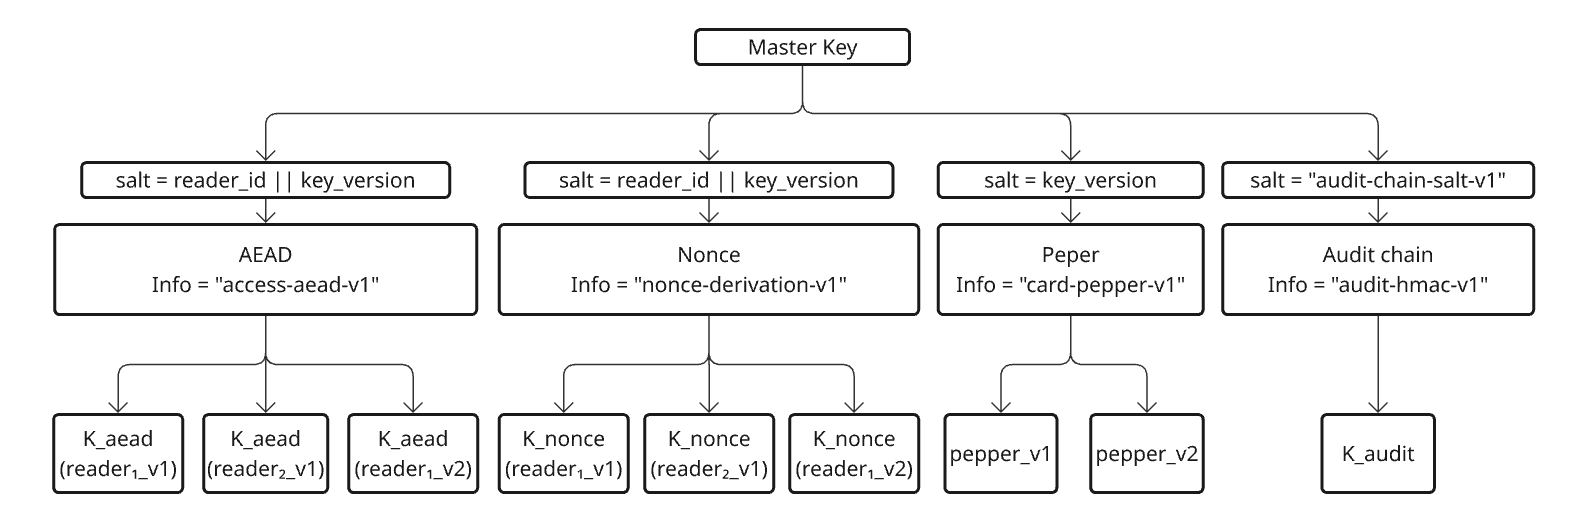
\includegraphics[width=0.92\textwidth]{plots/hkdf_derivation_tree.png}
\caption{Derivácia kľúčov z master secret cez HKDF. Každá vetva má vlastný \texttt{info} reťazec (domain separation).}
\label{fig:hkdf_tree}
\end{figure*}

Info reťazce zabezpečujú domain separation\cite{RFC5869}: z rovnakého master kľúča nikdy nevznikne rovnaký podkľúč pre dva rôzne účely, ani keby sa hodnoty \texttt{reader\_id} a \texttt{key\_version} náhodne prekrývali. Súčasne umožňujú neskoršiu zmenu verzie schémy (napríklad z \texttt{access-aead-v1} na \texttt{access-aead-v2}) bez spätnej kompatibility so starými kľúčmi, čo je dôležité pri migračných scenároch.

Z bezpečnostného hľadiska je podstatné, že AEAD kľúč sa odvodzuje per-reader. Kompromitácia jedného zariadenia a extrakcia jeho odvoditeľného kľúča neodhaľuje kľúče iných čítačiek, pretože salt HKDF obsahuje unikátnu hodnotu \texttt{reader\_id}. Izolácia je priamym dôsledkom správnej konštrukcie derivácie a nevyžaduje distribúciu samostatných tajomstiev.

Verzovanie kľúčov v salt zabezpečuje, že pri rotácii (zmene \texttt{key\_version}) sa odvodí úplne nový AEAD kľúč bez nutnosti meniť master secret. Server v konfigurácii umožňuje režim \texttt{allow\_previous\_key\_version}, v ktorom dočasne akceptuje aj bezprostredne predchádzajúcu verziu. Cieľom je hladký prechod pri rotácii: zariadenie nemusí byť aktualizované presne v rovnakom okamihu ako server, čo znižuje riziko krátkodobého výpadku\cite{NIST80057}.

Implementácia podporuje aj režim \texttt{key\_derivation\_mode: "direct"}, v~ktorom sa HKDF nepoužíva a master kľúč slúži priamo ako AEAD kľúč pre všetky čítačky. Podobne ako pri \texttt{aad\_mode}, tento režim je v~kóde prítomný ako záložná možnosť, ale \emph{nie je súčasťou experimentálnej matice}. Všetky profily používajú HKDF deriváciu s~per-reader salt, čím je zaručená izolácia kľúčov medzi čítačkami. Experimenty sa zameriavajú na premenné s~priamejším dopadom na odolnosť voči útokom: voľbu AEAD algoritmu (A1/A2), stratégiu generovania nonce (R0/R1/R2) a~prítomnosť anomálneho detektora.

\subsection{Anti-replay mechanizmus}

Anti-replay ochrana funguje na dvoch úrovniach. Na strane zariadenia firmvér udržiava monotónne počítadlo \texttt{hw\_seq}, uložené v NVS pamäti ESP32, ktoré sa inkrementuje pri každom skene karty a prežíva reštart zariadenia. Každá požiadavka tak nesie unikátnu sekvenčnú hodnotu.

Na strane servera modul \texttt{protocol\_lib} implementuje štruktúru \texttt{ReplayWindow}, ktorá udržiava záznam o naposledy videných sekvenciách pre každú čítačku zvlášť. Mechanizmus rozlišuje tri stavy:

\begin{itemize}[leftmargin=*,itemsep=2pt]
  \item ak je \texttt{seq} menšie než \texttt{maxSeen $-$ windowSize}, požiadavka sa odmietne ako príliš stará,
  \item ak \texttt{seq} spadá do okna, ale už bolo zaznamenané, odmietne sa ako \emph{replay},
  \item inak sa \texttt{seq} akceptuje, zaznamená do množiny videných hodnôt a posunie sa horná hranica okna.
\end{itemize}

Prečo nestačí jednoduchá podmienka \texttt{seq > lastSeen}? V prostredí Wi-Fi nie je zaručené, že dve po sebe nasledujúce požiadavky dorazia na server v rovnakom poradí. Bez okna by druhá požiadavka bola nesprávne odmietnutá, aj keď by bola legitímna. Sliding window toleruje krátke zmeny poradia, pokiaľ správa ešte nebola videná, a tým znižuje podiel falošných odmietnutí pri zachovaní replay ochrany.

Veľkosť okna (\texttt{replay\_window\_size}) je konfigurovateľná a priamo ovplyvňuje kompromis medzi bezpečnosťou a praktickou použiteľnosťou: príliš malé okno zvyšuje falošné odmietnutia, príliš veľké predlžuje čas, počas ktorého je zachytená stará požiadavka potenciálne zopakovateľná. Implementácia udržiava okno pomocou fronty (\texttt{std::deque}) a množiny (\texttt{std::unordered\_set}), pričom pri prekročení kapacity sa najstaršia hodnota automaticky evikvuje.

% TODO: Obrázok 4 --- Sliding replay window vizualizácia: horizontálna číselná os (seq čísla), tri zóny farebne odlíšené (sivá = príliš staré, zelená = akceptované, červená = už videné), šípka maxSeen a posun okna pri novom seq.

\subsection{Detektor protokolových anomálií}
\label{sec:anomaly_detector}

Nad rámec reaktívneho odmietnutia jednotlivých frame implementácia obsahuje komponent \texttt{ProtocolAnomalyDetector}, ktorý sleduje vzory správania na úrovni celej čítačky a pri podozrivej aktivite dokáže čítačku proaktívne umiestniť do karantény. Tento prístup vychádza z princípov detekcie anomálií v sieťovom prostredí\cite{NIST80094}.

Detektor udržiava per-reader stavový záznam a~sleduje štyri typy anomálií:

\begin{enumerate}[leftmargin=*,itemsep=2pt]
  \item \textbf{Opakované sekvenčné číslo} (\texttt{seq\_reuse}): ak frame nesie \texttt{seq}, ktoré už bolo zaznamenané. Na rozdiel od \texttt{ReplayWindow}, ktorá frame iba odmietne, detektor túto udalosť zaregistruje ako indikátor replay útoku.
  \item \textbf{Rollback sekvenčného čísla} (\texttt{seq\_rollback}): ak \texttt{seq + rollbackThreshold < maxSeenSeq}. Veľký skok späť signalizuje, že útočník sa pokúša obísť sliding window opakovaním starších sekvencií.
  \item \textbf{Nesúlad nonce} (\texttt{nonce\_mismatch}): ak prijatý nonce nezodpovedá deterministicky odvodenému nonce z kontextu hlavičky. Táto kontrola je aktívna iba v~profiloch s~\texttt{nonceMode = "deterministic"} (R1/R2), no v~kóde je podmienená \emph{aj} zapnutím detektora --- preto sa vykonáva iba v~profiloch R2.
  \item \textbf{Séria zlyhaní tagu} (\texttt{tag\_fail\_streak}): ak počet po sebe nasledujúcich zlyhaní AEAD autentifikačného tagu dosiahne konfigurovateľný limit. Opakované zlyhania indikujú brute-force pokus o~uhádnutie platného ciphertextu.
\end{enumerate}

Pri detekcii anomálie sa čítačka umiestni do karantény: všetky ďalšie frame od tejto čítačky sú zamietnuté s~dôvodom \texttt{reader\_quarantined}, bez ohľadu na ich obsah. Karanténa je proaktívna obrana --- izoluje celé zariadenie, nie iba jednotlivý frame. Tým sa odlišuje od anti-replay okna (ktoré zamieta iba konkrétnu sekvenciu) a~od zlyhania AEAD dešifrovania (ktoré zamieta iba frame s~neplatným tagom).

V~experimentálnej matici je detektor zapnutý výhradne v~profiloch R2 (A1-R2, A2-R2). Profily R0 a R1 majú detektor vypnutý, čo umožňuje v~scenároch S1--S5 presne kvantifikovať jeho prínos: profily R0/R1 vykazujú nenulovú úspešnosť útoku (napr. 11\,\% v~S4), zatiaľ čo R2 dosahuje 0\,\% vďaka okamžitej karanténe po prvej anomálii.

\begin{table}[htbp]
\renewcommand{\arraystretch}{1.3}
\centering
\caption{Konfigurácia \texttt{ProtocolAnomalyDetector} a reakcia na anomálie}
\label{tab:anomaly-config}
\begin{tabular}{l l l}
\toprule
\textbf{Typ anomálie} & \textbf{Podmienka detekcie} & \textbf{Reakcia} \\
\midrule
\texttt{seq\_reuse} & $\texttt{seq} \in \texttt{\_seen}$ & Okamžitá karanténa \\
\texttt{seq\_rollback} & $\texttt{seq} + \delta < \texttt{maxSeenSeq}$ & Okamžitá karanténa \\
\texttt{nonce\_mismatch} & $\texttt{nonce} \neq \text{HMAC}(K_n, \text{ctx})[:n]$ & Okamžitá karanténa \\
\texttt{tag\_fail\_streak} & 5 po sebe nasledujúcich zlyhaní & Karanténa po 5. zlyhaní \\
\bottomrule
\end{tabular}
\end{table}

\subsection{Ochrana identifikátorov kariet}

Databáza neukladá surové UID kariet --- v súlade s princípom minimalizácie dát\cite{ISO27001} a ochranou identifikátorov\cite{NIST80063B4}. Pri registrácii aj pri vyhľadávaní sa UID prepočíta na HMAC hash s tajomstvom, ktoré v databáze uložené nie je:

\begin{equation}
\texttt{card\_hmac} = \mathrm{HMAC\text{-}SHA\text{-}256}(\texttt{pepper},\; \texttt{uid})
\end{equation}

Pri úniku databázy útočník získa iba výsledné HMAC hodnoty. Bez znalosti pepperu z nich nevie efektívne odvodiť pôvodné UID, a to ani pri relatívne malom priestore identifikátorov (napríklad 4-bajtové UID majú $2^{32}$ možností, čo by pri slabom hashovaní umožňovalo hrubú silu)\cite{FIPS1981}. Pepper sa odvodzuje cez HKDF z master kľúča a verzuje podľa \texttt{key\_version}. Pri rotácii pepperu sa musia existujúce karty prehashovať pod novým tajomstvom.

Rozdiel oproti klasickému salt-based hashov je zámerný. Salt sa ukladá vedľa hashu a jeho účelom je zabrániť predpočítaným tabuľkám (\emph{rainbow tables}); pepper sa naopak nachádza mimo úložiska a chráni aj proti slovníkovému útoku s priamym prístupom k databáze. Na druhej strane, ak útočník kompromituje server a získa pepper, ochrana sa stráca. Pepper preto nie je náhrada za kryptograficky silnú kartu, ale primeraná vrstva ochrany v rámci prototypu.

\subsection{Tamper-evident auditná stopa}

Auditný log v prototype nie je obyčajný záznam udalostí. Každý záznam obsahuje HMAC hash, ktorý kryptograficky viaže jeho obsah na celú predchádzajúcu históriu.

\subsubsection{Konštrukcia HMAC hash chain}

Základná konštrukcia vychádza z iteratívnej aplikácie HMAC na každý nový záznam:

\begin{equation}
H_i = \mathrm{HMAC}(K_{\text{audit}},\; H_{i-1} \parallel \mathrm{encode}(\text{record}_i))
\end{equation}

kde $K_{\text{audit}}$ je auditný kľúč odvodený cez HKDF z master secret a $H_{i-1}$ je hash predchádzajúceho záznamu. Pre prvý záznam sa používa $H_0 = 0^{32}$. Kanonikalizácia záznamu je deterministická

% TODO: Obrázok 5 --- Audit hash chain diagram: séria prepojených boxov (event₁, event₂, ..., anchor) s HMAC šípkami medzi nimi, znázornenie, že modifikácia event₂ zmení H₂ a všetky nasledujúce hodnoty, čím anchor nezodpovedá.: polia sa serializujú v pevne definovanom poradí (\texttt{ts\_unix\_ms}, \texttt{reader\_id}, \texttt{door\_id}, \texttt{seq}, \texttt{allow}, \texttt{reason}, \texttt{card\_hmac}, \texttt{action}) v little-endian formáte s explicitnými dĺžkami textových reťazcov\cite{SchneierKelsey1999}.

Reťazec hash hodnôt znamená, že zmena ľubovoľného záznamu spôsobí nekonzistenciu vo všetkých nasledujúcich hodnotách. Útočník, ktorý nemá auditný kľúč, nevie prepočítať $H_i$ od miesta zásahu tak, aby reťazec zostal konzistentný.

\subsubsection{Anchor a ochrana proti truncation}

Hash chain sám o sebe nezabráni útoku, pri ktorom útočník odstráni posledných $n$ záznamov a ponechá konzistentný prefix. Preto prototyp udržiava \emph{audit anchor}: po každom zápise sa aktuálna hodnota $H_i$ a timestamp uložia do samostatnej jednoriadkovej tabuľky \texttt{audit\_anchor}. Pri verifikácii sa kontroluje, že log obsahuje záznamy minimálne po poslednú hodnotu anchor. Ak záznamy chýbajú, ide o detekovateľný truncation\cite{SchneierKelsey1999,NIST80092}.

Anchor nie je úplná ochrana v prípade, že útočník má plný zápis do databázy --- v takom prípade vie prepísať aj anchor. Silnejšie riešenie by vyžadovalo uloženie anchor mimo databázy (napríklad na vzdialenom serveri alebo v hardvérovom module). V kontexte prototypu je cieľom demonštrovať princíp detekcie manipulácie, nie dosiahnuť odolnosť voči útočníkovi s neobmedzeným prístupom.

Implementácia navyše rozlišuje medzi reťazeným a nereťazeným režimom auditu. Ak je reťazenie vypnuté, záznamy sa ukladajú s nulovými hodnotami \texttt{prev\_hash} a \texttt{entry\_hash}, čo zodpovedá jednoduchému logu bez kryptografickej ochrany. Porovnanie oboch režimov v analytickej časti demonštruje presný dopad tejto ochrany.

\subsection{Rozhodovacia logika a model RBAC}

Na konci spracovateľského reťazca stojí \texttt{DecisionEngine}, ktorý po úspešnom dešifrovaní payloadu vyhodnocuje, či má byť prístup povolený. Rozhodovanie prebieha v niekoľkých krokoch. Server prepočíta HMAC identifikátora karty s aktuálnym pepperom. V tabuľke \texttt{cards} vyhľadá kartu podľa výsledného \texttt{card\_hmac}. Ak ju nájde, prečíta jej rolu; ak nie, výsledok je \texttt{deny} s dôvodom \texttt{unknown\_card}. Nakoniec v tabuľke \texttt{door\_roles} overí, či rola karty je povolená pre dvere z hlavičky frame\cite{NISTRBACModel,SandhuRBAC1996}.

Model RBAC v prototype znamená, že karty nemajú priame oprávnenia na dvere. Sú im priradené roly (napríklad \emph{employee}, \emph{admin}) a dvere majú povolené zoznamy rolí. Pridanie alebo odobratie oprávnenia sa robí na úrovni väzby rola--dvere, nie na úrovni jednotlivých kariet. To zjednodušuje správu pri veľkom počte používateľov a umožňuje rýchlu revokáciu: zrušenie roly v tabuľke \texttt{door\_roles} okamžite odmietne všetky karty s touto rolou pre dané dvere.

Výsledok rozhodnutia (\texttt{allow} alebo \texttt{deny}) sa spolu s identifikátorom čítačky, dverí, sekvenčným číslom a dôvodom zapíše do tamper-evident auditnej stopy. Dôvod zamietnutia (\texttt{reason}) je interný diagnostický kód (napríklad \texttt{replay}, \texttt{unknown\_card}, \texttt{mac\_verification\_failed}), ktorý sa nezverejňuje nedôveryhodnému klientovi, ale ukladá sa do auditu a zobrazuje v administrátorskom rozhraní. Tým sa zabezpečuje, že diagnostika je k dispozícii prevádzke, no útočník z odpovede nezíska informácie užitočné pre iteráciu útoku.

\subsection{Konfigurácia systému a bezpečnostné profily}

Správanie bezpečnostných mechanizmov prototypu je plne konfigurovateľné cez súbor \texttt{config/access\_security.yaml}, ktorý server načítava pri štarte. Konfigurácia rozlišuje tri úrovne parametrov:

\begin{description}[leftmargin=*,itemsep=2pt]
  \item[Serverové parametre:] hostiteľ, port, maximálna veľkosť payloadu, cesta k databáze, maximálna prípustná časová odchýlka (\texttt{max\_skew\_ms}).
  \item[Kryptografické parametre:] voľba AEAD algoritmu (\texttt{cipher\_mode}: \texttt{xchacha20poly1305} alebo \texttt{chacha20poly1305}), režim generovania nonce (\texttt{nonce\_mode}: \texttt{random} / \texttt{deterministic}), režim AAD (\texttt{aad\_mode}: \texttt{full} / \texttt{none"}), režim derivácie kľúčov (\texttt{key\_derivation\_mode}: \texttt{hkdf} / \texttt{direct}).
  \item[Prevádzkové parametre:] veľkosť replay window (\texttt{replay\_window\_size}, predvolene 256), povolenie predchádzajúcej verzie kľúča (\texttt{allow\_previous\_key\_version}), stav detektora anomálií (\texttt{anomaly\_detector\_enabled}), prahy detektora (\texttt{rollback\_threshold}: 100, \texttt{tag\_fail\_streak\_limit}: 5).
\end{description}

\begin{table}[htbp]
\renewcommand{\arraystretch}{1.3}
\centering
\caption{Kľúčové konfiguračné parametre a ich mapovanie na bezpečnostné profily}
\label{tab:config-params}
\small
\begin{tabular}{l l l}
\toprule
\textbf{Parameter} & \textbf{Hodnoty} & \textbf{Experimentálne profily} \\
\midrule
\texttt{cipher\_mode} & \texttt{chacha20poly1305} & A1 \\
 & \texttt{xchacha20poly1305} & A2 \\
\texttt{nonce\_mode} & \texttt{random} & R0 \\
 & \texttt{deterministic} & R1, R2 \\
\texttt{anomaly\_detector\_enabled} & \texttt{false} & R0, R1 \\
 & \texttt{true} & R2 \\
\texttt{aad\_mode} & \texttt{full} & všetky 6 profilov \\
\texttt{key\_derivation\_mode} & \texttt{hkdf} & všetky 6 profilov \\
\texttt{replay\_window\_size} & 256 & všetky 6 profilov \\
\bottomrule
\end{tabular}
\end{table}

\noindent Toto oddelenie konfigurácie od kódu umožňuje prepínať profily bez rekompilácie a zaručuje, že experimentálny harness aj produkčný server môžu využívať rovnakú implementačnú logiku --- menia sa iba parametre, nie kód. Konfigurácia zároveň obsahuje explicitné záložné hodnoty (\texttt{aad\_mode: none} a \texttt{key\_derivation\_mode: direct}), ktoré slúžia pre diagnostiku a ladenie, ale nie sú súčasťou experimentálnej matice.

\subsection{Webové administrátorské rozhranie}

Modul \texttt{access\_admin} okrem REST API servíruje aj webové rozhranie dostupné na \texttt{/static/}. Rozhranie je implementované v čistom JavaScripte bez externého frameworku a sprostredkúva priamy prístup ku všetkým správcovským operáciám:

\begin{itemize}[leftmargin=*,itemsep=2pt]
  \item \textbf{Správa čítačiek, dverí, rolí a kariet:} CRUD operácie nad databázovými entitami; karty sa registrujú zadaním UID, ktoré server okamžite prepočíta na HMAC hash pred uložením.
  \item \textbf{Väzby reader--door:} priradenie čítačky ku konkrétnym dverám; táto väzba je vynucovaná aj na úrovni kryptografickej AAD hlavičky.
  \item \textbf{Live log:} real-time stream posledných 50 rozhodnutí cez polling endpointu \texttt{/api/events}; zobrazuje profil, výsledok, dôvod zamietnutia a latenciu.
  \item \textbf{Auditná verifikácia:} tlačidlo na spustenie offline verifikácie integrity hash chain; výsledok zobrazuje počet záznamov, stav reťaze a prípadnú polohu prvej nekonzistencie.
  \item \textbf{Import/export databázy:} JSON export aktuálneho stavu, JSON import pre migráciu konfigurácie.
\end{itemize}

Autentifikácia administrátorského rozhrania je realizovaná hlavičkou \texttt{X-Admin-Token}, ktorá je striktne oddelená od HMAC autentifikácie zariadení (princíp najmenej oprávnení\cite{SaltzerSchroeder1975}): kompromitácia čítačky nedáva útočníkovi prístup k správcovskej funkcionalite a naopak.

\subsection{Prepojenie mechanizmov: prečo vrstvy nestoja samostatne}

Popísané mechanizmy nie sú navzájom nezávislé bezpečnostné funkcie, ale navrhnuté tak, aby sa dopĺňali v zmysle princípu defense-in-depth\cite{DefenseInDepth,NIST80053}. HMAC autentifikácia zariadenia by bola neúčinná bez anti-replay, pretože by stačilo zachytiť jednu platnú požiadavku a opakovať ju. Anti-replay bez HMAC by bol zbytočný, pretože útočník by mohol vyrobiť ľubovoľnú novú požiadavku s nepoužitým \texttt{seq}. AEAD bez AAD by chránilo dôvernosť payloadu, ale nie kontext autorizácie. A audit bez hash chain by bol dôveryhodný iba do momentu, kým by sa útočník nedostal k databáze.

Práve toto vzájomné prepojenie je jedným z hlavných predmetov analytickej časti. Experimentálna matica šiestich profilov (A1-R0 až A2-R2) variuje AEAD algoritmus, stratégiu generovania nonce a~prítomnosť anomálneho detektora, pričom ostatné vrstvy (AAD väzba, HKDF derivácia, pepper, anti-replay okno) zostávajú vo všetkých profiloch zapnuté. Šesť scenárov (S1--S6) potom ukazuje, ktorá konkrétna kombinácia vrstiev chráni proti ktorému konkrétnemu útoku --- a~naopak, kde samotná zmena jednej premennej (napríklad prechod z~R1 na R2) dokáže eliminovať celú triedu útokov.

\section{Verifikácia kvality kódu pred experimentmi}

Pred vykonaním akýchkoľvek experimentov je nutné overiť, že implementácia samotná neobsahuje chyby pamäťového prístupu, nedefinované správanie, pretečenia bufferov či úniky pamäte. Ak by takéto defekty v kóde existovali, výsledky experimentov by nemali výpovednú hodnotu --- rozdiel v metrikách by mohol byť spôsobený skrytým bugom, nie vlastnosťami konfigurácie. Z tohto dôvodu bola vykonaná dvojstupňová verifikácia: statická analýza zdrojového kódu a dynamická analýza za behu testovacej sady.

\subsection{Statická analýza: clang-tidy}

Ako nástroj statickej analýzy bol použitý \texttt{clang-tidy}\cite{ClangTidy} verzie 18.1.3 (Ubuntu LLVM). Nástroj analyzuje zdrojový kód bez jeho spustenia a hľadá vzory, ktoré indikujú potenciálne chyby: prístupy do neplatnej pamäte, implicitné konverzie, narrowing conversions, zbytočné kópie a ďalšie defekty evidované v moduloch \texttt{bugprone-*}, \texttt{cert-*}, \texttt{clang-analyzer-*} a \texttt{performance-*}.

Analýza bola spustená nad všetkými 76 zdrojovými súbormi projektu (hlavičkové a implementačné) (moduly \texttt{crypto\_lib}, \texttt{protocol\_lib}, \texttt{key\_manager}, \texttt{access\_core}, \texttt{access\_decision}, \texttt{access\_storage}, \texttt{config\_loader}, \texttt{runtime\_events} a \texttt{access\_admin}) s kompilačnou databázou vygenerovanou pomocou \texttt{CMAKE\_EXPORT\_COMPILE\_COMMANDS=ON}. Postup je reprodukovateľný nasledujúcimi príkazmi:

\begin{verbatim}
# Generovanie compile_commands.json
cmake -B build -DCMAKE_BUILD_TYPE=Debug \
      -DCMAKE_EXPORT_COMPILE_COMMANDS=ON
cmake --build build -j$(nproc)

# Spustenie clang-tidy
find crypto_lib protocol_lib key_manager access_core \
     access_decision access_storage config_loader \
     runtime_events access_admin -name '*.cpp' \
  | xargs clang-tidy -p build --quiet
\end{verbatim}

Výsledky:

\begin{itemize}
\item \textbf{Skupiny \texttt{cert-*} a \texttt{clang-analyzer-*}}: 0 nálezov. Tieto skupiny zahŕňajú kontroly relevantné pre bezpečnostnú korektnosť (napr. nesprávnu prácu s certifikátmi, nebezpečné volania, chyby logiky detekované symbolickou analýzou).
\item \textbf{Bugprone}: 2 nálezy --- \texttt{bugprone-narrowing-conversions} (implicitná konverzia \texttt{size\_t} na \texttt{difference\_type} v HKDF expanzii) a \texttt{bugprone-implicit-widening-of-multiplication-result} (celočíselné násobenie v type \texttt{int} pred priradením do \texttt{size\_t}).
\item \textbf{Performance}: 13 nálezov --- 6 prípadov \texttt{performance-move-const-arg} (zbytočný \texttt{std::move} triviálne kopírovateľných typov), 6 prípadov \texttt{performance-unnecessary-value-param} (parameter odovzdávaný hodnotou namiesto konštantnou referenciou), 1 prípad \texttt{performance-enum-size} (enum mohol mať menší bázový typ).
\item \textbf{Modernize}: 1 nález --- chýbajúci \texttt{override} na deštruktore \texttt{SqliteAccessStore}.
\end{itemize}

Žiadny z nálezov nepredstavuje bezpečnostnú zraniteľnosť. Dva bugprone nálezy sa týkajú implicitných konverzií, ktoré pri reálnych veľkostiach vstupných dát (frame maximálne 4096~B, maximálne 20~MiB upload) nemôžu spôsobiť pretečenie. Nálezy kategórie performance nemajú vplyv na korektnosť, len na mierne redundantné kópie v nekritických cestách.

\subsection{Dynamická analýza: sanitizers}

Pre dynamickú analýzu bol projekt preložený s nasledujúcimi sanitizermi:

\begin{itemize}
\item \textbf{AddressSanitizer (ASan)}\cite{AddressSanitizer}: detekuje prístupy mimo hraníc bufferov (buffer overflow, underflow), použitie po uvoľnení (use-after-free), dvojité uvoľnenie (double-free) a ďalšie chyby práce s pamäťou za behu programu.
\item \textbf{UndefinedBehaviorSanitizer (UBSan)}: detekuje nedefinované správanie podľa štandardu C++ --- pretečenie znamienkových celých čísel, dereferenciu \texttt{nullptr}, nesprávne zarovnanie ukazovateľov a ďalšie.
\item \textbf{LeakSanitizer (LSan)}: na Linuxe sa aktivuje automaticky spolu s ASan; pri ukončení procesu overí, či nezostala neuvoľnená dynamicky alokovaná pamäť.
\end{itemize}

Všetky tri sanitizery boli aktivované súčasne prepínačmi kompilátora. Preklad a spustenie testov:

\begin{verbatim}
# Preklad so sanitizermi
cmake -B build-san -DCMAKE_BUILD_TYPE=Debug \
  -DCMAKE_CXX_FLAGS="-fsanitize=address,undefined \
                      -fno-omit-frame-pointer -g" \
  -DCMAKE_EXE_LINKER_FLAGS="-fsanitize=address,undefined"
cmake --build build-san -j$(nproc)

# Spustenie testov pod sanitizermi
cd build-san
ASAN_OPTIONS=detect_leaks=1 \
UBSAN_OPTIONS=print_stacktrace=1 \
  ctest --output-on-failure
\end{verbatim}

\noindent Takto preložená verzia bola spustená s kompletnou sadou testov.

Doplňujúca poznámka k rozsahu: MemorySanitizer (MSan), ktorý detekuje čítanie neinicializovanej pamäte, nebol použitý, pretože vyžaduje, aby \emph{všetky} linkované knižnice vrátane libsodium a SQLite boli preložené s~inštrumentáciou MSan. To v praxi znamená preklad celého závislostného stromu zo zdrojov, čo presahuje rámec tejto verifikácie. SanitizerCoverage (meranie pokrytia kódu na úrovni sanitizerov) zostáva rezervovaný pre prípadnú fázu fuzz testingu.

\subsection{Testovacia sada a pokrytie}

Testovacia sada obsahuje 44 testovacích prípadov (makrá \texttt{TEST()} frameworku Google Test\cite{GoogleTest}) rozdelených do 7 testovacích binárnych súborov:

\begin{table}[h]
\renewcommand{\arraystretch}{1.3}
\centering
\caption{Prehľad testovacej sady}
\label{tab:test-suite}
\begin{tabular}{lrl}
\hline
\textbf{Binárny súbor} & \textbf{Počet} & \textbf{Pokrytý modul / scenáre} \\
\hline
\texttt{crypto\_lib\_test} & 6 & HKDF determinizmus, AEAD roundtrip, AAD tampering \\
\texttt{protocol\_lib\_test} & 9 & Serializácia frame, anti-replay sliding window \\
\texttt{handle\_frame\_test} & 2 & Orchestrácia FrameHandler, poisoning replay okna \\
\texttt{anomaly\_detector\_test} & 18 & R2 ProtocolAnomalyDetector: quarantine lifecycle, \\
 & & seq\_reuse/rollback, nonce\_mismatch, tag\_fail\_streak \\
\texttt{engine\_test} & 6 & DecisionEngine RBAC, rotácia kľúčov a pepperu \\
\texttt{engine\_sqlite\_test} & 1 & Integrácia SQLite store s DecisionEngine \\
\texttt{audit\_chain\_test} & 2 & Detekcia manipulácie a truncation auditnej stopy \\
\hline
\textbf{Spolu} & \textbf{44} & \\
\hline
\end{tabular}
\end{table}

Z hľadiska pokrytia sú testy zamerané na bezpečnostne kritickú cestu spracovania: kryptografia (AEAD, HKDF), protokol (serializácia, anti-replay), rozhodovacia logika (RBAC, rotácia), audit (hash chain, anchor) a runtime detekcia anomálií (R2 ProtocolAnomalyDetector --- quarantine lifecycle, seq\_reuse, seq\_rollback, nonce\_mismatch, tag\_fail\_streak). Moduly \texttt{config\_loader}, \texttt{runtime\_events} a \texttt{access\_admin} nemajú vlastné unit testy. Tieto moduly sú I/O obálky (parsovanie YAML, HTTP routing, event buffer) a ich kód je čiastočne pokrytý nepriamo cez integračné testy, ktoré prechádzajú celou cestou od konštrukcie frame až po zápis auditu. Pre účely tejto práce je podstatné, že sanitizery pokrývajú práve ten kód, ktorý manipuluje s kryptografickým materiálom, binárnou serializáciou a pamäťou --- teda presne tie operácie, kde sú dôsledky chýb najzávažnejšie. Je však nutné poznamenať, že sanitizery detekujú chyby iba na cestách, ktoré boli počas behu testovacej sady skutočne vykonané. Neexistencia nálezov neznamená formálny dôkaz absencie chýb, ale potvrdzuje, že na testovaných scenároch sa žiadna z hľadaných tried defektov neprejavila.

\subsection{Výsledky dynamickej analýzy}

Všetkých 44 testovacích prípadov prešlo pod ASan, UBSan a LSan bez jediného nálezu:

\begin{itemize}
\item \textbf{AddressSanitizer}: 0 chýb (žiadne out-of-bounds, use-after-free, double-free).
\item \textbf{UndefinedBehaviorSanitizer}: 0 chýb (žiadne pretečenie, null dereferencie, misalignment).
\item \textbf{LeakSanitizer}: 0 únikov (všetka dynamicky alokovaná pamäť bola uvoľnená).
\end{itemize}

\subsection{Záver verifikácie}

Kombinácia statickej a dynamickej analýzy potvrdila, že implementácia neobsahuje pamäťové chyby, nedefinované správanie ani bezpečnostné defekty detekovateľné automatizovanými nástrojmi. Statická analýza odhalila 16 nálezov v troch kategóriách: 2 bugprone (implicitné konverzie), 13 performance (zbytočné kópie) a 1 modernize (chýbajúci \texttt{override}); skupiny \texttt{cert-*} a \texttt{clang-analyzer-*} nehlásili žiadny nález. Dynamická analýza s tromi sanitizermi neodhalila žiadnu chybu na vykonaných cestách. Tento výsledok vytvára dôveryhodný základ pre interpretáciu experimentov v nasledujúcich kapitolách --- rozdiely vo výsledkoch medzi konfiguračnými profilmi je možné pripísať zmenám v konfigurácii, nie skrytým defektom implementácie.

% ==============================================================
% Experimentálna analýza
% ==============================================================
% ==============================================================
% Kapitola: Experimentálna analýza bezpečnostných profilov
% ==============================================================

\section{Experimentálna analýza bezpečnostných profilov}
\label{sec:experiments}

Táto kapitola nadväzuje na teoretické východiská z oblastí AEAD, správy nonce, anti-replay ochrany, derivácie kľúčov a detekcie protokolových anomálií. Kým teoretická časť formulovala bezpečnostné požiadavky a model hrozieb, táto kapitola tieto požiadavky premieňa na merateľné tvrdenia a overuje ich experimentálne pomocou profilov A1/A2\,$\times$\,R0/R1/R2. Jadrom analýzy nie je všeobecná bezpečnosť celého informačného systému, ale konkrétne vyhodnotenie toho, ako voľba AEAD algoritmu, nonce stratégie a runtime detektora ovplyvňuje odolnosť voči zvoleným triedam útokov. Každý scenár (S1--S5) priamo zodpovedá jednému teoretickému konceptu: S1 overuje anti-replay, S2 AAD binding, S3 kryptografickú izoláciu kľúčov medzi čítačkami (HKDF), S4 sekvenčnú čerstvosť a S5 forgery resistance.

Predchádzajúce kapitoly opísali návrh a implementáciu bezpečnostných mechanizmov prototypu. Cieľom tejto kapitoly je experimentálne overiť, či a ako tieto mechanizmy skutočne zvyšujú odolnosť systému voči vybraným útokovým scenárom. Experimenty sú navrhnuté tak, aby pokrývali rôzne triedy hrozieb a umožnili porovnanie šiestich konfiguračných profilov.

Výber scenárov vychádza z modelu hrozieb STRIDE\cite{STRIDE} presentovaného v teoretickej časti. Nie všetky kategórie STRIDE sú pre tento prototyp rovnako relevantné: Denial of Service je čiastočne riešený na úrovni validácie vstupov a nie je predmetom kryptografickej analýzy; Elevation of Privilege sa viaže na autorizačnú politiku, nie na nonce/AEAD mechanizmus. Tabuľka~\ref{tab:stride-scenarios} zobrazuje, ktoré kategórie STRIDE pokrývajú jednotlivé scenáre.

\begin{table}[htbp]
\renewcommand{\arraystretch}{1.3}
\centering
\caption{Mapovanie STRIDE kategórií hrozieb na experimentálne scenáre}
\label{tab:stride-scenarios}
\small
\begin{tabular}{l l l p{4.5cm}}
\toprule
\textbf{STRIDE kategória} & \textbf{Scenár} & \textbf{Mechanizmus} & \textbf{Testovaná vlastnosť} \\
\midrule
Spoofing (podvrhnutie) & S5 & AEAD Poly1305 & Odolnosť voči falzifikácii ciphertextu bez znalosti kľúča. \\
Tampering (manipulácia) & S2 & AAD binding & Detekcia zmeny poľa \texttt{door\_id} v hlavičke frame. \\
Repudiation (popieranie) & --- & Audit chain & Pokrytá unit testami, nie scenárom S1--S6. \\
Information Disclosure & --- & HMAC(card\_id) & Ochrana identifikátorov; netestovaná priamo v harness. \\
Denial of Service & --- & Validácia vstupov & Mimo rozsahu kryptografickej experimentálnej matice. \\
Elevation of Privilege & --- & RBAC + binding & Pokrytá unit testami (engine\_test). \\
Replay (nad rámec STRIDE) & S1 & ReplayWindow & Opakovanie zachyteného frame. \\
Nonce enforcement & S3a & R2 detektor & Overenie, či R2 zachytí odchýlku od deterministického nonce invariantu. \\
Key isolation (cross-reader) & S3b & HKDF + AEAD & Izolácia kľúčov medzi čítačkami --- frame z kontextu inej čítačky je odmietnutý. \\
Seq. rollback & S4 & R2 detektor & Rollback sekvenčného čísla mimo sliding window. \\
Throughput & S6 & --- & Výkonnostný overhead bezpečnostných mechanizmov. \\
\bottomrule
\end{tabular}
\end{table}

\noindent Scenáre S3, S4 a S6 nemajú priamu analógiu v STRIDE, ale pokrývajú hrozby špecifické pre protokoly s per-reader deriváciou kľúčov, rollback sekvencie a výkonnostný dopad mechanizmov. S3 vychádza z princípu kryptografickej izolácie prostredníctvom HKDF\cite{RFC5869}; S4 z literatúry o nonce misuse a odolnosti protokolov\cite{RogawayNonceMisuse2004,BellareNonceMisuse2006}.

\subsection{Matica konfiguračných profilov}
\label{sec:profile_matrix}

Experimentálny harness kombinuje dva šifrovacie algoritmy s tromi režimami generovania nonce, čo vytvára maticu šiestich profilov:

\begin{table}[htbp]
\renewcommand{\arraystretch}{1.3}
\centering
\caption{Matica konfiguračných profilov (algoritmus $\times$ režim nonce)}
\label{tab:profile_matrix}
\begin{tabular}{l c c c}
\toprule
& \textbf{R0} (random) & \textbf{R1} (deterministic) & \textbf{R2} (det. + detector) \\
\midrule
\textbf{A1} (ChaCha20-Poly1305) & A1--R0 & A1--R1 & A1--R2 \\
\textbf{A2} (XChaCha20-Poly1305) & A2--R0 & A2--R1 & A2--R2 \\
\bottomrule
\end{tabular}
\end{table}

\noindent Všetky profily zdieľajú rovnaký základ:

\begin{itemize}[leftmargin=*,itemsep=2pt]
  \item derivácia kľúčov cez HKDF s per-reader salt a verziovaním,
  \item plný AAD mód (celý plaintext header ako Additional Authenticated Data),
  \item anti-replay ochrana cez \emph{ReplayWindow} s kapacitou 256,
  \item verzovaný pepper pre HMAC identifikátorov kariet,
  \item enforced reader-door binding (väzba čítačky na dvere).
\end{itemize}

\noindent Rozdiely medzi profilmi spočívajú v troch dimenziách:

\begin{description}[leftmargin=*,itemsep=2pt]
  \item[Algoritmus (A1 vs.\ A2):] ChaCha20-Poly1305 (RFC~8439\cite{RFC8439}, 12-bajtový nonce) oproti XChaCha20-Poly1305\cite{XChaChaDraft} (24-bajtový nonce). Väčší nonce priestor u A2 znižuje pravdepodobnosť kolízie pri náhodnom generovaní.
  \item[Režim nonce (R0):] Nonce je generovaný pseudonáhodne pre každý frame. Server nonce neoveruje --- používa ho len na dešifrovanie.
  \item[Režim nonce (R1):] Nonce je generovaný deterministicky ako HMAC-SHA-256 kontextu hlavičky:
  $\text{nonce} = \text{HMAC}(K_{\text{nonce}}, \text{header\_context})$,
  kde $K_{\text{nonce}}$ je derivovaný cez HKDF s info \texttt{nonce-derivation-v1}. Server má rovnaký kľúč, ale nonce neoveruje.
  \item[Režim nonce (R2):] Rovnaký deterministický nonce ako R1, ale s aktívnym \emph{ProtocolAnomalyDetector}, ktorý:
  \begin{itemize}[itemsep=1pt]
    \item overuje, že nonce v hlavičke zodpovedá očakávanej hodnote (\texttt{nonce\_mismatch}),
    \item detekuje rollback sekvenčného čísla (\texttt{seq\_rollback}, prah $\delta = 100$),
    \item sleduje sériu neúspešných AEAD overení (\texttt{tag\_fail\_streak}, limit 5),
    \item pri detekcii anomálie čítačku \emph{zakaranténuje} --- všetky ďalšie frame z danej čítačky sú zamietnuté.
  \end{itemize}
\end{description}

\subsection{Architektúra experimentálneho harnessu}
\label{sec:harness}

Experimentálny harness je implementovaný v jazyku C++ a zdieľa rovnaký kryptografický kód aj rozhodovaciu logiku (\texttt{DecisionEngine}) ako produkčný server. Tým je zaručené, že experimenty merajú skutočné správanie systému, nie simuláciu oddelenú od implementácie --- prístup odporúčaný pre verifikáciu bezpečnostných vlastností\cite{NIST80053}. Harness nie je unit testom izolovanej kryptografickej funkcie ani úplným end-to-end testom vrátane siete; ide o \emph{security-oriented component test}: overuje, \emph{ako} je AEAD v systéme použité --- ako sa tvorí nonce, ako je hlavička viazaná cez AAD, ako systém reaguje na replay, rollback a odchýlky od protokolových invariantov.

\subsubsection{Hlavné komponenty}

\begin{description}[leftmargin=*,itemsep=2pt]
  \item[\texttt{ExperimentContext}:] Pre každú kombináciu (profil, attack\_n, run) vytvára čerstvú inštanciu obsahujúcu \texttt{KeyManager}, \texttt{SqliteAccessStore}, \texttt{DecisionEngine}, \texttt{ProtocolAnomalyDetector} a mapu \texttt{ReplayWindow}. Tým sa zaručuje, že stav z predchádzajúceho behu neovplyvní výsledok.
  \item[\texttt{FrameFactory}:] Generuje validné binárne frame identické s tým, čo by vytvoril produkčný server. Poskytuje aj statické metódy na manipuláciu frame (\texttt{tamperDoorId}, \texttt{tamperCiphertext}).
  \item[\texttt{MetricsCollector}:] Zapisuje výsledky do CSV s 15 stĺpcami: \texttt{profile}, \texttt{cipher\_mode}, \texttt{nonce\_mode}, \texttt{detector\_enabled}, \texttt{scenario}, \texttt{phase}, \texttt{attack\_n}, \texttt{frame\_idx}, \texttt{allowed}, \texttt{reason}, \texttt{quarantined}, \texttt{anomaly\_type}, \texttt{latency\_ns}, \texttt{seed}, \texttt{run\_idx}.
  \item[\texttt{IScenario}:] Rozhranie pre scenáre. Každý scenár implementuje metódy \texttt{name()}, \texttt{config()}, \texttt{setup()}, \texttt{buildTrialFrame()} a voliteľne \texttt{onBaselineFrame()}.
  \item[\texttt{runScenario()}:] Spoločná smyčka iterujúca cez 6~profilov $\times$ $N$~krokov $\times$ 5~behov.
\end{description}

\subsubsection{Fázy experimentu}

Každá iterácia prebieha v troch fázach:

\begin{enumerate}[leftmargin=*,itemsep=2pt]
  \item \textbf{Warmup} (200 frame, nezaznamenávaný): Naplní replay window a ustáli stav detektora.
  \item \textbf{Baseline} (200 frame, zaznamenaný): Validné frame. Slúži na meranie false reject rate a referenčnej latencie. Baseline sa opakuje pre každú kombináciu (profil, attack\_n, run) --- každá iterácia beží s čerstvým kontextom.
  \item \textbf{Trial / Attack} ($N$ frame, zaznamenaný): Scenár generuje útočné alebo meracie frame cez \texttt{buildTrialFrame()}.
\end{enumerate}

\subsubsection{Reprodukovateľnosť}

\begin{itemize}[leftmargin=*,itemsep=2pt]
  \item Každý beh $r$ ($r = 0\ldots4$) používa iný seed $42 + r$, čo zavádza medzibehová variabilitu pri zachovaní reprodukovateľnosti. Režim R0 používa \texttt{SeededNonceGenerator} s týmto seed-om namiesto \texttt{randombytes\_buf()}; každý beh je individuálne reprodukovateľný opakovaním s rovnakým seed-om.
  \item Čerstvý \texttt{ExperimentContext} (vrátane SQLite databázy) pre každú kombináciu (profil, step, run).
  \item CLI prepínače \texttt{--seed=N}, \texttt{--warmup=N}, \texttt{--baseline=N}, \texttt{--runs=N} umožňujú reprodukovateľné experimenty.
\end{itemize}

\subsubsection{Vzťah harnessu k produkčnému systému}

Harness je \emph{kontrolovaný experimentálny mini-systém}, nie plná replika produkčného servera. Zdieľa s produkčným kódom kryptografickú vrstvu (\texttt{crypto\_lib}), deriváciu kľúčov (\texttt{key\_manager}), rozhodovaciu logiku (\texttt{DecisionEngine}), anti-replay mechanizmus (\texttt{ReplayWindow}) a anomálny detektor (\texttt{ProtocolAnomalyDetector}). Zámerne sú vynechané vrstvy, ktoré nie sú predmetom merania:

\begin{itemize}[leftmargin=*,itemsep=2pt]
  \item \textbf{HTTP transport a HMAC autentifikácia požiadavky} --- harness volá \texttt{DecisionEngine::process()} priamo, bez sieťového overhead-u. Tým sa izoluje latencia kryptografických a rozhodovacích operácií od variability sieťového zásobníka.
  \item \textbf{Kontrola čerstvosti (\texttt{maxSkewMs = 0})} --- overenie časovej pečiatky je v harness vypnuté, aby sa predišlo kontaminácii výsledkov efektmi časovej synchronizácie. Experimenty sa zameriavajú na nonce, replay a detektor, nie na hodiny.
  \item \textbf{Perzistentný auditný log} --- harness používa in-memory audit sink namiesto HMAC hash chain s~SQLite perzistenciou. Auditná integrita je testovaná samostatne v~unit testoch; v~experimentoch by perzistentný zápis pridával I/O latenciu nesúvisiacu s meranými mechanizmami.
\end{itemize}

\noindent Šesť konfiguračných profilov (A1-R0 až A2-R2) je definovaných programaticky vo funkcii \texttt{allProfiles()}, nie načítaných zo súboru YAML. Hodnoty parametrov (algoritmus, režim nonce, stav detektora) sú ekvivalentné produkčným YAML konfiguráciám, ale priama definícia v~kóde eliminuje závislosť na externom súbore a zaisťuje, že profily sa nemôžu meniť medzi behmi.

\subsection{Popis útokových scenárov}
\label{sec:scenarios}

\subsubsection{S1: Replay útok}

Scenár zachytí validný frame v polovici baseline fázy a opakovane ho posiela v trial fáze. Modeluje útočníka, ktorý zachytil sieťovú komunikáciu a reprodukuje ju bez modifikácie --- štandardný replay útok podľa klasifikácie NIST\cite{NIST80098}.

\textit{Očakávané správanie:} Replay window odchytí duplikát sekvenčného čísla. R2 navyše zakaranténuje čítačku s anomáliou \texttt{seq\_reuse}.

\subsubsection{S2: Manipulácia poľa v hlavičke (AAD tampering)}

Scenár vytvorí validný frame a následne zmení \texttt{door\_id} v binárnej serializácii hlavičky bez opätovného šifrovania payloadu. Overuje AAD binding: cieľom je zachytiť nekonzistentnosť medzi hlavičkou a payloadom na úrovni kryptografickej väzby --- nie na úrovni sieťovej vrstvy alebo aplikačného smerovania.

\textit{Konfigurácia:} V harness sa podvrhnutý \texttt{door\_id} (pôvodný $+ 999$) explicitne registruje ako povolené dvere pre danú čítačku (\texttt{allowDoorForReader}). Tým sa izoluje kryptografická detekcia manipulácie od autorizačnej politiky --- bez tohto kroku by frame bol zamietnutý už na úrovni reader-door bindingu (\texttt{unknown\_reader}), čo by zakrylo správanie AEAD/AAD vrstvy.

\textit{Očakávané správanie:} Keďže \texttt{door\_id} je súčasťou AAD, zmena spôsobí zlyhanie AEAD overenia. R0/R1 vracajú \texttt{decrypt\_failed}. R2 detekuje problém skôr --- zmena \texttt{door\_id} mení kontext pre deterministický nonce, takže overenie nonce zlyhá (\texttt{nonce\_mismatch}) ešte pred pokusom o dešifrovanie.

\subsubsection{S3a: Overenie nonce enforcement politiky}

Scenár injektuje chybu do generovania nonce: \texttt{FixedNonceGenerator(0xAA)} produkuje rovnaký nonce pre každý frame bez ohľadu na kontext a sekvenciu. Cieľom je overiť, či a ako jednotlivé nonce režimy reagujú na porušenie deterministického nonce invariantu.

\textit{Očakávané správanie:} R0/R1 nemajú verifikáciu nonce --- engine použije nonce z hlavičky frame na dešifrovanie bez ďalšej kontroly. AEAD dešifrovanie uspeje (kľúč je správny, nonce je len vstupný parameter). R2 rekonštruuje očakávaný nonce z rovnakého kľúča a kontextu a porovná ho s hodnotou v hlavičke; pri nesúlade vyvolá \texttt{nonce\_mismatch} s okamžitou karanténou.

\textit{Prečo je tento test dôležitý:} S3a je jediný scenár, ktorý priamo testuje \textbf{nonce enforcement} --- odlišuje R0/R1 od R2 práve v kontexte nonce politiky (S4 odlišuje R0/R1 od R2 cez seq rollback detekciu, nie nonce). V aktuálnom jednoserverovom nasadení generátor aj verifikátor nonce zdieľajú ten istý \texttt{KeyManager} --- za normálnych okolností k odchýlke nedôjde. Avšak ak systém v budúcnosti prejde na distribuovanú architektúru (viacero serverov, oddelené generovanie a verifikácia frame, multi-process nasadenie), vynucovaná nonce politika sa stáva kritickou bezpečnostnou poistkou. R2 zabezpečuje, že štrukturálne zmeny v nasadení nenaruší garanciu unikátnosti nonce bez povšimnutia\cite{RogawayNonceMisuse2004}.

\subsubsection{S3b: Izolácia kľúčov medzi čítačkami (HKDF key isolation)}

Komponentový validačný scenár overuje, že frame vytvorený v kľúčovom kontexte jednej čítačky nemožno úspešne overiť v kontexte inej čítačky. Nejde o simuláciu aktuálneho produkčného HTTP toku zariadenia (čítačka v produkcii nekonštruuje AEAD frame), ale o overenie izolačných vlastností HKDF per-reader derivácie v AEAD vrstve.

HKDF\cite{RFC5869} derivuje unikátny kľúč pre každú čítačku:
\begin{equation}
K_{\text{aead}}^{(r)} = \text{HKDF}(\text{master}, \; \text{salt}=\text{reader\_id} \| \text{key\_version}, \; \text{info}=\text{``access-aead-v1''})
\end{equation}

\textit{Postup:} Harness zašifruje frame kľúčom čítačky~2 ($K_{\text{aead}}^{(2)}$), ale hlavičku frame podvrhne tak, aby obsahovala \texttt{reader\_id}=1. Engine parsuje hlavičku, derivuje kľúč pre čítačku~1 ($K_{\text{aead}}^{(1)}$) a pokúsi sa o AEAD dešifrovanie. Zlyhanie je dvojnásobné: kľúč aj AAD sú nekonzistentné so šifrovaným obsahom.

\textit{Očakávané správanie:} Všetky profily odmietajú 100\% útočných frame (\texttt{decrypt\_failed}). R2 navyše detekuje nonce anomáliu okamžite (nonce bol derivovaný z kontextu čítačky~2) --- \texttt{nonce\_mismatch} vedie ku karanténe od prvého frame. Kľúčový záver: HKDF per-reader derivácia poskytuje kryptografickú izoláciu (compartmentalization) --- kompromitácia jednej čítačky neohrozí ostatné.

\subsubsection{S4: Rollback sekvenčného čísla}

Scenár posiela frame so sekvenčnými číslami z ``rollback zóny'' --- hodnoty, ktoré sú nižšie ako maximálne videné číslo, ale nie sú príliš staré pre replay window a neboli nikdy odoslané.

Rollback zóna je definovaná:
\begin{equation}
\text{rollback zone} = [\text{maxSeen} - W + 1, \; \text{maxSeen} - \delta)
\end{equation}
kde $W = 256$ je veľkosť replay window a $\delta = 100$ je rollback threshold.

\textit{Očakávané správanie:} Replay window tieto sekvencie neodmietne, pretože nie sú ``too old'' ($> \text{maxSeen} - W$) ani v množine videných. R0/R1 teda čiastočne prepustia útok. R2 detekuje rollback cez podmienku $\text{seq} + \delta < \text{maxSeenSeq}$ a okamžite zakaranténuje čítačku.

\textit{Matematika úspešnosti pre R0/R1:} Z 155 slotov v rollback zóne sa 99 prekrýva s baseline sekvenciami v \texttt{\_seen} sade (60000--60098). Reálne prejde len 56 unikátnych sekvencií (59944--59999). Pri $N=500$: $56/500 = 11.2\%$.

\subsubsection{S5: Tag probe (forgery resistance)}

Scenár vytvorí validný frame a následne poškodí ciphertext náhodnými bajtami. Overuje, či AEAD tag verifikácia zachytí poškodenú šifrovanú časť frame --- formálne ide o test odolnosti použitia AEAD voči forgery pokusom\cite{RFC5116}. Nejde o modelovanie externého útočníka, ktorý posiela ciphertext po sieti; frame je interná štruktúra servera. Scenár testuje správanie overenia tagu pri chybnom alebo zámernom poškodení v rámci spracovacej cesty.

\textit{Očakávané správanie:} AEAD overenie zlyhá pre všetky profily (\texttt{decrypt\_failed}). R2 navyše sleduje sériu zlyhaní a po dosiahnutí limitu 5 zakaranténuje čítačku s anomáliou \texttt{tag\_fail\_streak}.

\subsubsection{S6: Throughput benchmark}

Čisto výkonnostný scenár. Posiela len validné frame (detektor sa neaktivuje). Meria latenciu spracovania a priepustnosť.

\begin{itemize}[leftmargin=*,itemsep=2pt]
  \item Warmup: 1000 frame, baseline: 0, trial: 1000/5000/10000/50000 frame.
  \item 5 behov s odlišnými seed-mi (42--46) na posúdenie variability a robustnosti výsledkov naprieč behmi.
  \item Fáza trial označená ako ``measure'' (nie ``attack'').
\end{itemize}

\subsection{Metodika zberu a spracovania dát}
\label{sec:methodology}

\subsubsection{Zber dát}

Každý scenár produkuje CSV súbor s jedným riadkom na frame. Celkový objem dát pri 5 behoch: ${\sim}2{,}835{,}000$ riadkov. Pre každý frame sa zaznamenáva:

\begin{itemize}[leftmargin=*,itemsep=2pt]
  \item konfiguračný profil a jeho parametre,
  \item fáza (baseline/attack/measure), počet útočných frame a index behu,
  \item rozhodnutie (\texttt{allowed}), dôvod (\texttt{reason}), stav karantény,
  \item typ anomálie (ak bola detekovaná detektorom),
  \item latencia spracovania v nanosekundách.
\end{itemize}

\subsubsection{Odvodzované metriky}

Z primárnych dát sa počítajú nasledujúce metriky:

\begin{description}[leftmargin=*,itemsep=2pt]
  \item[Attack success rate:] Podiel útočných frame, ktoré boli povolené ($\texttt{allowed} = \text{true}$), agregovaný cez behy (priemer $\pm$ smerodajná odchýlka).
  \item[False reject rate:] Podiel baseline frame, ktoré boli zamietnuté (meria falošné odmietnutia validných požiadaviek).
  \item[Time to quarantine:] Index prvého frame, kde bol čítač zakaranténovaný (len R2 profily).
  \item[Throughput:] $\text{FPS} = \frac{\text{počet frame}}{\sum \text{latencia\_ns} / 10^9}$, počítaný per (profil, $N$, beh).
  \item[Latencia:] Percentily p50, p95, p99 v $\mu$s.
\end{description}

\subsubsection{Štatistická robustnosť}

Každý beh $r$ ($r = 0\ldots4$) používa seed $42 + r$, takže nonce hodnoty sa líšia medzi behmi. Pre \textbf{bezpečnostné metriky} (S1--S5) 5 behov slúži ako kontrola reprodukovateľnosti: keďže ochranné mechanizmy (AEAD overenie, replay window, detektor) sú invariantné voči konkrétnym hodnotám nonce, výsledok je binárny a zhodný naprieč všetkými behmi. Pásma v grafoch majú nulovú šírku --- nie ako výsledok štatistickej inferencie, ale ako vizuálne potvrdenie konzistentnosti. Pre \textbf{latenciu a priepustnosť} (S6) sú behy skutočným zdrojom variability (OS a HW šum) a štandardná odchýlka má bežný štatistický výklad; dosahuje 1--4\,\% priemeru.

\subsection{Výsledky: Úspešnosť útokov}
\label{sec:results_attacks}

\subsubsection{Celkový prehľad}

Obrázok~\ref{fig:heatmap} zobrazuje úspešnosť útokov pre všetky kombinácie scenár $\times$ profil pri maximálnom počte útočných frame ($N=500$, resp.\ $N=50{,}000$ pre S6).

\begin{figure}[htbp]
\centering
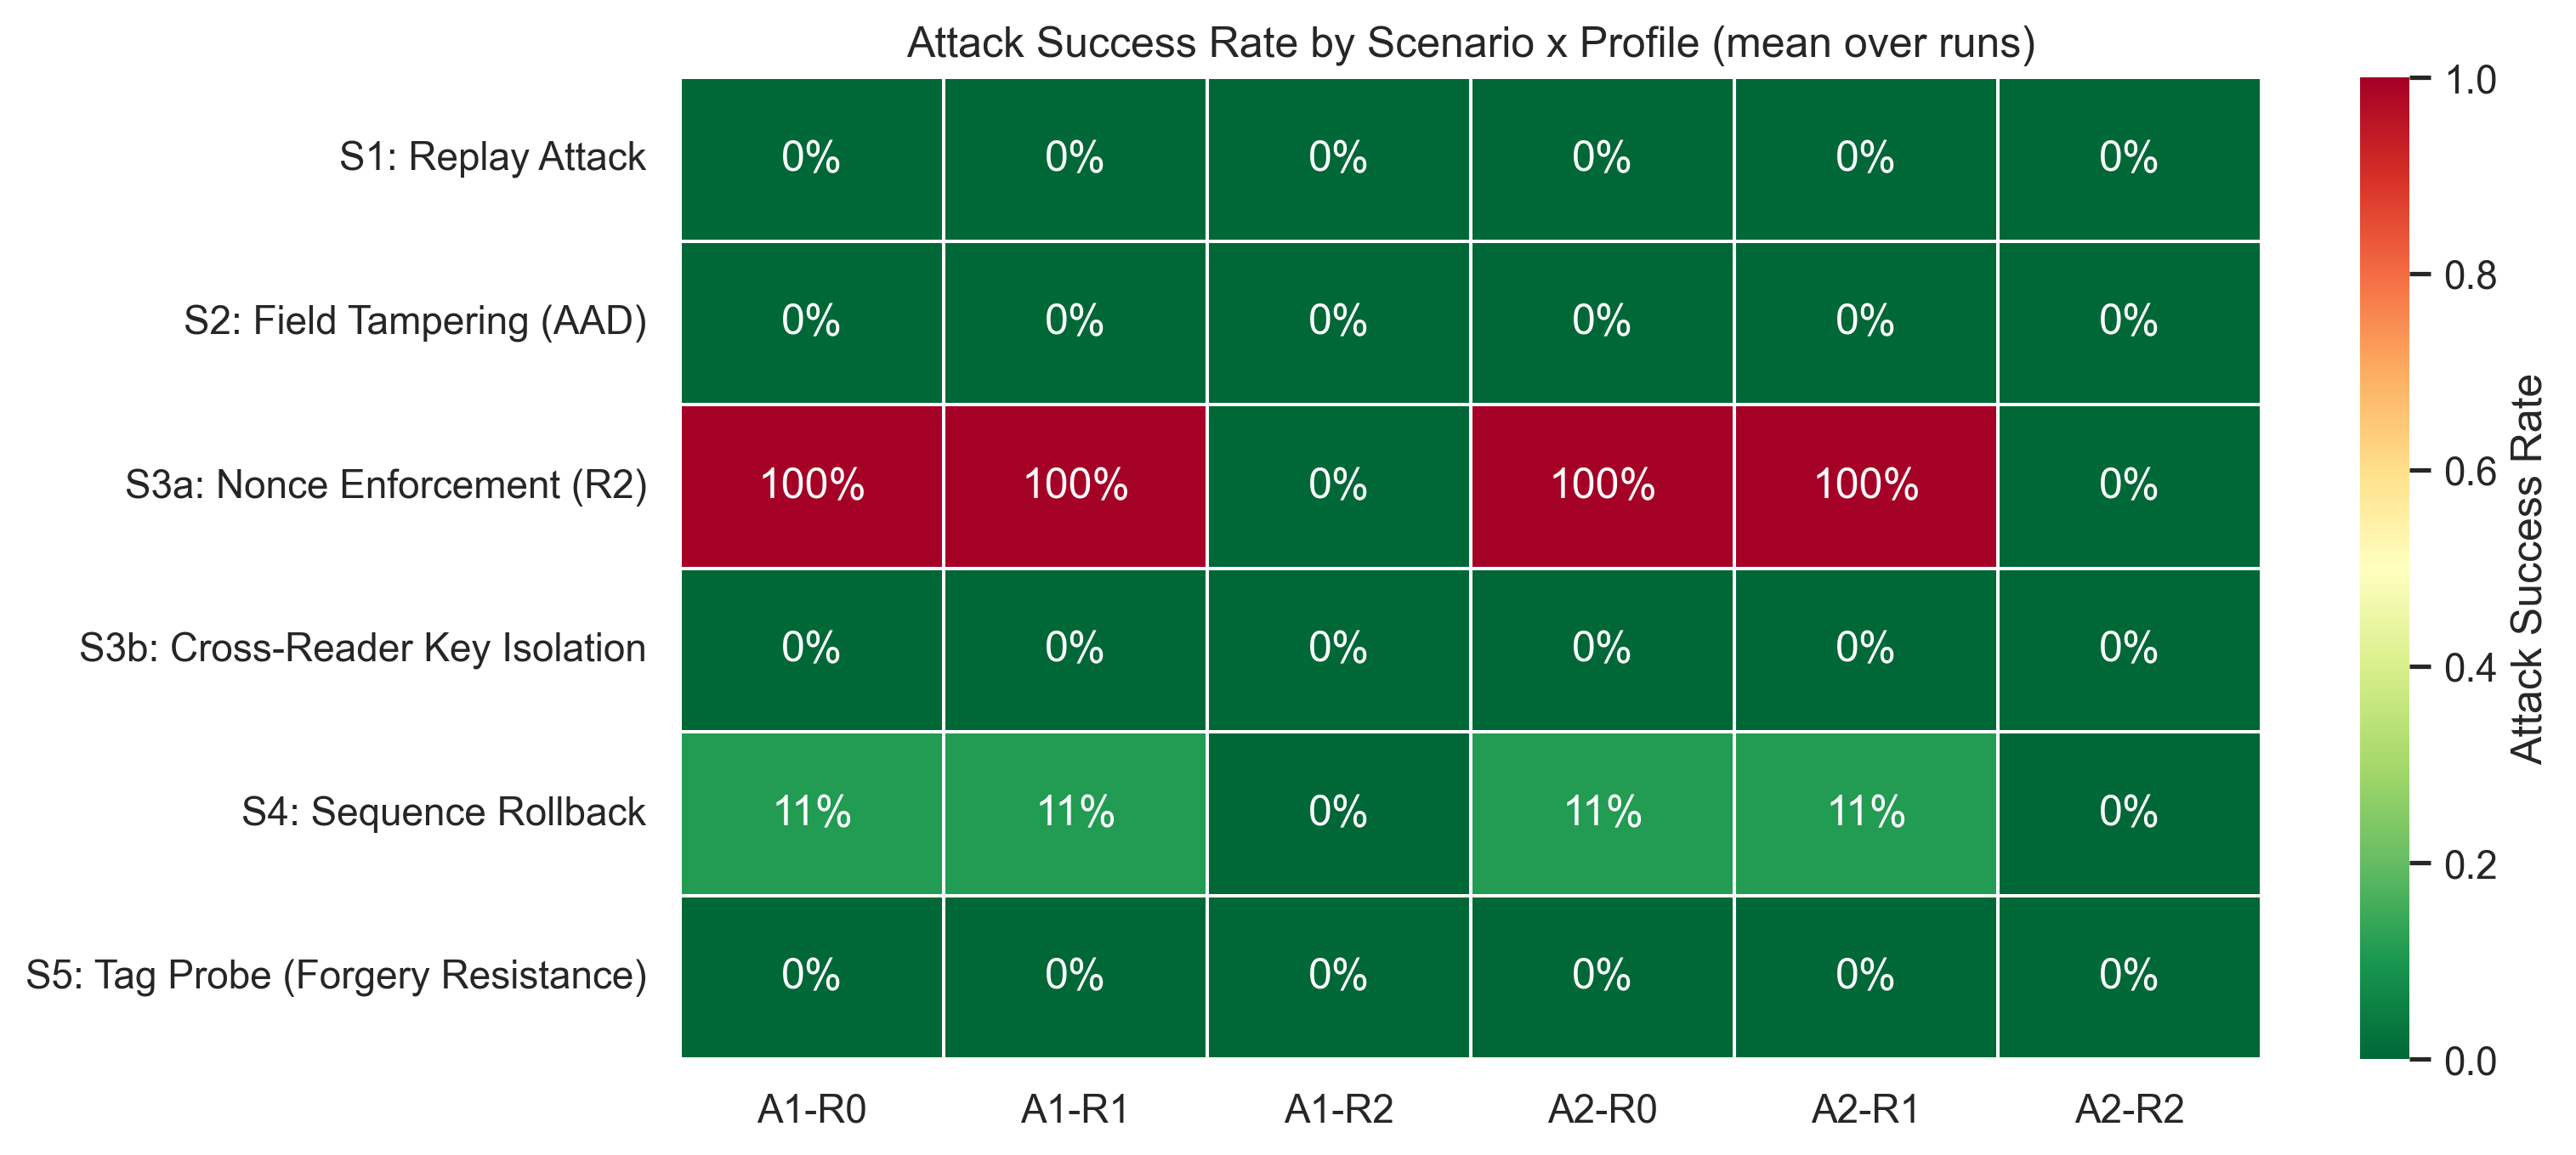
\includegraphics[width=\linewidth]{plots/attack_success_heatmap.png}
\caption{Úspešnosť útokov podľa scenára a profilu (priemer cez 5 behov). Zelené bunky: útok zablokovaný (0\%). Červené bunky: útok úspešný.}
\label{fig:heatmap}
\end{figure}

\begin{table}[htbp]
\centering
\caption{Attack success rate and detector response by scenario and profile}
\label{tab:scenario-summary}
\small
\begin{tabular}{l l r c l l}
\toprule
Scenario & Profile & Success \% & Quarantine & Reason & Anomaly \\
\midrule
  S1: Replay Attack & A1--R0 & 0\% & No & \texttt{replay} & \texttt{--} \\
   & A1--R1 & 0\% & No & \texttt{replay} & \texttt{--} \\
   & A1--R2 & 0\% & Yes & \texttt{quarantined} & \texttt{seq\_reuse} \\
   & A2--R0 & 0\% & No & \texttt{replay} & \texttt{--} \\
   & A2--R1 & 0\% & No & \texttt{replay} & \texttt{--} \\
   & A2--R2 & 0\% & Yes & \texttt{quarantined} & \texttt{seq\_reuse} \\
\midrule
  S2: Field Tampering (AAD) & A1--R0 & 0\% & No & \texttt{decrypt\_failed} & \texttt{--} \\
   & A1--R1 & 0\% & No & \texttt{decrypt\_failed} & \texttt{--} \\
   & A1--R2 & 0\% & Yes & \texttt{quarantined} & \texttt{nonce\_mismatch} \\
   & A2--R0 & 0\% & No & \texttt{decrypt\_failed} & \texttt{--} \\
   & A2--R1 & 0\% & No & \texttt{decrypt\_failed} & \texttt{--} \\
   & A2--R2 & 0\% & Yes & \texttt{quarantined} & \texttt{nonce\_mismatch} \\
\midrule
  S3a: Nonce Enforcement (R2) & A1--R0 & 100\% & No & \texttt{ok} & \texttt{--} \\
   & A1--R1 & 100\% & No & \texttt{ok} & \texttt{--} \\
   & A1--R2 & 0\% & Yes & \texttt{quarantined} & \texttt{nonce\_mismatch} \\
   & A2--R0 & 100\% & No & \texttt{ok} & \texttt{--} \\
   & A2--R1 & 100\% & No & \texttt{ok} & \texttt{--} \\
   & A2--R2 & 0\% & Yes & \texttt{quarantined} & \texttt{nonce\_mismatch} \\
\midrule
  S3b: Cross-Reader Key Isolation & A1--R0 & 0\% & No & \texttt{decrypt\_failed} & \texttt{--} \\
   & A1--R1 & 0\% & No & \texttt{decrypt\_failed} & \texttt{--} \\
   & A1--R2 & 0\% & Yes & \texttt{quarantined} & \texttt{nonce\_mismatch} \\
   & A2--R0 & 0\% & No & \texttt{decrypt\_failed} & \texttt{--} \\
   & A2--R1 & 0\% & No & \texttt{decrypt\_failed} & \texttt{--} \\
   & A2--R2 & 0\% & Yes & \texttt{quarantined} & \texttt{nonce\_mismatch} \\
\midrule
  S4: Sequence Rollback & A1--R0 & 11\% & No & \texttt{replay} & \texttt{--} \\
   & A1--R1 & 11\% & No & \texttt{replay} & \texttt{--} \\
   & A1--R2 & 0\% & Yes & \texttt{quarantined} & \texttt{seq\_rollback} \\
   & A2--R0 & 11\% & No & \texttt{replay} & \texttt{--} \\
   & A2--R1 & 11\% & No & \texttt{replay} & \texttt{--} \\
   & A2--R2 & 0\% & Yes & \texttt{quarantined} & \texttt{seq\_rollback} \\
\midrule
  S5: Tag Probe (Forgery Resistance) & A1--R0 & 0\% & No & \texttt{decrypt\_failed} & \texttt{--} \\
   & A1--R1 & 0\% & No & \texttt{decrypt\_failed} & \texttt{--} \\
   & A1--R2 & 0\% & Yes & \texttt{quarantined} & \texttt{--} \\
   & A2--R0 & 0\% & No & \texttt{decrypt\_failed} & \texttt{--} \\
   & A2--R1 & 0\% & No & \texttt{decrypt\_failed} & \texttt{--} \\
   & A2--R2 & 0\% & Yes & \texttt{quarantined} & \texttt{--} \\
\bottomrule
\end{tabular}
\end{table}

\noindent Z tabuľky~\ref{tab:scenario-summary} a obrázka~\ref{fig:heatmap} vyplýva jasné delenie:

\begin{itemize}[leftmargin=*,itemsep=2pt]
  \item \textbf{S1, S2, S5} --- pri žiadnom profile nedošlo k prijatiu škodlivého frame (0\% úspešnosť). Ochranu zabezpečuje replay window (S1), AAD binding (S2) a AEAD tag verifikácia (S5).
  \item \textbf{S3a} --- nonce enforcement: R0/R1 prepustia frame s chybným nonce (100\%); R2 odchýlku zachytí a zakaranténuje (0\%).
  \item \textbf{S3b} --- cross-reader key isolation: žiadny profil neprijal frame z kontextu inej čítačky (0\%); R2 karanténuje od prvého frame.
  \item \textbf{S4} --- R0/R1 čiastočne zraniteľné (11\%), R2 blokuje (0\%).
\end{itemize}

\subsubsection{Závislosť od počtu útočných frame}

Obrázok~\ref{fig:by_n} zobrazuje ako sa úspešnosť útoku mení s rastúcim $N$. Pásma zobrazujú 95\% interval spoľahlivosti cez 5 behov; nulová šírka pásiem potvrdzuje konzistentnosť výsledkov naprieč všetkými behmi.

\begin{figure}[htbp]
\centering
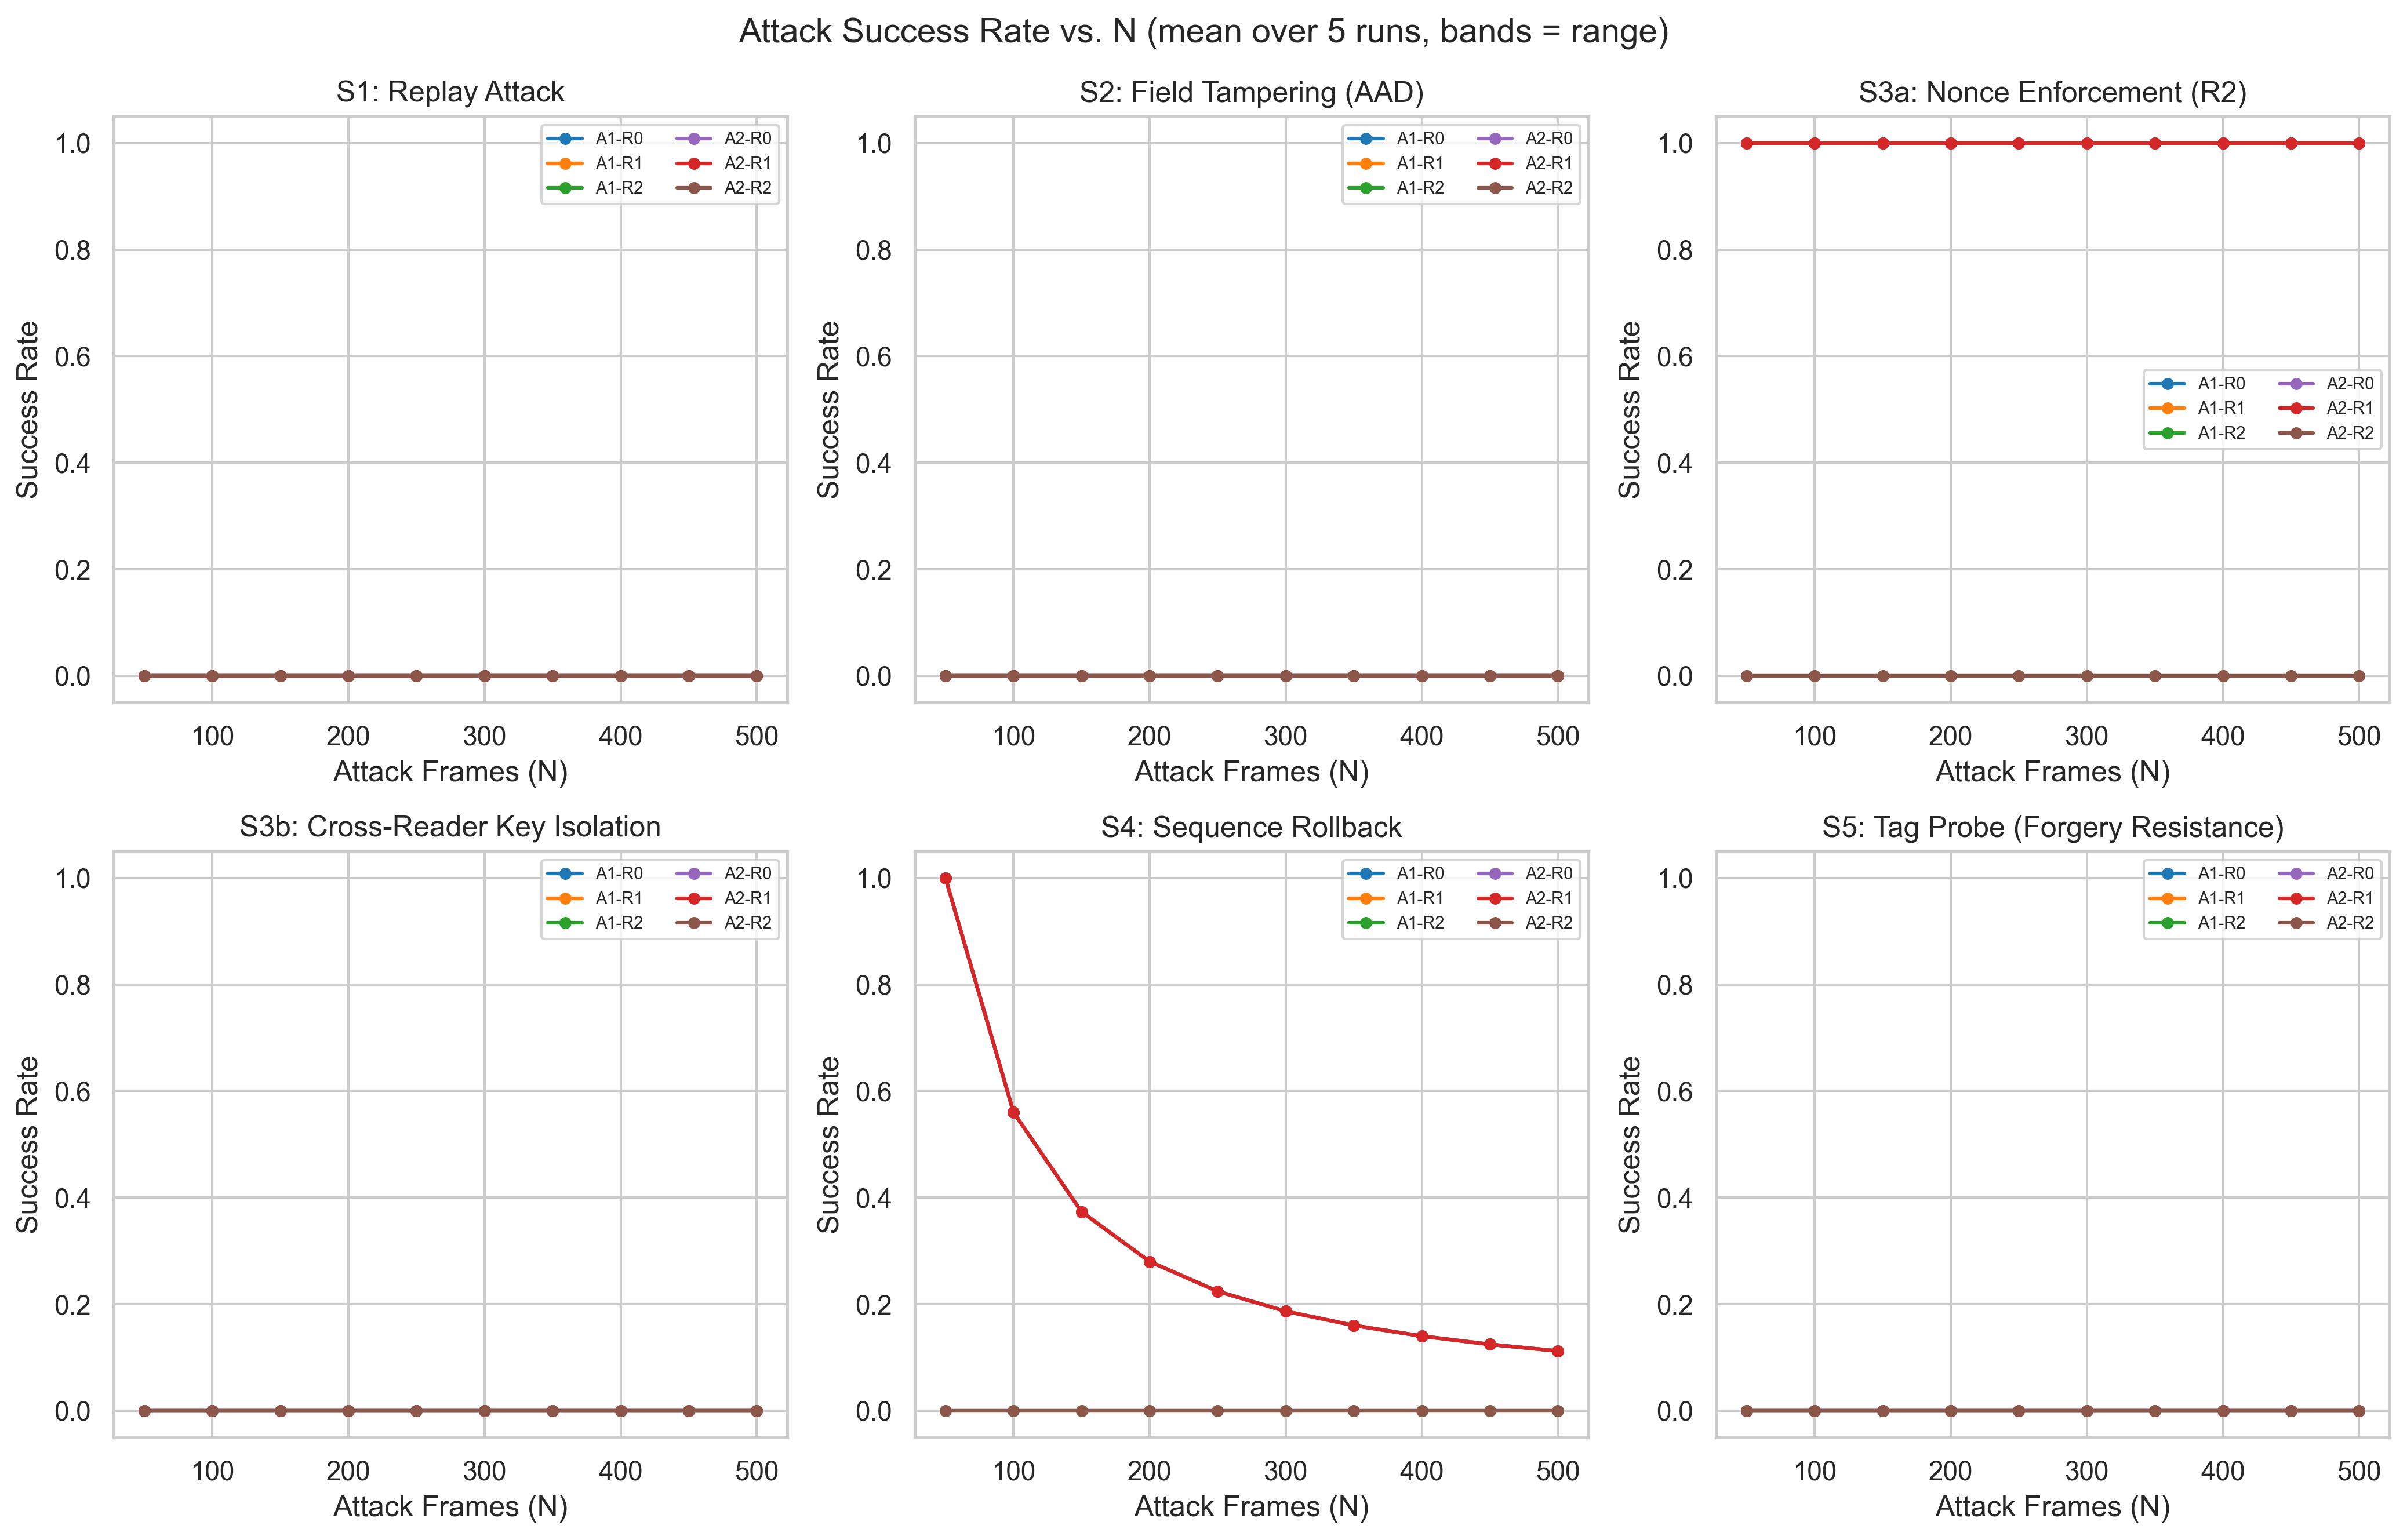
\includegraphics[width=\linewidth]{plots/attack_success_by_n.png}
\caption{Závislosť úspešnosti útoku od počtu útočných frame $N$. Pásma: 95\% CI cez 5 behov (nulová šírka = konzistentný deterministický výsledok).}
\label{fig:by_n}
\end{figure}

\noindent Najzaujímavejší je graf S4 (Sequence Rollback): úspešnosť R0/R1 klesá z ${\sim}100\%$ pri $N=50$ na ${\sim}11\%$ pri $N=500$, pretože rollback zóna obsahuje len 56 unikátnych sekvencií --- po ich vyčerpaní replay window odchytáva opakované hodnoty. R2 profily vykazujú konštantnú nulovú úspešnosť pre všetky $N$.

\subsubsection{Rýchlosť karantény}

\begin{figure}[htbp]
\centering
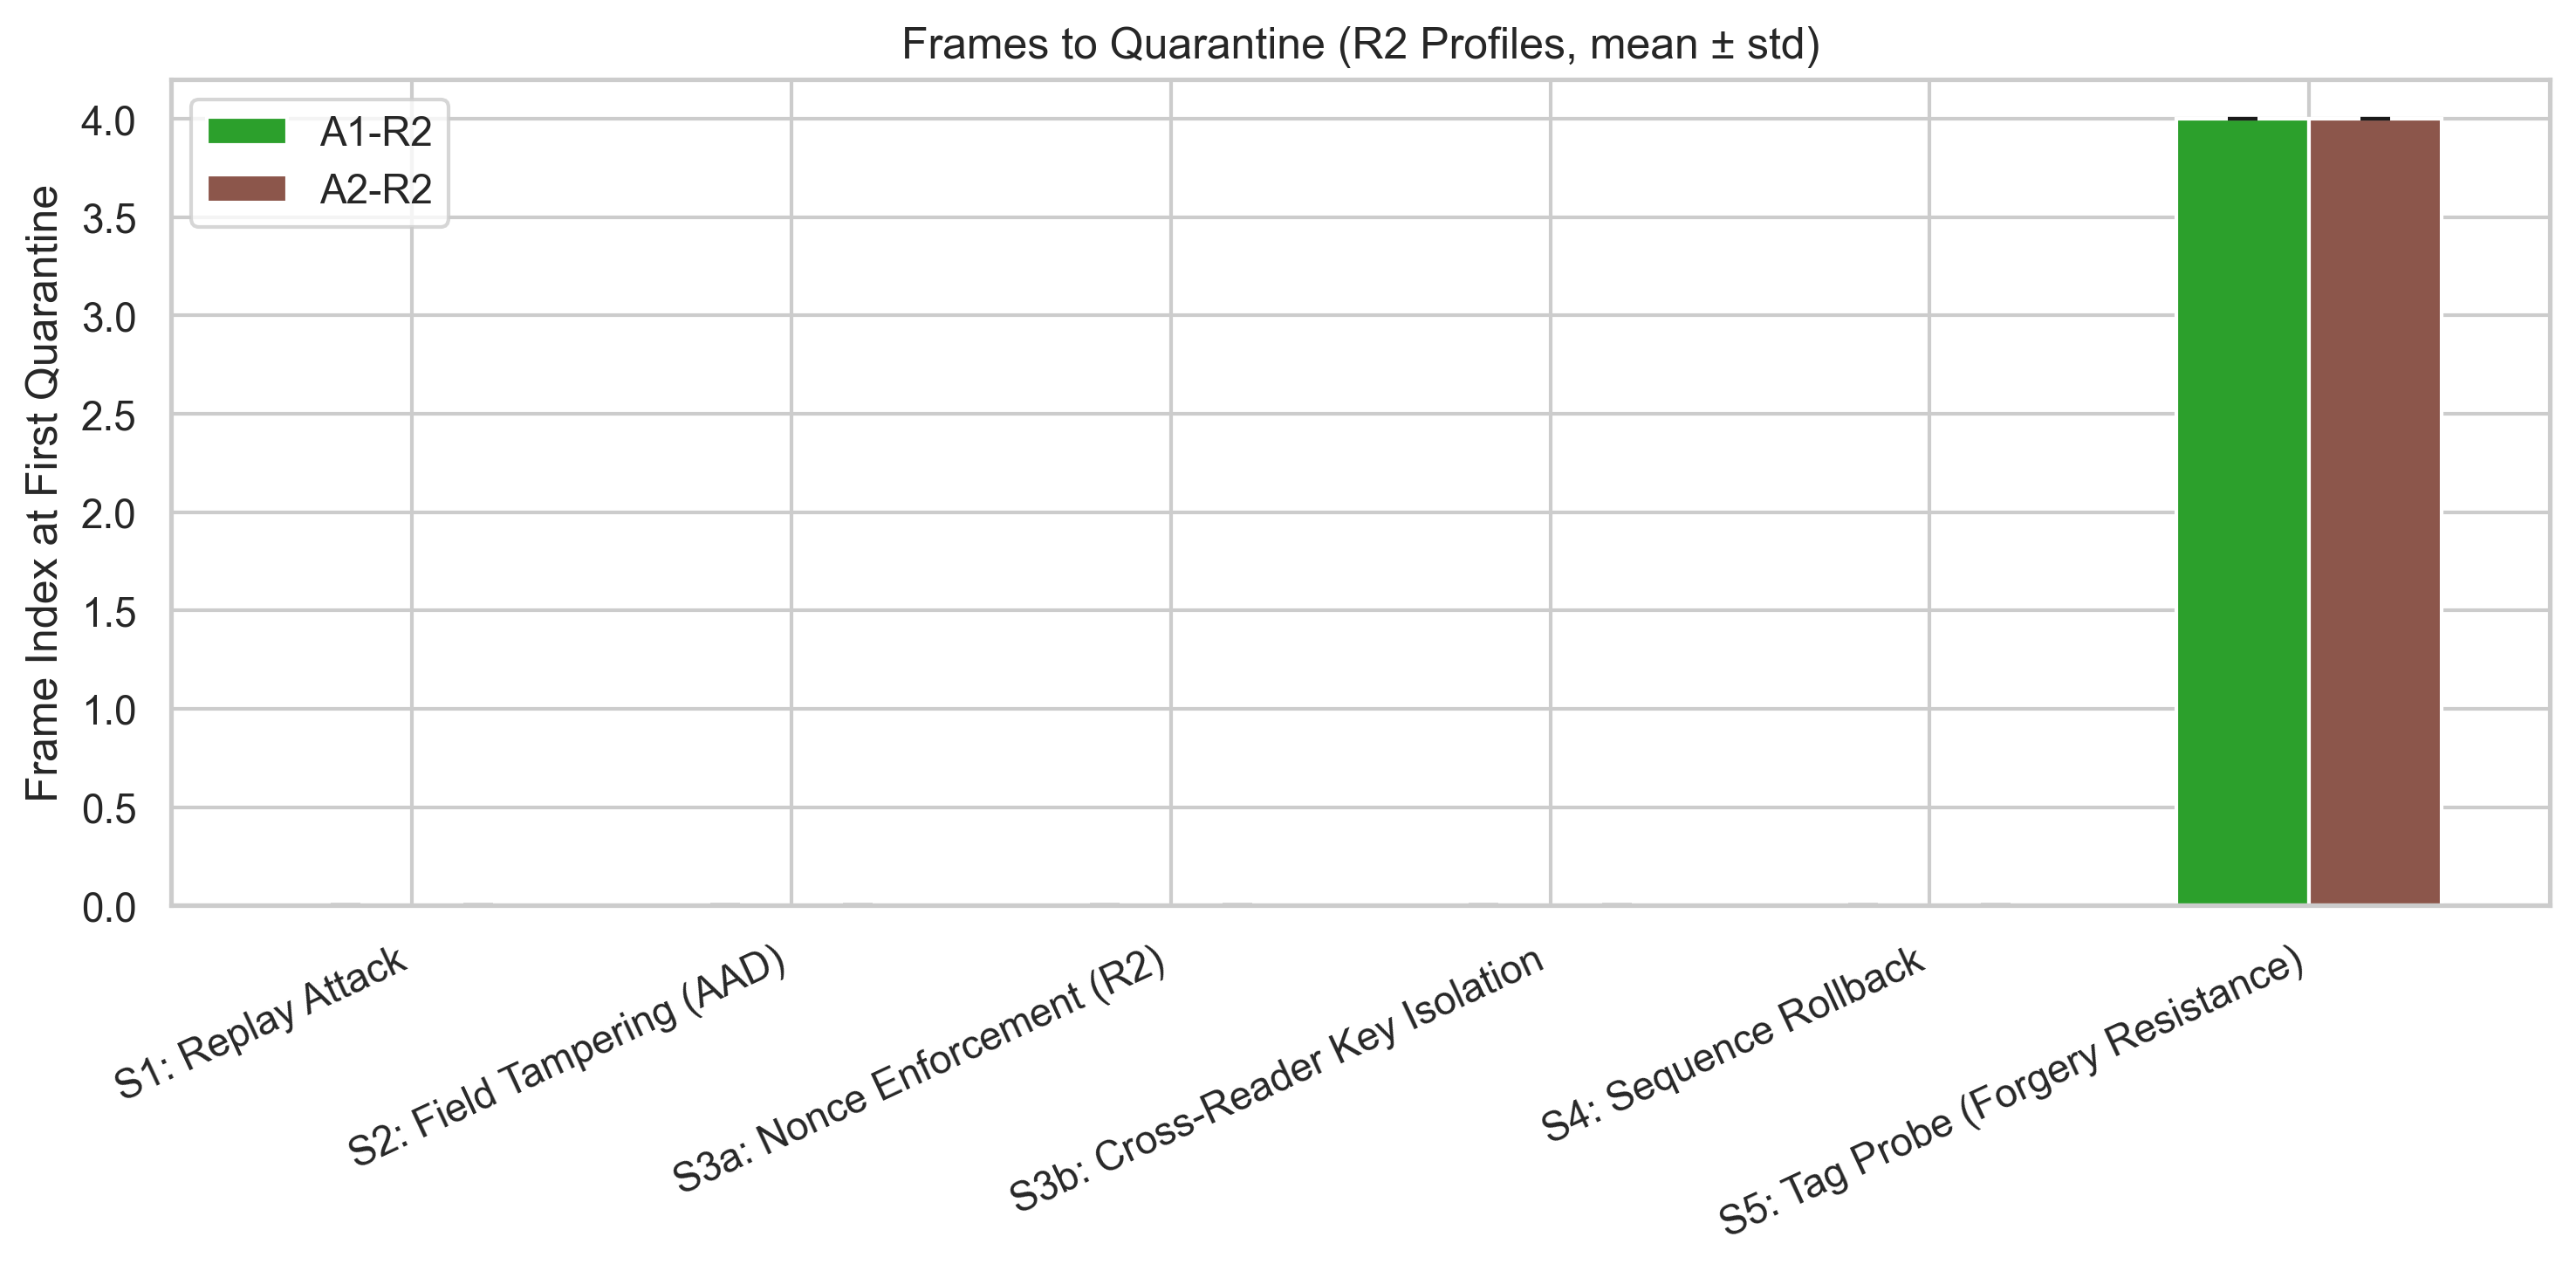
\includegraphics[width=\linewidth]{plots/quarantine_speed.png}
\caption{Počet frame od začiatku útoku do prvej karantény (len R2 profily, priemer $\pm$ std).}
\label{fig:quarantine}
\end{figure}

Obrázok~\ref{fig:quarantine} ukazuje, že pre scenáre S1--S4 nastáva karanténa \emph{na prvom útočnom frame} (frame\_idx = 0). Pre S5 (tag probe) nastáva na frame\_idx = 4, čo zodpovedá nakonfigurovanému limitu \texttt{tag\_fail\_streak\_limit} = 5 (prvé 4 zlyhania sú tolerované; 5.\ zlyhanie aktivuje karanténu). Hodnoty A1--R2 a A2--R2 sú identické, čo potvrdzuje, že rýchlosť detekcie závisí od konfigurácie detektora, nie od zvoleného šifrovacieho algoritmu.

\subsection{Výsledky: Baseline korektnosť}
\label{sec:results_baseline}

\begin{table}[htbp]
\centering
\caption{False reject rate during baseline (valid frames)}
\label{tab:baseline}
\begin{tabular}{l r r r r r r}
\toprule
Scenario & A1--R0 & A1--R1 & A1--R2 & A2--R0 & A2--R1 & A2--R2 \\
\midrule
  S1: Replay Attack & 0.00\% & 0.00\% & 0.00\% & 0.00\% & 0.00\% & 0.00\% \\
  S2: Field Tampering (AAD) & 0.00\% & 0.00\% & 0.00\% & 0.00\% & 0.00\% & 0.00\% \\
  S3a: Nonce Enforcement (R2) & 0.00\% & 0.00\% & 0.00\% & 0.00\% & 0.00\% & 0.00\% \\
  S3b: Cross-Reader Key Isolation & 0.00\% & 0.00\% & 0.00\% & 0.00\% & 0.00\% & 0.00\% \\
  S4: Sequence Rollback & 0.00\% & 0.00\% & 0.00\% & 0.00\% & 0.00\% & 0.00\% \\
  S5: Tag Probe (Forgery Resistance) & 0.00\% & 0.00\% & 0.00\% & 0.00\% & 0.00\% & 0.00\% \\
\bottomrule
\end{tabular}
\end{table}

\noindent Tabuľka~\ref{tab:baseline} potvrdzuje \textbf{nulovú false reject rate} naprieč všetkými scenármi a profilmi. Žiadny validný frame nebol zamietnutý. Toto je nevyhnutná podmienka pre vierohodnosť bezpečnostných výsledkov --- ak by baseline vykazoval falošné odmietnutia, nebolo by možné jednoznačne interpretovať úspešnosť útokov.

\subsection{Výsledky: Latencia a priepustnosť}
\label{sec:results_throughput}

\subsubsection{Throughput benchmark (S6)}

\begin{figure}[htbp]
\centering
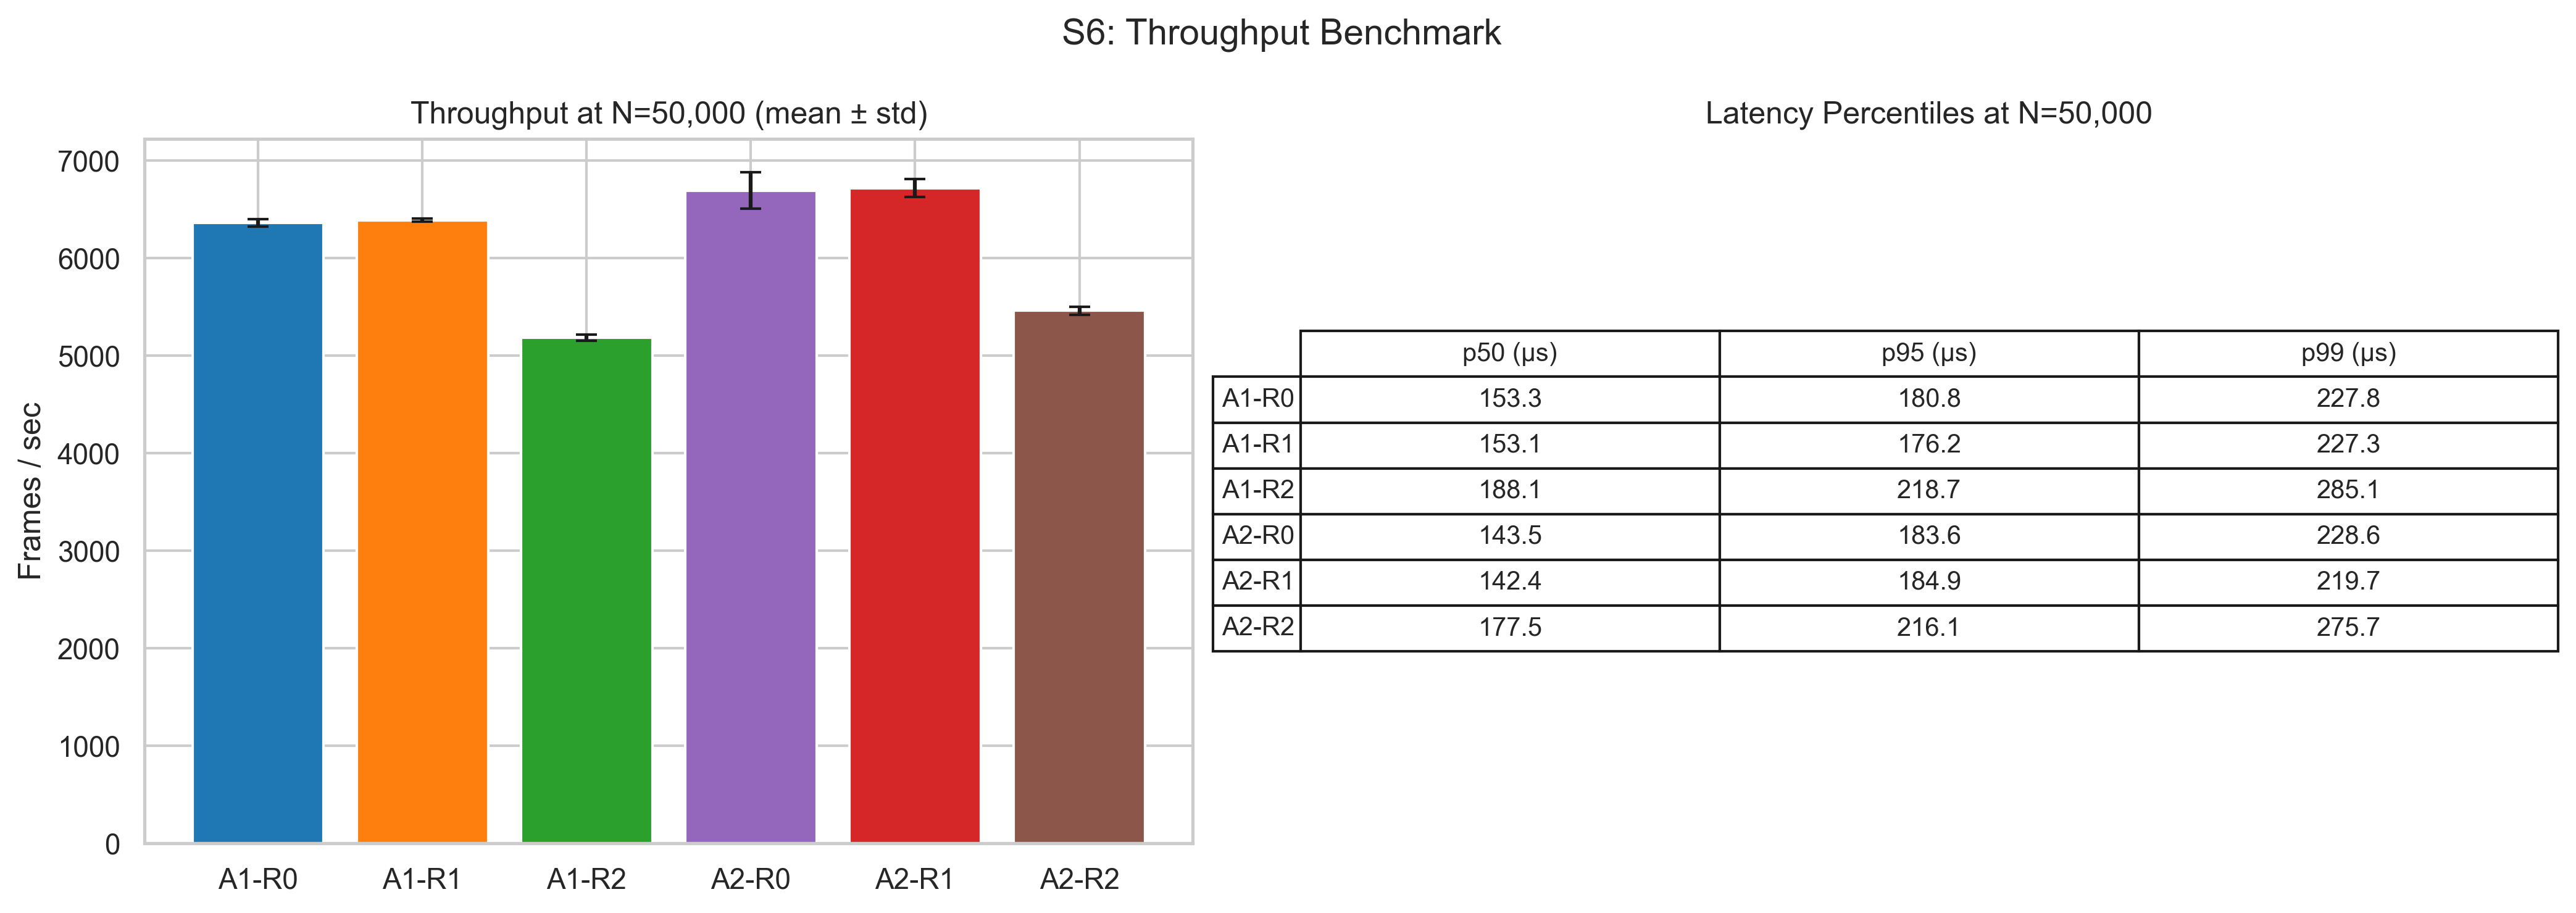
\includegraphics[width=\linewidth]{plots/throughput.png}
\caption{Priepustnosť pri $N=50{,}000$ frame (priemer $\pm$ std cez 5 behov) a percentily latencie.}
\label{fig:throughput}
\end{figure}

\begin{table}[htbp]
\centering
\caption{Throughput and latency at N=50,000 frames}
\label{tab:throughput}
\begin{tabular}{l r r r r r}
\toprule
Profile & FPS (mean) & FPS (std) & p50 ($\mu$s) & p95 ($\mu$s) & p99 ($\mu$s) \\
\midrule
  A1--R0 & 14,284 & 274 & 59.3 & 109.6 & 117.2 \\
  A1--R1 & 16,014 & 680 & 58.4 & 92.3 & 111.5 \\
  A1--R2 & 15,154 & 210 & 62.7 & 88.3 & 113.8 \\
  A2--R0 & 16,529 & 72 & 56.6 & 87.1 & 105.4 \\
  A2--R1 & 17,015 & 67 & 56.7 & 72.2 & 95.9 \\
  A2--R2 & 15,306 & 164 & 62.5 & 86.1 & 106.9 \\
\bottomrule
\end{tabular}
\end{table}

\noindent Obrázok~\ref{fig:throughput} zobrazuje distribúciu priepustnosti pre každý profil. Všetky profily dosahujú priepustnosť nad 5{,}000 frame/s, čo je rádovo viac ako reálna záťaž fyzického prístupového systému ($<$10 udalostí/s). Mediánová latencia je 142--188\,$\mu$s.

\textbf{Porovnanie algoritmov:} A2 (XChaCha20) dosahuje mierne vyššiu priepustnosť ako A1 (ChaCha20), čo je prekvapivý výsledok. Príčinou je pravdepodobne optimalizácia libsodium pre XChaCha20 cestu.

\textbf{Overhead detektora:} Porovnanie R1 a R2 umožňuje izolovať overhead \texttt{ProtocolAnomalyDetector}. Rozdiel je ${\sim}19\%$ (A2--R1: 6{,}720~fps vs.\ A2--R2: 5{,}462~fps). Tento overhead pochádza z:
\begin{itemize}[leftmargin=*,itemsep=1pt]
  \item výpočtu očakávaného nonce (HKDF derivácia + HMAC),
  \item porovnania nonce v konštantnom čase (\texttt{sodium\_memcmp}),
  \item aktualizácie stavu detektora (rollback check, tag streak).
\end{itemize}

\subsubsection{Overhead detektora na baseline frame}

\begin{figure}[htbp]
\centering
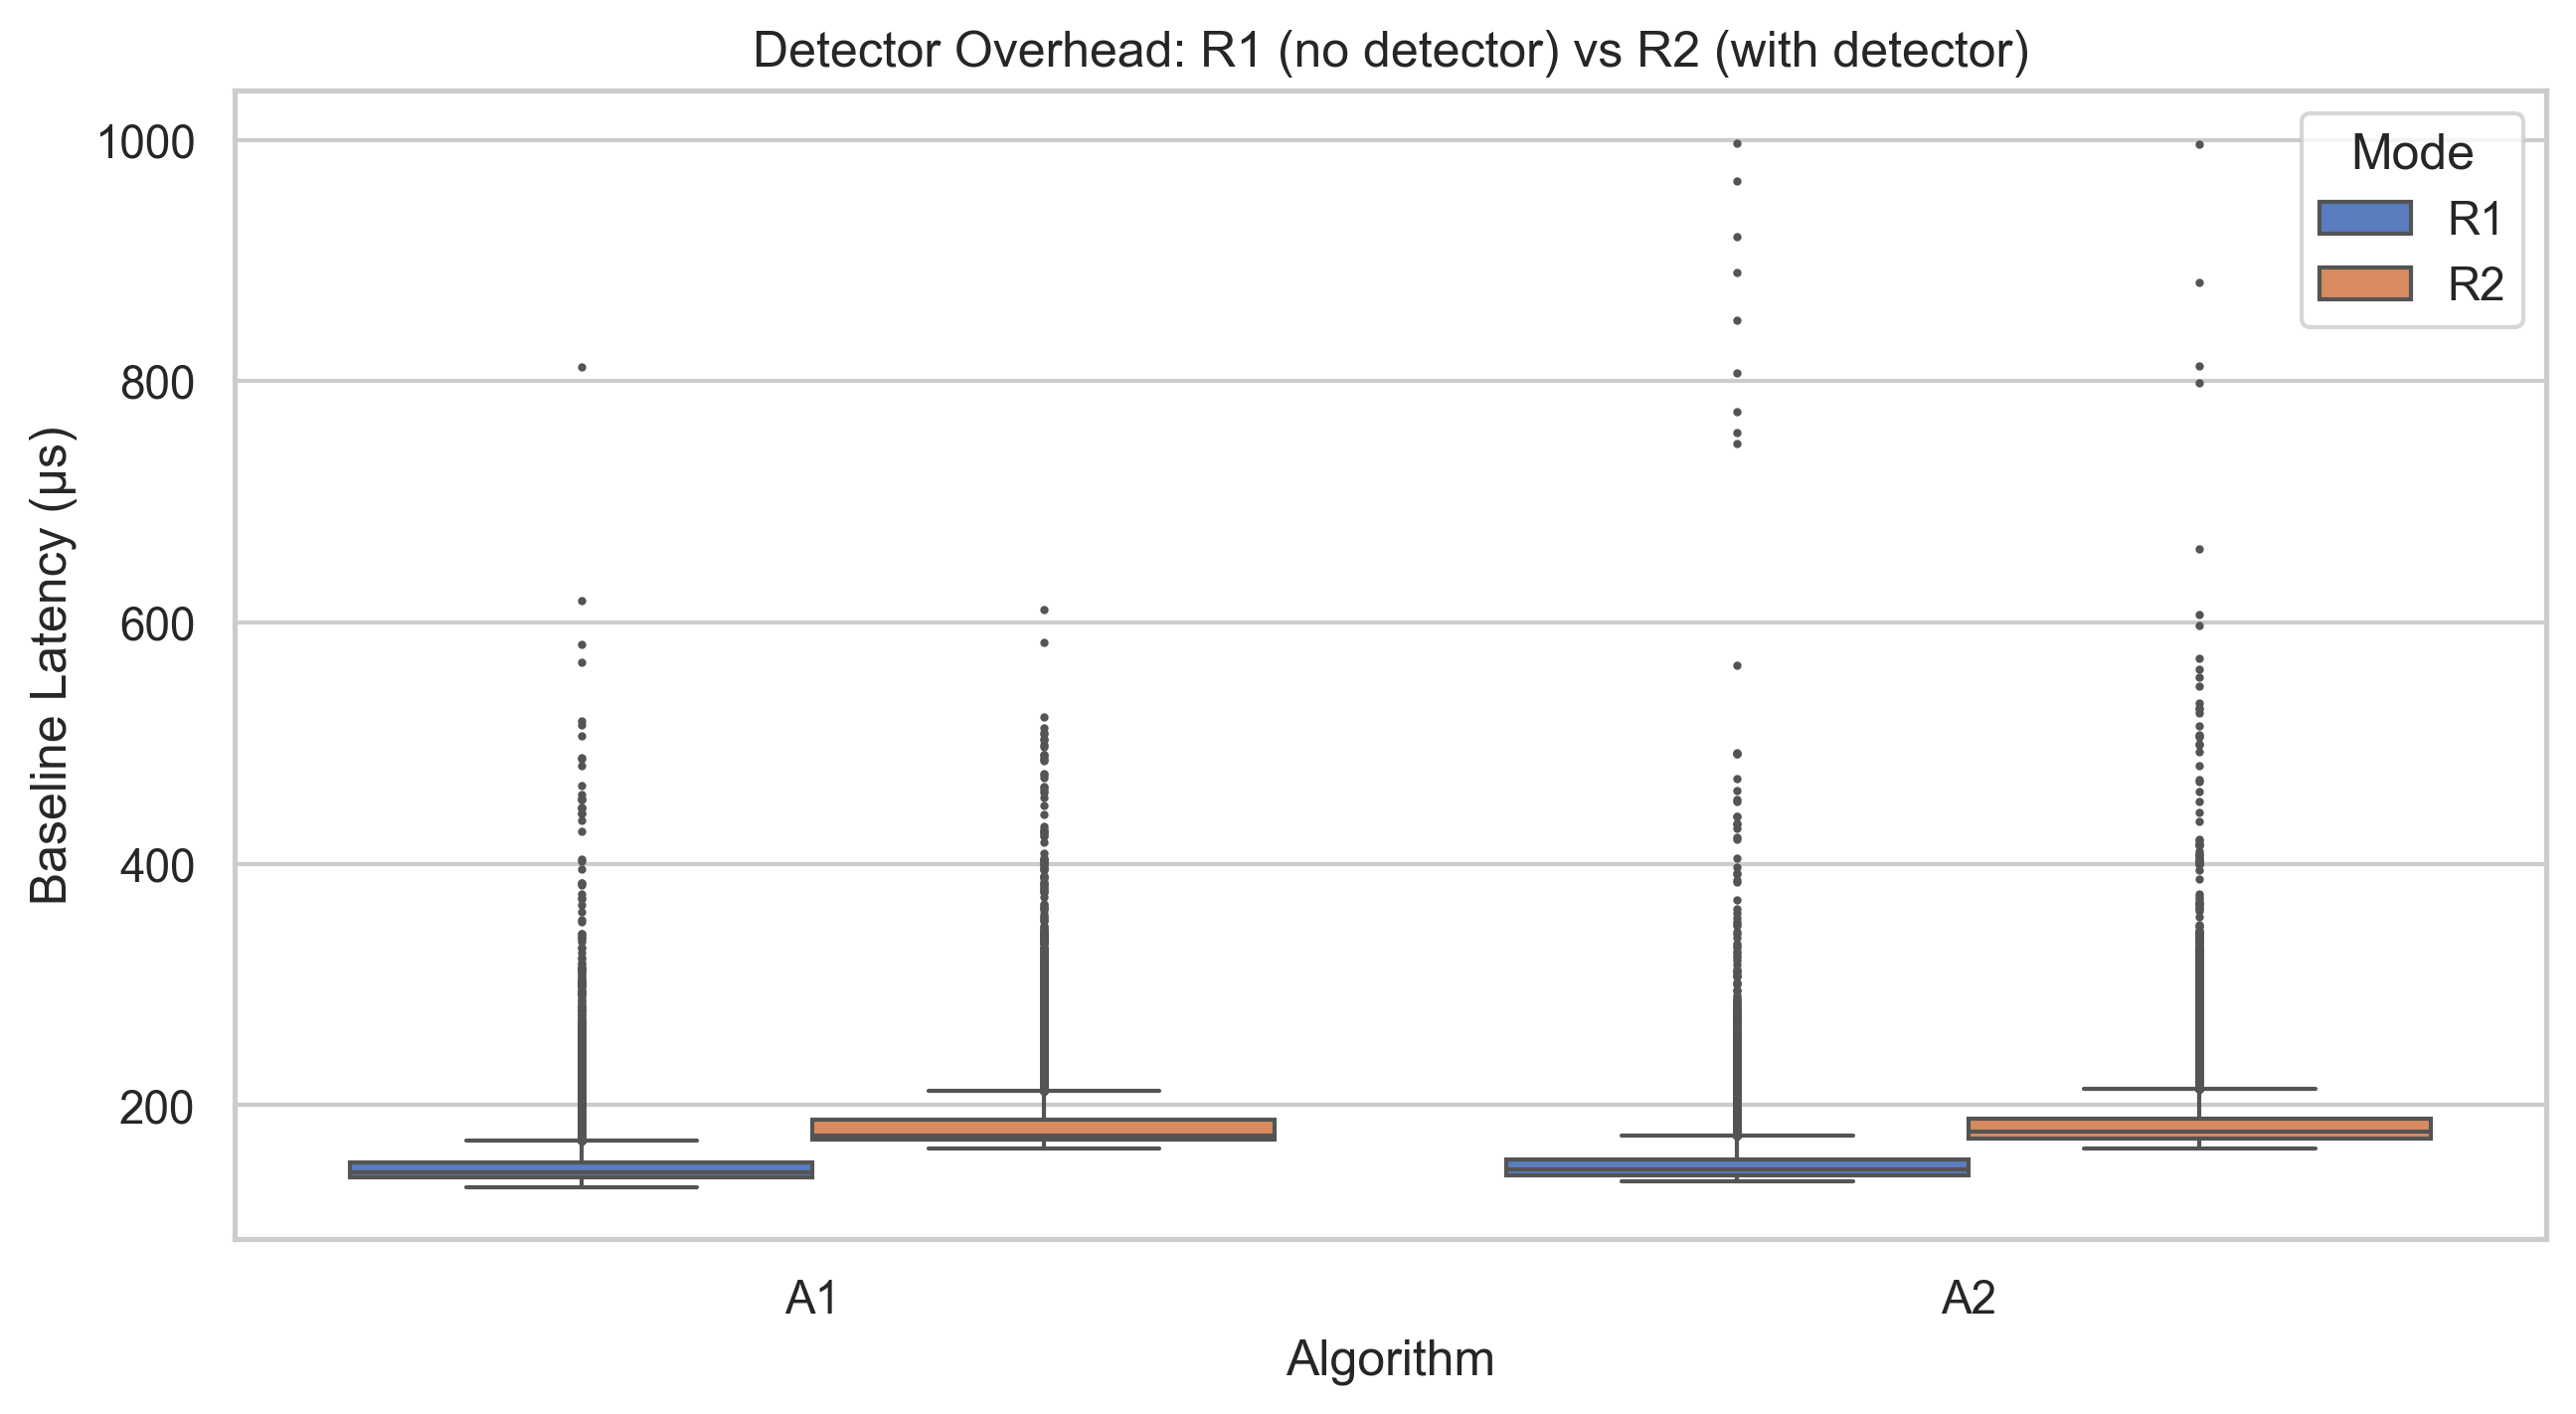
\includegraphics[width=\linewidth]{plots/detector_overhead.png}
\caption{Porovnanie latencie R1 (bez detektora) a R2 (s detektorom) na validných baseline frame.}
\label{fig:overhead}
\end{figure}

\noindent Obrázok~\ref{fig:overhead} izoluje overhead detektora porovnaním R1 a R2 na baseline frame z S1--S5. Medián latencie R2 je o ${\sim}35\,\mu$s vyšší, čo zodpovedá dodatočnej HKDF derivácii nonce kľúča, HMAC výpočtu pre overenie nonce a aktualizácii stavu detektora.

\subsubsection{Distribúcia latencie podľa scenárov}

\begin{figure}[htbp]
\centering
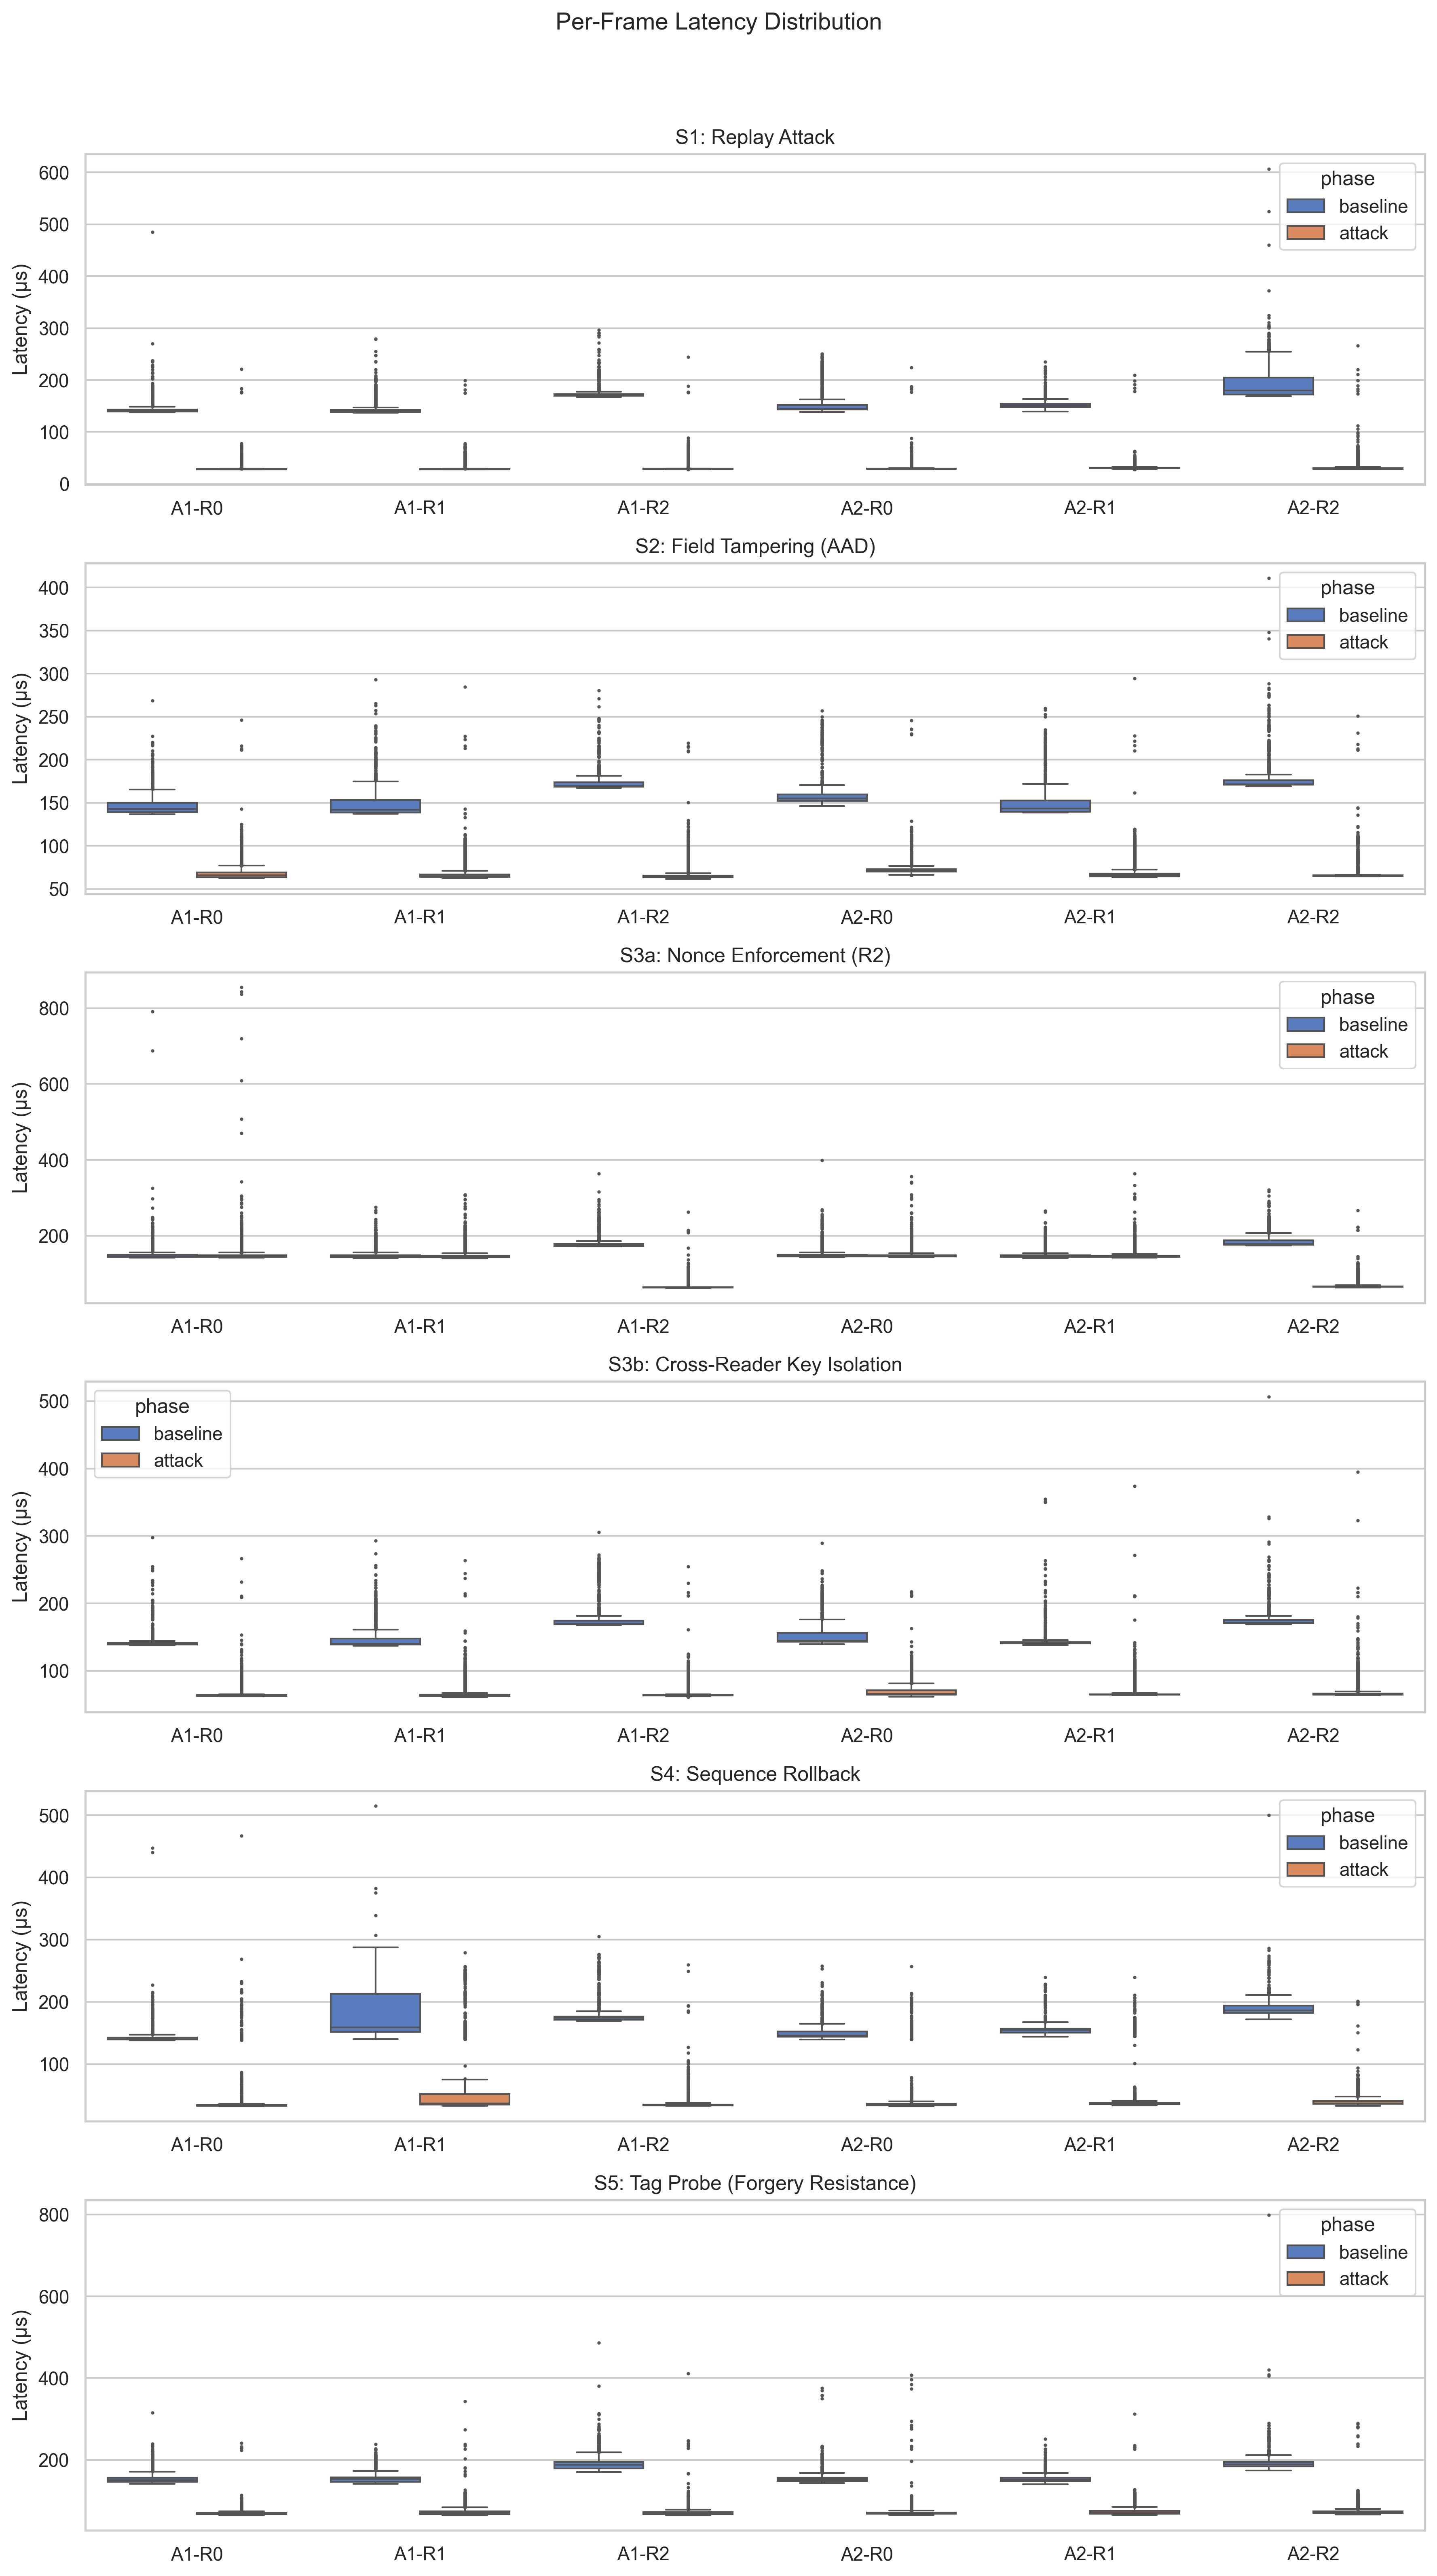
\includegraphics[width=\linewidth]{plots/latency_boxplot.png}
\caption{Distribúcia latencie podľa scenára a profilu (baseline vs.\ attack fáza, $N=500$).}
\label{fig:latency}
\end{figure}

\noindent Obrázok~\ref{fig:latency} zobrazuje boxploty latencie pre každý scenár. Viditeľný je rozdiel medzi baseline a attack fázou: pri S1 (replay) je attack latencia nižšia, pretože replay window odmietne frame skôr bez pokusu o dešifrovanie. Pri S2 a S5 je attack latencia vyššia pre R2, pretože detektor vykonáva dodatočné kontroly pred zamietnutím.

\subsection{Diskusia a interpretácia výsledkov}
\label{sec:discussion}

\subsubsection{Tézis 1: Nonce enforcement a HKDF izolácia ako dva piliere bezpečnosti}

\textbf{S3a --- nonce enforcement:} R0/R1 nemajú verifikáciu nonce; frame s chybným nonce prejde so 100\% úspešnosťou. R2 rekonštruuje očakávaný nonce a pri nesúlade okamžite zakaranténuje čítačku (0\% úspešnosť). S3a je jediný scenár, kde sa R0/R1 a~R2 správajú zásadne odlišne. V~aktuálnom jednoserverovom nasadení generátor a~verifikátor nonce zdieľajú ten istý \texttt{KeyManager} --- odchýlka nemôže nastať za normálnych okolností. Ak však systém prejde na distribuovanú architektúru (viacero serverov, oddelené generovanie a~verifikácia), vynucovaná nonce politika sa stáva kritickou poistkou proti tichému porušeniu unikátnosti nonce\cite{RogawayNonceMisuse2004}.

\textbf{S3b --- HKDF key isolation:} HKDF\cite{RFC5869} derivuje unikátny AEAD kľúč pre každú kombináciu (reader\_id, key\_version). Žiadny profil neprijal ani jeden cross-reader frame (0\% úspešnosť). R2 reaguje okamžitou karanténou (nonce kontextový nesúlad), R0/R1 odmietajú individuálne (decrypt\_failed).

\textbf{Záver:} S3a a~S3b testujú dve komplementárne osi bezpečnosti. Nonce enforcement (S3a) diferencuje nonce režimy a~zabezpečuje škálovateľnosť; HKDF izolácia (S3b) zabezpečuje compartmentalization medzi čítačkami nezávisle od nonce režimu.

\subsubsection{Tézis 2: ProtocolAnomalyDetector materiálne zvyšuje bezpečnosť}

R2 profily dosiahli 0\% úspešnosť útoku naprieč všetkými testovanými scenármi. V scenároch S3a a S4 bol R2 \textbf{jediným z testovaných mechanizmov}, ktorý útok zastavil:

\begin{itemize}[leftmargin=*,itemsep=2pt]
  \item S3a: nonce enforcement --- R0/R1 prepustia 100\%, R2 zachytí a zakaranténuje (0\%),
  \item S3b: cross-reader --- všetky profily blokujú (HKDF izolácia), R2 navyše karanténuje od prvého frame,
  \item S4: 11\% $\rightarrow$ 0\% (seq\_rollback detekcia).
\end{itemize}

\noindent V S1, S2 a S5 iné mechanizmy (replay window, AAD, AEAD tag verifikácia) tiež zamietajú škodlivé frame, ale R2 pridáva \emph{karanténu} --- čítačka je zablokovaná pre ďalšie požiadavky, nielen odmietnutý jednotlivý frame.

\textbf{Záver:} \texttt{ProtocolAnomalyDetector} nie je len doplnok k existujúcim mechanizmom. V~dvoch z~piatich testovaných útokových scenárov (S3a, S4) bol jedinou testovanou ochranou; v~S3b a~S5 pridáva operačnú eskaláciu (karanténu) k~existujúcemu kryptografickému odmietnutiu.

\subsubsection{Tézis 3: Replay window a anomálna detekcia sú komplementárne}

Scenár S4 demonštruje štruktúrnu medzeru replay window. Funkcia \texttt{ReplayWindow::contains()} kontroluje:

\begin{equation}
\text{contains}(\text{seq}) = \text{isTooOld}(\text{seq}) \lor (\text{seq} \in \text{\_seen})
\end{equation}

\noindent kde $\text{isTooOld}(\text{seq}) = (\text{seq} \leq \text{maxSeen} - W)$. Sekvenčné čísla v rollback zóne:

\begin{itemize}[leftmargin=*,itemsep=1pt]
  \item nie sú príliš staré ($> \text{maxSeen} - W$),
  \item nie sú v množine videných (nikdy neboli odoslané).
\end{itemize}

\noindent Replay window ich preto prepustí. Detektor ich zachytí cez podmienku:
\begin{equation}
\text{seq} + \delta < \text{maxSeenSeq} \implies \text{quarantine}(\texttt{seq\_rollback})
\end{equation}

\textbf{Záver:} Replay window a anomálna detekcia chránia pred rôznymi triedami útokov. Replay window odchytáva presné duplikáty. Detektor odchytáva štrukturálne anomálie (rollback, nonce mismatch, brute-force séria). Sú komplementárne, nie ekvivalentné --- v súlade s princípom vrstvených kontrol, kde každý mechanizmus pokrýva odlišnú triedu hrozieb\cite{NIST80053,DefenseInDepth}.

\subsubsection{Tézis 4: AAD binding poskytuje ochranu nezávisle od režimu nonce}

Scenár S2 ukazuje, že manipulácia \texttt{door\_id} je detekovaná \textbf{všetkými} profilmi. Mechanizmus je odlišný:
\begin{itemize}[leftmargin=*,itemsep=2pt]
  \item R0/R1: AEAD tag verification zlyhá, pretože AAD sa zmenilo $\rightarrow$ \texttt{decrypt\_failed}.
  \item R2: Deterministický nonce závisí od \texttt{door\_id} (súčasť header context). Zmena \texttt{door\_id} zmení kontext $\rightarrow$ nonce v hlavičke nezodpovedá $\rightarrow$ \texttt{nonce\_mismatch} (detekcia \emph{pred} dešifrovaním).
\end{itemize}

\textbf{Záver:} AAD binding je fundamentálna ochrana, ktorá funguje nezávisle od konfigurácie nonce a detektora. R2 ju dopĺňa skoršou detekciou.

\subsubsection{Tézis 5: Defense-in-depth cez karanténu}

Aj v scenároch, kde R0/R1 blokujú každý individuálny útočný frame (S1, S5), R2 pridáva kvalitatívne odlišnú reakciu: karanténu celej čítačky. Kým R0/R1 odmietajú frame poštučne (útočník môže pokračovať s ďalšími pokusmi), R2 po prvom detekovanom incidente zablokuje \textbf{všetku} komunikáciu z danej čítačky.

\textbf{Záver:} Karanténa mení reakciu systému z reaktívnej (odmietni frame) na proaktívnu (izoluj zariadenie). Toto je realizácia princípu defense-in-depth\cite{DefenseInDepth} --- vrstvy ochrany nepôsobia len nezávisle, ale eskalujú reakciu pri detekcii závažnejších anomálií. V prístupových systémoch, kde kompromitovaná čítačka môže generovať veľký objem požiadaviek, je izolácia zariadenia kritická\cite{NIST80094}.

\subsubsection{Tézis 6: Overhead detektora je prijateľný}

Tabuľka~\ref{tab:throughput} ukazuje overhead detektora:
\begin{itemize}[leftmargin=*,itemsep=1pt]
  \item A1: R1 (6{,}389~fps) $\rightarrow$ R2 (5{,}188~fps): $-18.8\%$
  \item A2: R1 (6{,}720~fps) $\rightarrow$ R2 (5{,}462~fps): $-18.7\%$
\end{itemize}

\noindent Aj pri najnižšej nameranej priepustnosti (A1--R2: 5{,}188~fps) systém spracuje $>$5{,}000 frame/s. Fyzický prístupový systém typicky generuje menej ako 10 udalostí za sekundu. Overhead detektora (${\sim}19\%$) je teda rádovo nepodstatný pre reálnu prevádzku, hoci nie je zanedbateľný a mal by byť zohľadnený pri nasadení s~vyššou záťažou.

\medskip
\noindent\textbf{Poznámka k porovnaniu A1 a A2.}
Namerané rozdiely v priepustnosti medzi algoritmami A1 (ChaCha20-Poly1305) a A2 (XChaCha20-Poly1305) odrážajú výkon konkrétnych implementácií v knižnici libsodium 1.0.20\cite{LibsodiumDoc}, nie inherentné vlastnosti abstraktných algoritmov. Dva faktory limitujú prenositeľnosť tohto porovnania:

\begin{enumerate}[leftmargin=*,itemsep=2pt]
  \item \textbf{Architektonický overhead XChaCha20.} XChaCha20 vykonáva pred samotným šifrovaním medzikrok HChaCha20\cite{Bernstein2012}, ktorý redukuje 192-bitový nonce na 96-bitový podkľúč. Tento krok pridáva konštantný overhead jedného volania blokovej funkcie. V inej implementácii (napríklad hardvérovom akcelerátori alebo inom softvérovom frameworku) by pomer režijných nákladov mohol byť odlišný.
  \item \textbf{Úroveň optimalizácie.} Libsodium obsahuje ručne optimalizované varianty ChaCha20 pre inštrukčné sady AVX2 a SSSE3 (adresár \texttt{dolbeau/}), ktoré sa aktivujú na platformách s podporou SIMD. Miera optimalizácie nemusí byť identická pre oba algoritmy --- napríklad HChaCha20 nemusí využívať rovnakú úroveň SIMD vektorizácie ako hlavný ChaCha20 stream. Pozorované rozdiely preto môžu čiastočne odrážať \emph{kvalitu implementácie} v libsodium, nie čistú algoritmickú zložitosť.
\end{enumerate}

\noindent Pre závery tejto práce je toto rozlíšenie nepodstatné: oba algoritmy sú ekvivalentné z hľadiska bezpečnostných metrík (scenáre S1--S5) a oba dosahujú priepustnosť rádovo prevyšujúcu požiadavky fyzického prístupového systému. Avšak pri extrapolácii nameraných výkonnostných údajov na iné platformy alebo iné kryptografické knižnice\cite{OpenSSL,BoringSSL} je potrebné vykonať nezávislé meranie.

\subsection{Porovnanie s minimalistickými implementáciami}
\label{sec:baseline_comparison}

Experimentálna matica pokrýva šesť profilov od A1-R0 po A2-R2. Pre úplnosť kontextu je užitočné zasadiť výsledky do širšieho rámca a porovnať ich s~hypotetickými minimalistickými architektúrami, ktoré sa v~praxi vyskytujú v~jednoduchých prístupových systémoch.

Uvažujeme tri referenčné úrovne ochrany:
\begin{description}[leftmargin=*,itemsep=3pt]
  \item[B0 --- bez kryptografickej ochrany:] HTTP endpoint bez podpisu požiadavky, payload prenášaný ako plaintext, žiadna anti-replay ochrana, žiadny audit.
  \item[B1 --- základný HTTPS:] HTTPS s tokenom v~hlavičke (napr.\ statický API kľúč), ale bez interného AEAD frame, bez anti-replay sekvencie a bez tamper-evident auditu. Bežný vzor pre jednoduché IoT API.
  \item[A1-R0 --- základný profil tejto práce:] Náš najjednoduchší testovaný profil. Pridáva: HMAC podpis každej požiadavky, interný AEAD frame (ChaCha20-Poly1305) s~AAD binding, sliding window anti-replay, pepper-hashed identifikátory kariet a~HMAC hash chain audit.
\end{description}

\begin{table}[htbp]
\renewcommand{\arraystretch}{1.3}
\centering
\caption{Odolnosť voči útočným scenárom podľa úrovne implementácie}
\label{tab:baseline_comparison}
\small
\begin{tabular}{l c c c c}
\toprule
\textbf{Scenár / útok} & \textbf{B0} & \textbf{B1} & \textbf{A1-R0} & \textbf{A1-R2 / A2-R2} \\
\midrule
S1 Replay           & \texttimes & \texttimes  & \checkmark & \checkmark{} + karanténa \\
S2 Tampering (AAD)  & \texttimes & čiastočne   & \checkmark & \checkmark{} (pred dekr.) \\
S3a Nonce enforcement & n/a        & n/a         & \texttimes & \checkmark \\
S3b Cross-reader     & \texttimes & \texttimes  & \checkmark & \checkmark{} + karanténa \\
S4 Seq rollback     & \texttimes & \texttimes  & čiastočne  & \checkmark \\
S5 Tag probe        & \texttimes & \texttimes  & \checkmark & \checkmark{} + karanténa \\
Manipulácia auditu  & \texttimes & \texttimes  & \checkmark & \checkmark \\
Identita karty (DB) & \texttimes & \texttimes  & \checkmark{} (HMAC) & \checkmark \\
\bottomrule
\end{tabular}
\end{table}

Z~tabuľky vyplývajú tri závery. Po prvé, prechod z~B0 na A1-R0 predstavuje kvalitatívny skok: väčšina útočných scenárov (S1, S2, S3, S5, audit, identita) je zastavená bez nutnosti nasadiť R2. Po druhé, plná ochrana pri S4 vyžaduje R2 detektor --- jednoduché AEAD bez anomálnej detekcie nestačí na detekciu seq rollback. Po tretie, karanténa v~R2 profiloch mení charakter odpovede systému z~per-frame odmietania na izoláciu celého zariadenia, čo je realizáciou princípu \emph{defense-in-depth}\cite{DefenseInDepth,NIST80053}.

B1 (HTTPS bez interného AEAD) chráni pred pasívnym odpočúvačom na sieťovej vrstve, no nevyrieši scenáre, kde je komunikácia legitimná na transportnej vrstve ale manipulovaná na aplikačnej --- presne to, čo demonštrujú S1--S5. Interný AEAD frame a~anti-replay sú teda komplementárne k~TLS, nie jeho náhradou\cite{RFC9325}.

\subsection{Zhrnutie experimentov}

\begin{figure}[htbp]
\centering
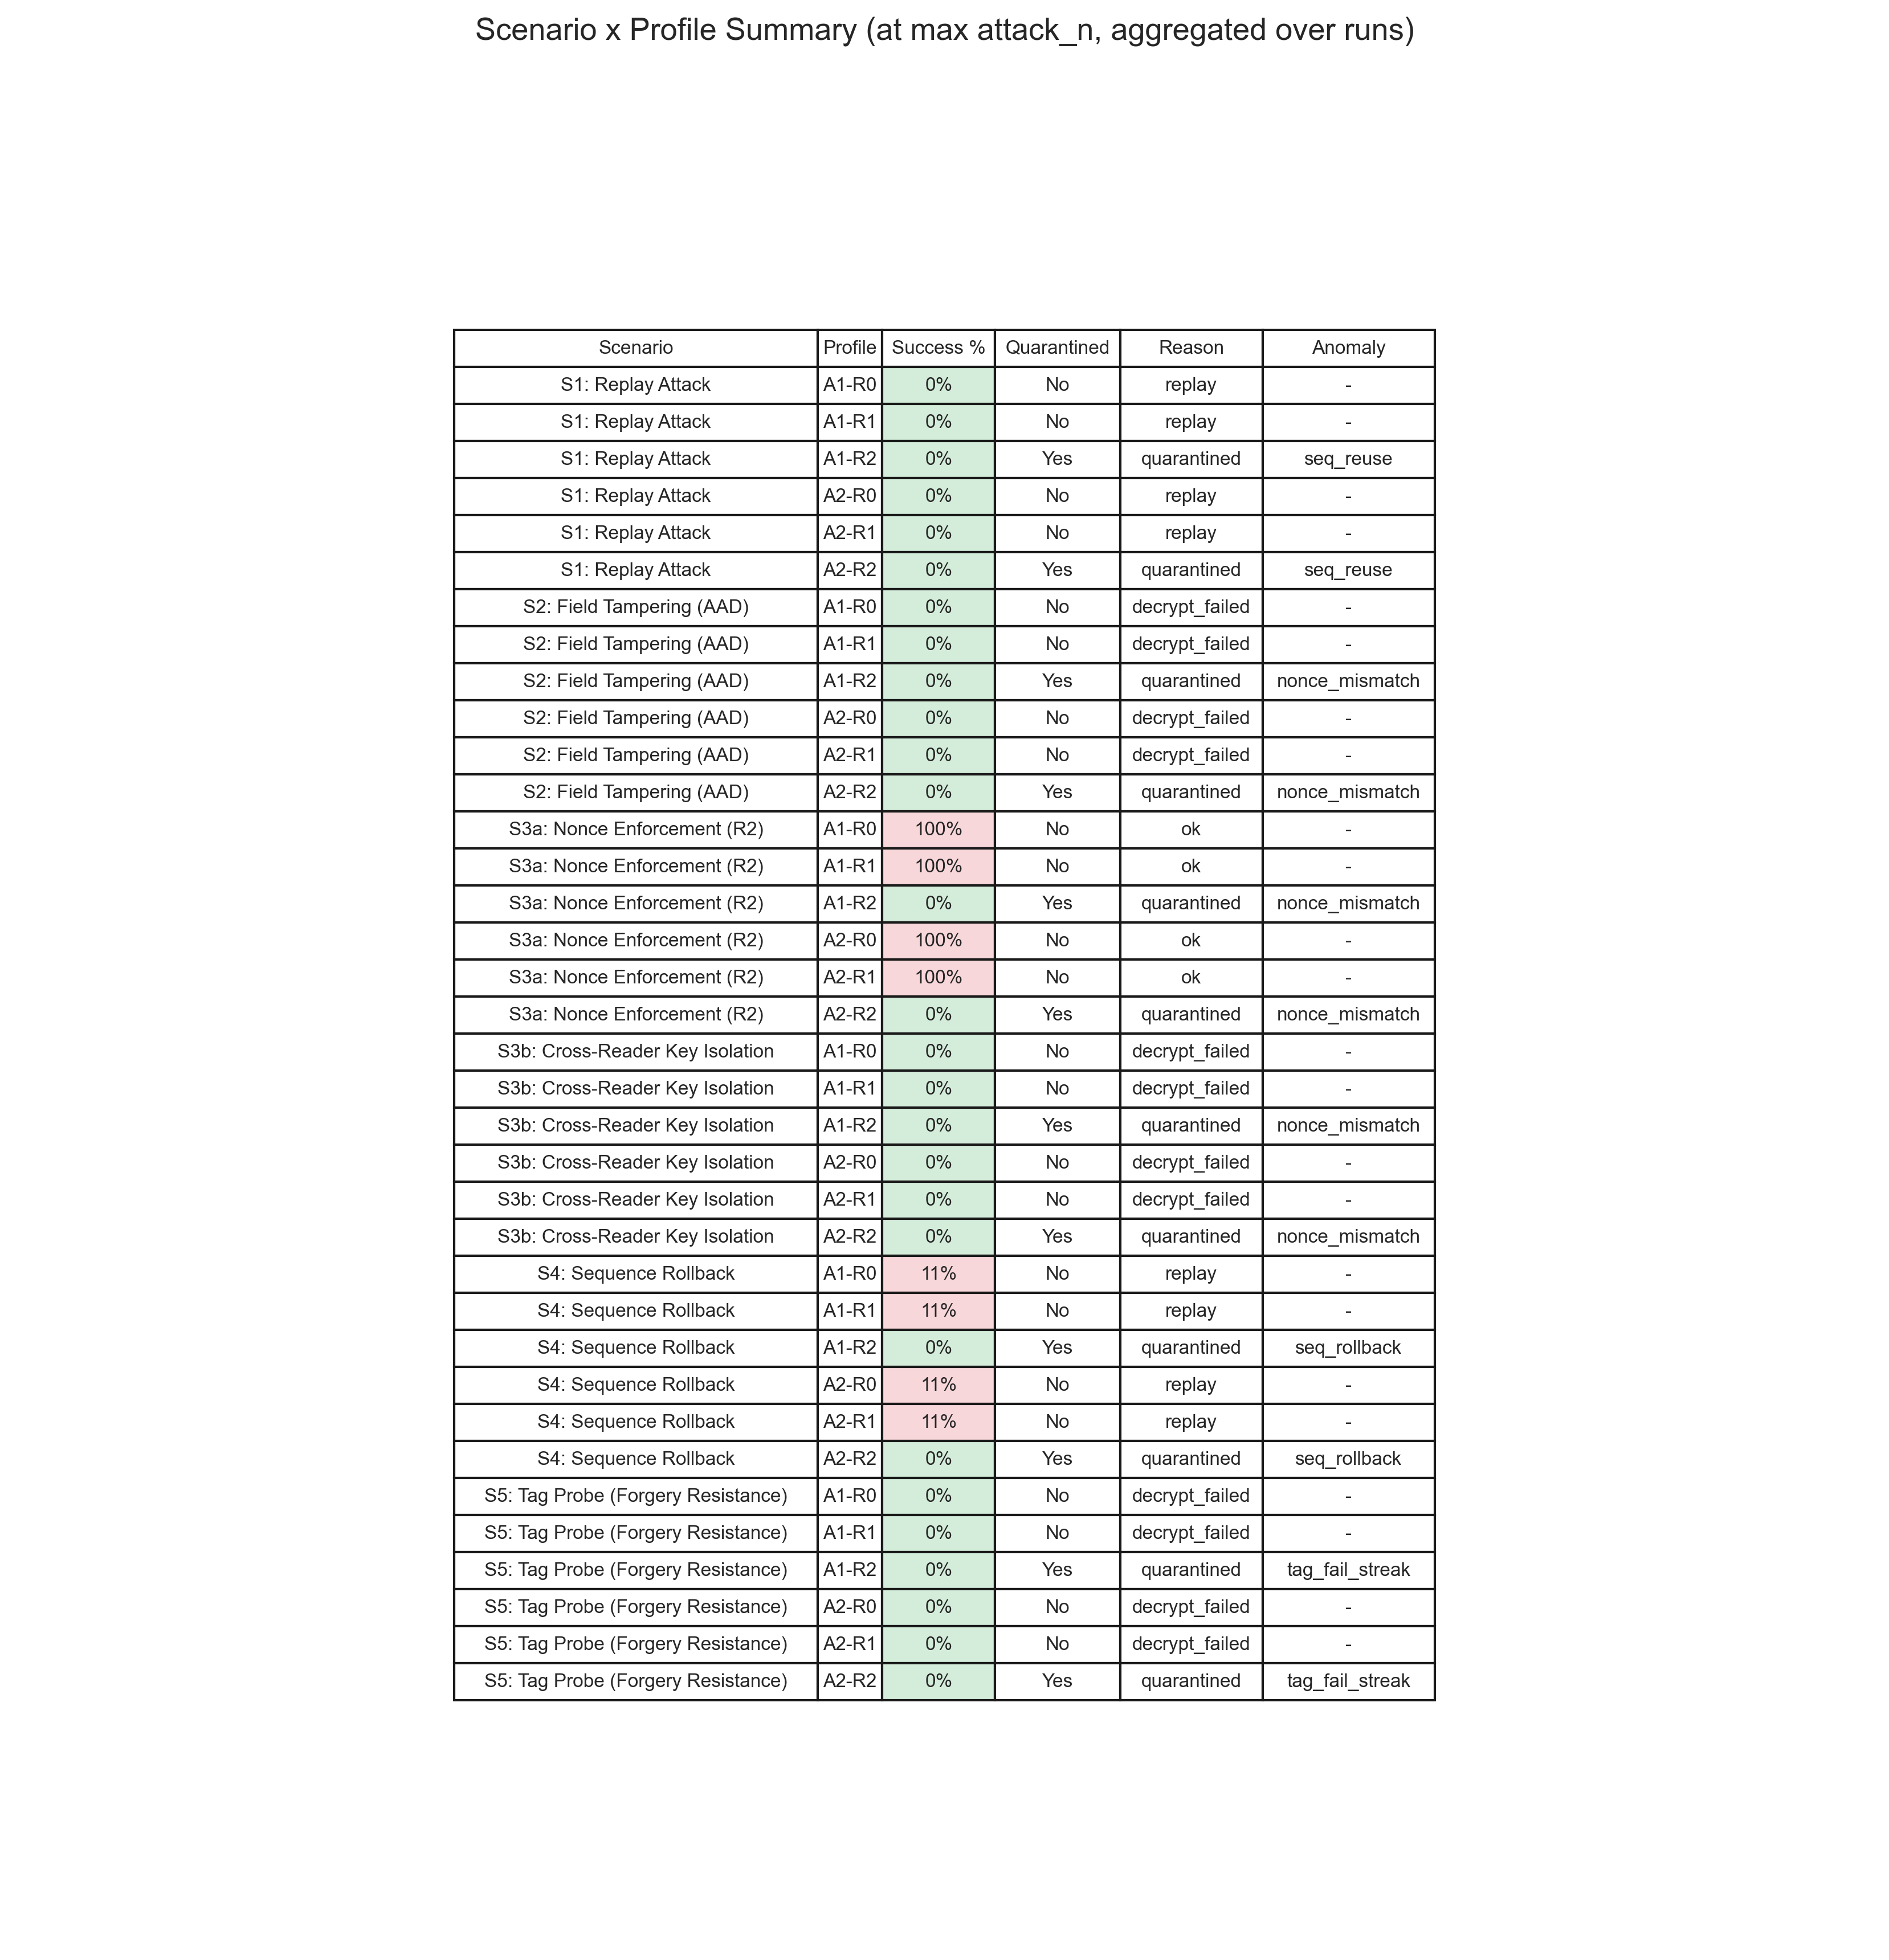
\includegraphics[width=\linewidth]{plots/scenario_summary_table.png}
\caption{Súhrnná tabuľka výsledkov experimentov: scenár $\times$ profil.}
\label{fig:summary_table}
\end{figure}

\noindent Obrázok~\ref{fig:summary_table} poskytuje prehľad výsledkov všetkých scenárov a profilov. Experimentálna analýza šiestich scenárov naprieč šiestimi konfiguračnými profilmi potvrdila nasledujúce zistenia:

\begin{enumerate}[leftmargin=*,itemsep=2pt]
  \item \textbf{Nulová false reject rate:} Žiadny validný frame nebol zamietnutý žiadnym profilom.
  \item \textbf{Nonce enforcement a HKDF izolácia (S3a/S3b):} S3a ukazuje, že R2 ako jediný vynucuje nonce politiku --- poistka pre budúce škálovanie. S3b potvrdzuje, že HKDF per-reader derivácia izoluje kľúčový materiál medzi čítačkami naprieč všetkými profilmi.
  \item \textbf{R2 zablokoval všetky testované scenáre:} 0\% úspešnosť naprieč S1--S5 v~rámci tejto experimentálnej sady (vrátane S3a, ktorý je komponentovou validáciou nonce mechanizmu, nie simuláciou externého útoku).
  \item \textbf{Replay window a detektor sú komplementárne:} S4 odhaľuje štruktúrnu medzeru replay window, ktorú detektor uzatvára.
  \item \textbf{AAD binding je fundamentálna ochrana:} Funguje nezávisle od nonce režimu.
  \item \textbf{Karanténa pridáva proaktívnu izoláciu zariadení:} Kvalitativne odlišná od per-frame odmietnutia.
  \item \textbf{Overhead detektora (${\sim}19\%$):} Pri reálnej záťaži prístupového systému ($<$10 udalostí/s) rádovo nepodstatný; pri vyššej záťaži by mal byť zohľadnený.
  \item \textbf{Výsledky sú reprodukovateľné:} Všetkých 5 behov (seedy 42--46) poskytlo zhodné výsledky attack success rate. Bezpečnostné mechanizmy sú invariantné voči hodnotám nonce --- 5 behov tu neplní úlohu štatistického vzorku, ale overenia konzistencie výsledkov.
\end{enumerate}

Tieto výsledky potvrdujú pôvodnú hypotézu práce: kombinácia AEAD s AAD binding, deterministickým nonce a runtime anomálnou detekciou (profil R2) \textbf{materiálne zvyšuje odolnosť} prístupového systému v porovnaní so základnými konfiguráciami, a to pri prijateľnom výkonnostnom overheade.


% ==============================================================
% ==============================================================
% Kapitola: Záver
% ==============================================================

\section{Záver}
\label{sec:conclusion}

Táto práca sa zaoberala návrhom, implementáciou a experimentálnym hodnotením bezpečnostných mechanizmov pre systém kontroly fyzického prístupu postavený na bezkontaktných identifikátoroch RFID/NFC. Výsledkom je funkčný prototyp a jeho systematická analýza, ktorá identifikuje konkrétne prínosy jednotlivých bezpečnostných vrstiev.

\subsection{Súhrn realizovaných prác}

V rámci práce boli realizované nasledujúce kroky:

\begin{enumerate}[leftmargin=*,itemsep=3pt]
  \item \textbf{Teoretická analýza.} Rozobrané boli bezpečnostné pojmy (CIA triáda, AAA model, RBAC), kryptografické primitíva (AEAD, HMAC, HKDF), návrh bezpečných protokolov (fail-closed, kanonizácia, anti-replay) a špecifiká RFID/NFC technológií vrátane známych útokov na MIFARE Classic\cite{GarciaMIFARE2008}. Analýza bola orientovaná na prax --- každý teoretický koncept je priamo naviazaný na konkrétny mechanizmus v prototype.

  \item \textbf{Návrh a implementácia prototypu.} Prototyp pozostáva z hardvérovej čítačky (ESP32 + RC522\cite{Espressif2024}), serverovej aplikácie v jazyku C++20 a lokálneho úložiska SQLite. Systém implementuje viacvrstvovú ochranu:
  \begin{itemize}[itemsep=1pt]
    \item HMAC-SHA-256 autentifikácia hardvérových požiadaviek,
    \item interný AEAD frame (ChaCha20-Poly1305\cite{RFC8439} / XChaCha20-Poly1305\cite{XChaChaDraft}) s AAD väzbou hlavičky,
    \item HKDF derivácia per-reader kľúčov\cite{RFC5869} s verziovaním a domain separation,
    \item tri stratégie generovania nonce (náhodný, deterministický HMAC, deterministický s runtime verifikáciou),
    \item \texttt{ProtocolAnomalyDetector} so schopnosťou karantény zariadení,
    \item sliding window anti-replay mechanizmus,
    \item tamper-evident auditný log s HMAC hash chain\cite{SchneierKelsey1999} a anchor ochranou,
    \item RBAC model s pepper-chránenými identifikátormi kariet.
  \end{itemize}
  Kódová báza je modulárna (9~modulov), písaná v štandarde C++20 s výhradným použitím knižnice libsodium pre kryptografické operácie\cite{LibsodiumXChaChaDoc}.

  \item \textbf{Verifikácia kvality kódu.} Pred experimentmi bola vykonaná statická analýza (\texttt{clang-tidy}\cite{ClangTidy}: 0~bezpečnostných nálezov) a dynamická analýza (ASan\cite{AddressSanitizer}, UBSan, LSan: 0~nálezov za behu). Testovacia sada\cite{GoogleTest} obsahuje 44~testovacích prípadov pokrývajúcich kryptografiu, replay window, auditný log a rozhodovaciu logiku.

  \item \textbf{Experimentálna analýza.} Navrhnutý a implementovaný bol C++ experimentálny harness, ktorý zdieľa produkčný kód a umožňuje reprodukovateľné testy. Šesť konfiguračných profilov (2~algoritmy $\times$ 3~nonce stratégie) bolo testovaných v šiestich scenároch (replay, AAD tampering, cross-reader key isolation, seq rollback, tag forgery resistance, throughput benchmark). Každý scenár bežal 5-krát, celkový objem dát presahuje 2{,}8~milióna meraní.

  \item \textbf{Analýza a vizualizácia výsledkov.} Python pipeline spracúva CSV výstupy do siedmich grafov a troch LaTeX tabuliek s~chybovými pásmami a~intervalmi spoľahlivosti.
\end{enumerate}

\subsection{Hlavné výsledky a závery}

Experimentálna analýza potvrdila šesť hlavných tézisov:

\begin{table}[htbp]
\renewcommand{\arraystretch}{1.3}
\centering
\caption{Súhrn hlavných experimentálnych zistení}
\label{tab:findings}
\small
\begin{tabular}{c p{10.5cm}}
\toprule
\textbf{Tézis} & \textbf{Zistenie} \\
\midrule
T1 & R2 ako jediný vynucuje nonce politiku (S3a: R0/R1 100\% úspešnosť vs.\ R2 0\%) --- bezpečnostná poistka pre budúce škálovanie. HKDF per-reader derivácia zabraňuje cross-reader útokom (S3b: 0\% úspešnosť naprieč všetkými profilmi). \\
T2 & \texttt{ProtocolAnomalyDetector} (profily R2) dosiahol 0\% úspešnosť naprieč všetkými testovanými scenármi (S1--S5). V S3a a S4 bol jediným mechanizmom, ktorý scenár úplne zastavil; v S3b a S5 pridáva operačnú eskaláciu (karanténu). \\
T3 & Replay window a anomálna detekcia sú komplementárne. S4 odhaľuje štruktúrnu medzeru replay window (56 z 500 frame prejde), ktorú detektor uzatvára cez rollback detekciu. \\
T4 & AAD binding poskytuje ochranu nezávisle od režimu nonce --- S2 ukazuje 0\% úspešnosť manipulácie hlavičky naprieč všetkými profilmi. \\
T5 & Karanténa zariadení mení reakciu systému z reaktívnej (odmietnutie frame) na proaktívnu (izolácia zariadenia) --- realizácia defense-in-depth\cite{DefenseInDepth}. \\
T6 & Overhead detektora (${\sim}19\%$ pokles priepustnosti, ${\sim}35\,\mu$s na frame) je rádovo nepodstatný pre reálnu prevádzku prístupového systému ($<$10 udalostí/s), hoci nie je zanedbateľný. \\
\bottomrule
\end{tabular}
\end{table}

\noindent Kľúčovým zistením je, že profil R2 (deterministický nonce s aktívnym detektorom) v kombinácii s~existujúcimi vrstvami (AEAD + AAD + HKDF + anti-replay + audit) poskytuje \textbf{materiálne vyššiu odolnosť} voči všetkým testovaným triedam útokov pri prijateľnom výkonnostnom overheade. Zároveň experiment potvrdzuje, že \textbf{voľba algoritmu} (A1 vs.\ A2) nemá merateľný vplyv na bezpečnostné metriky --- oba algoritmy sú ekvivalentné v odolnosti a porovnateľné vo výkone.

Všetkých 5 behov (seedy 42--46) poskytlo zhodné výsledky bezpečnostných metrík, čo naznačuje, že pozorované rozdiely vychádzajú z architektonických vlastností systému, nie z konkrétnych hodnôt nonce.

\subsection{Splnenie cieľov práce}

\begin{table}[htbp]
\renewcommand{\arraystretch}{1.3}
\centering
\caption{Mapovanie cieľov práce na realizované výstupy}
\label{tab:goals-mapping}
\begin{tabular}{c p{5.8cm} p{5.8cm}}
\toprule
\textbf{Cieľ} & \textbf{Definícia} & \textbf{Realizácia} \\
\midrule
C1 & Analýza bezpečnostných hrozieb & Kapitoly 3--8: CIA triáda, STRIDE\cite{STRIDE}, RFID/NFC hrozby, kryptografické základy \\
C2 & Návrh bezpečnostného protokolu & Kapitoly 9--10: HMAC autentifikácia, AEAD frame, anti-replay, audit \\
C3 & Implementácia prototypu & Kapitola 21: 9 C++ modulov, ESP32 firmware, SQLite úložisko \\
C4 & Verifikácia kvality kódu & Kapitola 22: clang-tidy, sanitizers, 44 testov \\
C5 & Experimentálne hodnotenie & Kapitola 23: 6 profilov $\times$ 6 scenárov $\times$ 5 behov \\
\bottomrule
\end{tabular}
\end{table}

\subsection{Otvorené otázky a obmedzenia}

Napriek pozitívnym výsledkom je potrebné identifikovať obmedzenia, ktoré ovplyvňujú interpretáciu a prenášateľnosť záverov:

\begin{enumerate}[leftmargin=*,itemsep=3pt]
  \item \textbf{UID nie je kryptografický dôkaz identity.} Karty typu MIFARE Classic\cite{GarciaMIFARE2008} alebo iné karty bez vzájomnej autentifikácie umožňujú emuláciu UID. Prototyp sa spolieha na to, že bezpečnosť je zabezpečená na úrovni protokolu (HMAC + AEAD), nie na úrovni karty. Nasadenie kryptograficky silných kariet (napr. MIFARE DESFire) by eliminovalo túto závislosť.

  \item \textbf{Absencia TLS.} Komunikácia medzi čítačkou a serverom nie je šifrovaná na transportnej vrstve. V lokálnej sieti je HMAC autentifikácia dostatočná na zabránenie podvrhnutiu, no v sieťach s nedôveryhodnou infraštruktúrou by bolo nutné doplniť TLS\cite{RFC8446} alebo mTLS.

  \item \textbf{Jednostranná autentifikácia.} Server autentifikuje čítačku (cez HMAC), ale čítačka neautentifikuje server. Man-in-the-middle útočník by teoreticky mohol zachytávať odpovede. Pre produkčné nasadenie by bolo vhodné zvážiť vzájomnú autentifikáciu\cite{RFC9325}.

  \item \textbf{Lokálna SQLite databáza.} V aktuálnom riešení je databáza uložená na rovnakom stroji ako server. Útočník s fyzickým prístupom k serveru môže modifikovať databázu aj audit anchor. Produkčné nasadenie by vyžadovalo vzdialený anchor alebo HSM\cite{NIST80057}.

  \item \textbf{Rozsah testovaných scenárov.} Šesť scenárov pokrýva hlavné triedy útokov, no nepokrýva napríklad timing útoky, side-channel analýzu, alebo útoky na firmware čítačky. Rozšírenie sady scenárov by zvýšilo dôveru v kompletnosť hodnotenia.

  \item \textbf{Jednoprocesový server.} Aktuálna implementácia beží ako jeden proces s jedným vláknom pre spracovanie požiadaviek. Škálovanie na viacero čítačiek v reálnom nasadení by vyžadovalo asynchronné spracovanie alebo viacprocesový model.
\end{enumerate}

\subsection{Možnosti rozšírenia}

Na základe identifikovaných obmedzení a skúseností z implementácie je možné navrhnúť niekoľko smerov budúceho vývoja:

\begin{description}[leftmargin=*,itemsep=3pt]
  \item[Integrácia TLS/mTLS:] Doplnenie šifrovanej transportnej vrstvy s certifikátovou autentifikáciou zariadení\cite{RFC8446,RFC9325}. ESP32 podporuje TLS cez mbedTLS, čo umožňuje implementáciu bez zmeny hardvéru.

  \item[Podpora kryptografických kariet:] Prechod z jednoduchého čítania UID na vzájomnú autentifikáciu s kartou (napr. MIFARE DESFire EV3). Tým by sa eliminovala závislosť na serverovej kompenzácii slabej identity karty.

  \item[Fuzz testing:] Systematické testovanie vstupných parserov a kryptografických rozhraní pomocou AFL++ alebo libFuzzer s~cieľom nájsť edge cases, ktoré jednotkové testy nepokrývajú.

  \item[Distribuovaná architektúra:] Rozšírenie na viacero serverov s centralizovanou správou kľúčov a federovaným auditom. Anchor by bol uložený na nezávislom serveri alebo v~blockchain-like štruktúre.

  \item[Rotácia pepperu s online migráciou:] Implementácia bezprestojovej migrácie pepper verzie, kde sa existujúce karty postupne re-hashujú pri prvom použití pod novou verziou.

  \item[Adaptívna karanténa:] Rozšírenie \texttt{ProtocolAnomalyDetector} o časovo obmedzenú karanténu s~eskaláciou (napr. 1. incident: 5~minút; 2. incident: 1~hodina; 3. incident: trvalá karanténa). Aktuálna implementácia používa trvalú karanténu, čo je bezpečné, ale menej flexibilné.

  \item[Offline režim čítačky:] Podpora scenárov, kde čítačka dočasne stratí spojenie so serverom. Toto vyžaduje lokálnu cache posledných autorizácií a následnú synchronizáciu, čo prináša nové bezpečnostné výzvy (stale cache, conflict resolution).

  \item[Monitoring a alerting:] Integrácia s existujúcimi monitorovacími systémami (Prometheus, Grafana) pre vizualizáciu prevádzkových metrík a automatické upozornenia pri detekcii anomálií\cite{NIST80094}.
\end{description}

\subsection{Záverečné zhodnotenie}

Práca demonštruje, že aj v prototypovom prostredí je možné implementovať viacvrstvový bezpečnostný systém, ktorý poskytuje merateľnú ochranu voči realistickým útokovým scenárom. Kľúčovým prínosom nie je samotná implementácia jednotlivých mechanizmov --- tie sú v literatúre dobre popísané --- ale ich \emph{systematická integrácia} a \emph{experimentálne overenie} interakcií medzi nimi.

Výsledky jasne ukazujú, že bezpečnosť nie je binárna vlastnosť (\uv{zabezpečené vs.\ nezabezpečené}), ale spektrum závislé od konkrétnej kombinácie mechanizmov. Profil R2 s~aktívnym anomálnym detektorom nie je \uv{lepší} v~abstraktnom zmysle --- je lepší v~presne definovaných scenároch (S3, S4), kde iné mechanizmy zlyhávajú. Iné mechanizmy (replay window, AAD binding, AEAD) sú zasa dostatočné v~scenároch, kde detektor nie je potrebný (S1, S2, S5).

Tento diferencovaný pohľad --- nie \uv{zapni všetko}, ale \uv{pochop, čo chráni proti čomu} --- je hlavným záverom experimentálnej časti a podľa záverov analýzy aj najdôležitejším prínosom tejto práce pre prax návrhu bezpečných systémov kontroly prístupu.


\bibliographystyle{IEEEtran}
\bibliography{bibliography}

\end{document}
